\documentclass[a4paper,12pt,openany]{report}

\usepackage{geometry}
\geometry{margin=2cm}
\usepackage[utf8]{inputenc}
\usepackage{polski}
\usepackage{graphicx}
\usepackage{enumitem}
\usepackage{amsmath}
\usepackage{index}
\usepackage{subcaption}
\usepackage{hyperref}
\hypersetup{
    colorlinks=true,
    linkcolor=blue,
    filecolor=magenta,      
    urlcolor=cyan,
    pdftitle={Overleaf Example},
    pdfpagemode=FullScreen,
    }

\begin{document}

%%%%%%%%%%%%%%%%%%%%%%%%%%%%%%%%%%%%%%%%%%%%%%%%%%%%%%%%%%%%%%%%%%%%%%%%%%%%%%%%%%%%%%%%%%%%%%%%%%%%%%%%%%%%%%%%%%%%
%%%%%%%%%%%%%%%%%%%%%%%%%%%%%%%%%%%%%%%%%%%%%%%%%%%%%%%%%%%%%%%%%%%%%%%%%%%%%%%%%%%%%%%%%%%%%%%%%%%%%%%%%%%%%%%%%%%%
\title{\Large{\textbf{Wariacje filtrów uśredniających i wyostrzających w analizie obrazów.}}}
\author{Filip Matejko 249965}
\date{13.01.2022}
\maketitle

\tableofcontents

%%%%%%%%%%%%%%%%%%%%%%%%%%%%%%%%%%%%%%%%%%%%%%%%%%%%%%%%%%%%%%%%%%%%%%%%%%%%%%%%%%%%%%%%%%%%%%%%%%%%%%%%%%%%%%%%%%%%
%%%%%%%%%%%%%%%%%%%%%%%%%%%%%%%%%%%%%%%%%%%%%%%%%%%%%%%%%%%%%%%%%%%%%%%%%%%%%%%%%%%%%%%%%%%%%%%%%%%%%%%%%%%%%%%%%%%%
\chapter{Wstęp}

\paragraph{\indent Coraz częściej do analizy obrazów wykorzystuje się komputery. Jednym ze sposobów poprawy skuteczności pracy systemów do analizy obrazów jest stosowanie filtrów. Filtry dobiera się w odpowiednio w zależności od tego co chce się osiągnąć.}

\paragraph{\indent W tej pracy opisuję działanie 2 wybranych filtrów - uśredniający (wygładzający) i wyostrzający. Analizie poddam również wpływ wielkości i kształtu filtrów na efekt końcowy.}

\paragraph{\indent W celu pokazania działania filtrów wykorzystuję je w splocie ze zdjęciem Lenny. Zdjęcie te jest wykorzystywane do testowania algorytmów do analizy obrazów ze względu na dużą ilość elementów sprawiających trudności - gładkie przejścia, ostre krawędzie itp \href{https://en.wikipedia.org/wiki/Lenna}{[1]}. W celu ułatwienia wykonania splotu i analizy filtrów wykorzystuję zdjęcie w wersji czarno białej. W takiej sytuacji filtr ma postać macierzy dwuwymiarowej. W splocie zdjęcia kolorowego należałoby wykorzystać macierz trójwymiarową (ze względu na 3 kanały - RGB).}

\begin{center}
\includegraphics[width=10cm]{resources/Lena.jpg}\\
\tiny{Lenna}
\end{center}

\chapter{Filtry}

\section{Filtr uśredniający}
\text{Przykład filtru uśredniającego:}
\\
\linebreak
$\begin{pmatrix}
0.25 & 0.25\\
0.25 & 0.25
\end{pmatrix}$
\\
\linebreak
\text{Wyznaczanie wartości w macierzy:}
\\
\linebreak
\begin{gather*}
W - \text{liczba wierszy} \\
K - \text{liczba kolumn} \\
n[w, k] - \text{wartość macierzy w wierszu 'w' i kolumnie 'k'} \\
n[w, k] = \frac{1}{w*k}\\
\end{gather*}
\\
\linebreak
\text{Wykorzystane rozmiary macierzy:}
\begin{itemize}
\item 3x3
\item 5x5
\item 10x10
\item 20x20
\item 40x40
\item 20x5
\item 5x20
\item 40x5
\item 5x40
\item 20x3
\item 3x20
\item 40x3
\item 3x40
\end{itemize}
\pagebreak

\section{Filtr wyostrzający}
\text{Przykład filtru uśredniającego:}
\\
\linebreak
$\begin{pmatrix}
0 & -1 & 0 \\
-1 & 5 & -1 \\
0 & -1 & 0 \\
\end{pmatrix}$
\\
\linebreak
\text{liczba wierszy i kolumn macierzy musi być nieparzysta.}
\\
\linebreak
\text{Wyznaczanie wartości w macierzy:}
\\
\linebreak
\begin{gather*}
W - \text{nieparzysta liczba wierszy} \\
K - \text{nieparzysta liczba kolumn} \\
n[w, k] - \text{wartość macierzy w wierszu 'w' i kolumnie 'k'} \\
\\
\text{jeśli w = W//2 oraz k = K//2 to:}\\
n[w, k] = W + K - 1\\
\\
\text{jeśli w = W//2 albo k = K//2 to:}\\
n[w, k] = -1\\
\\
text{pozostałe przypadki to:}\\
n[w, k] = 0\\
\end{gather*}
\\
\linebreak
\text{Wykorzystane rozmiary macierzy:}
\begin{itemize}
\item 3x3
\item 5x5
\item 7x7
\item 9x9
\item 11x11
\item 21x21
\item 9x5
\item 11x5
\item 21x5
\item 5x9
\item 5x11
\item 5x21
\item 9x3
\item 11x3
\item 21x3
\item 3x9
\item 3x11
\item 3x21
\end{itemize}
\pagebreak

%%%%%%%%%%%%%%%%%%%%%%%%%%%%%%%%%%%%%%%%%%%%%%%%%%%%%%%%%%%%%%%%%%%%%%%%%%%%%%%%%%%%%%%%%%%%%%%%%%%%%%%%%%%%%%%%%%%%
%%%%%%%%%%%%%%%%%%%%%%%%%%%%%%%%%%%%%%%%%%%%%%%%%%%%%%%%%%%%%%%%%%%%%%%%%%%%%%%%%%%%%%%%%%%%%%%%%%%%%%%%%%%%%%%%%%%%
\chapter{Działanie filtrów}

\paragraph{\indent Działanie filtru uśredniającego oraz wyostrzającego są analogiczne. Okno wielkości filtra przesuwa się po obrazie, jego zawartość jest wymnażana przez macierz filtra, a następnie sumowana. Przykład splotu z filtrem uśredniającym:}

\begin{center}
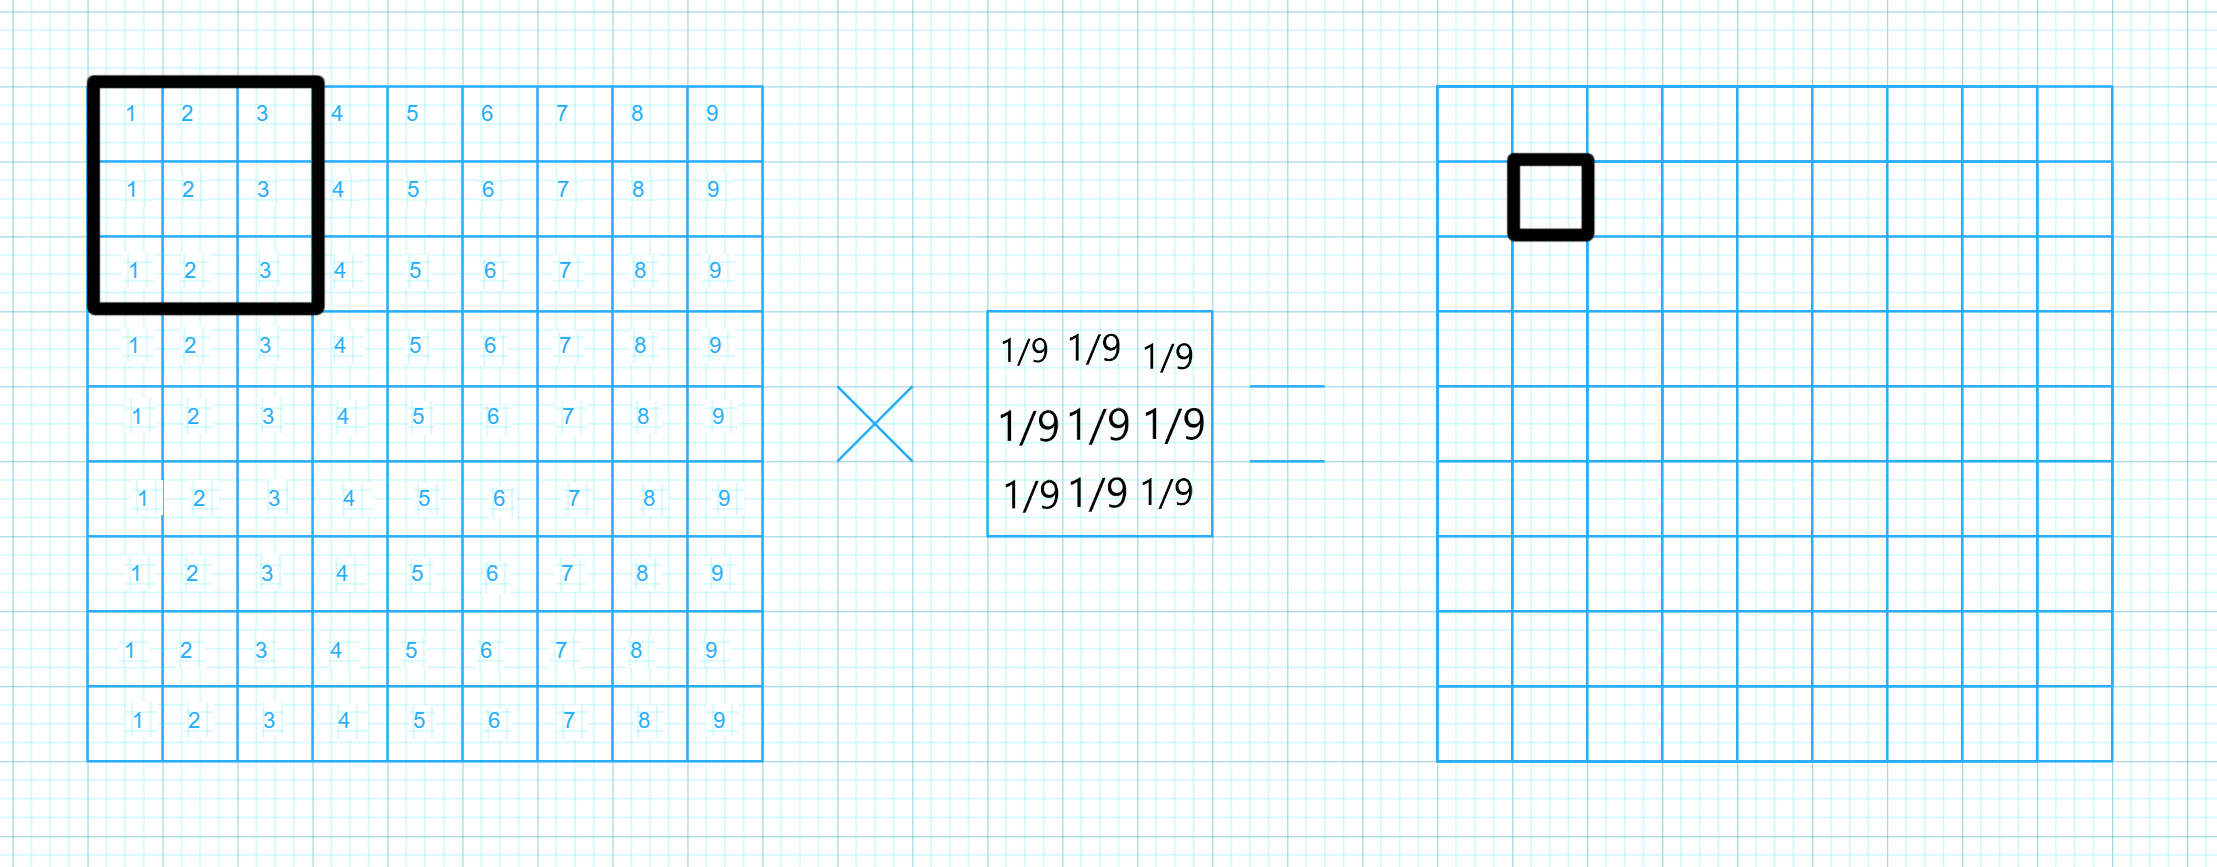
\includegraphics[width=13cm]{resources/blur1.png}
\linebreak
\tiny{Krok 1.}
\end{center}

\begin{center}
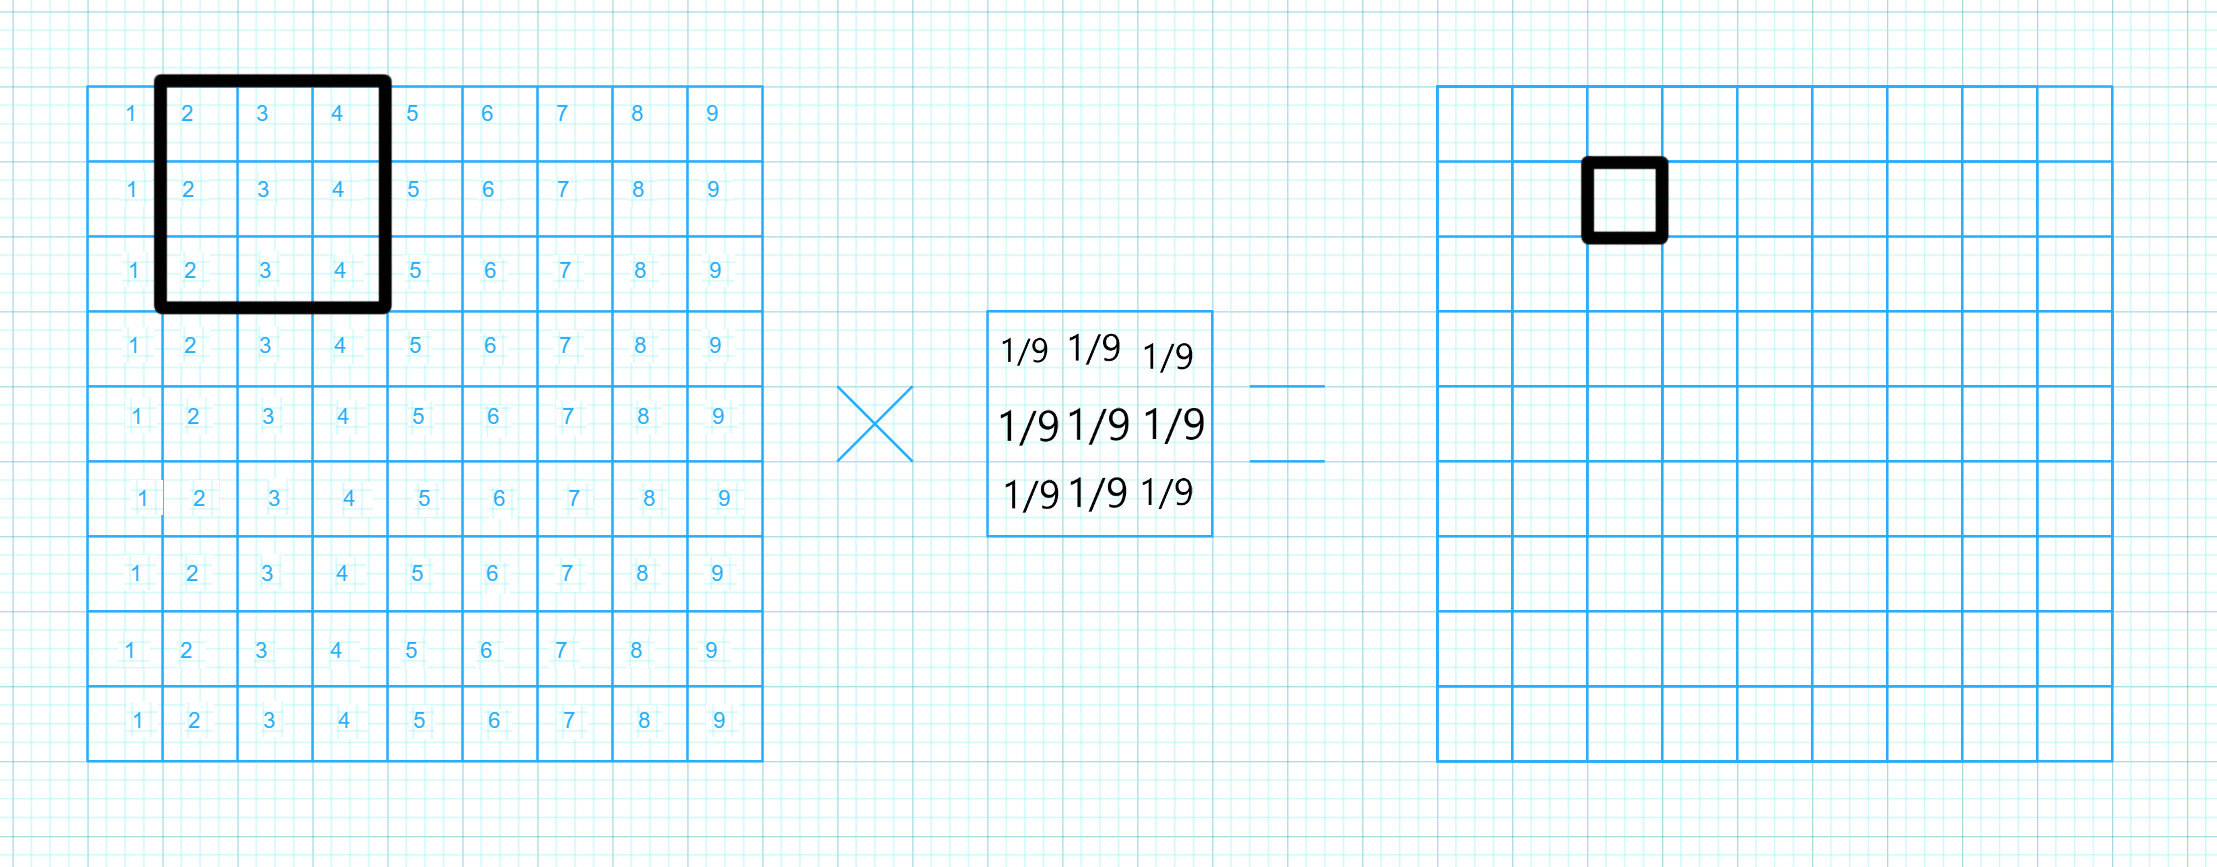
\includegraphics[width=13cm]{resources/blur2.png}
\linebreak
\tiny{Krok 2.}
\end{center}

\begin{center}
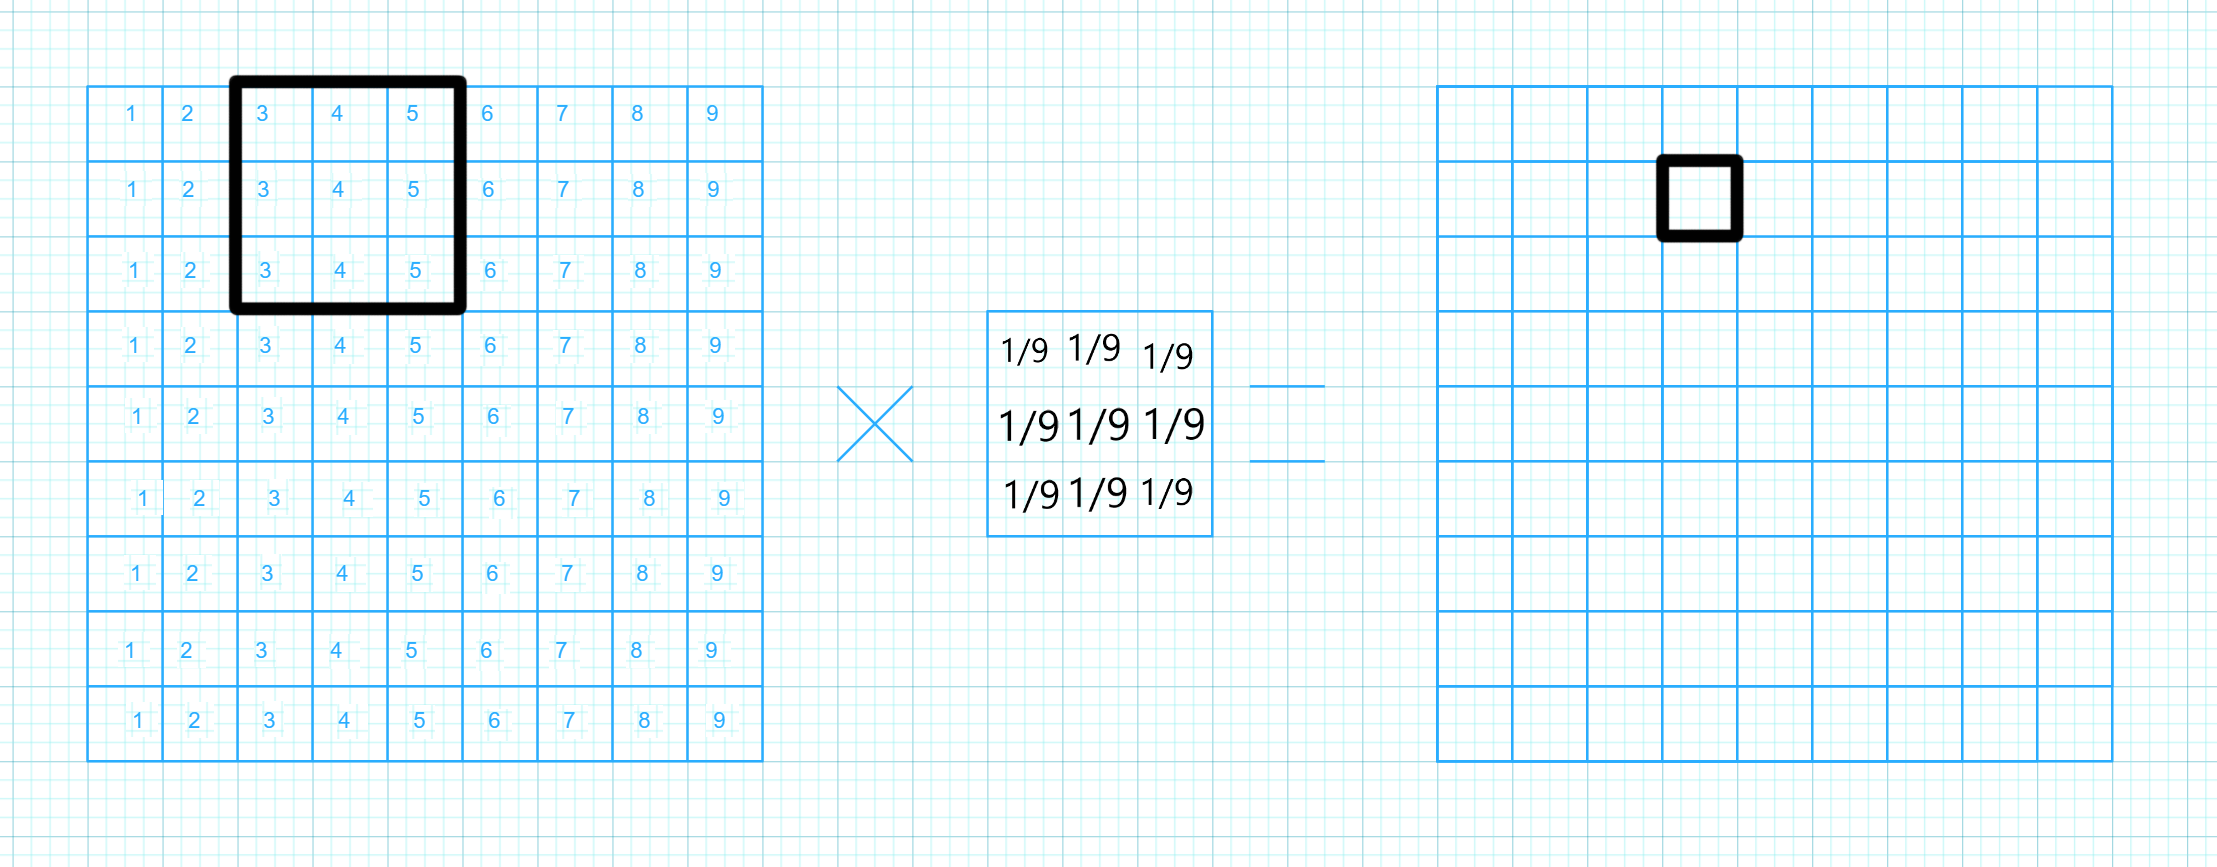
\includegraphics[width=13cm]{resources/blur3.png}
\linebreak
\tiny{Krok 3.}
\end{center}


\pagebreak
\paragraph{\indent Wartości na brzegach są otrzymywane przez rozszerzenie obrazu. Sposób wykorzystany w moim rozwiązaniu polega na odbiciu wartości przy krawędzi obrazu. Przykład odbicia względem prawej krawędzi obrazu:}

\begin{center}
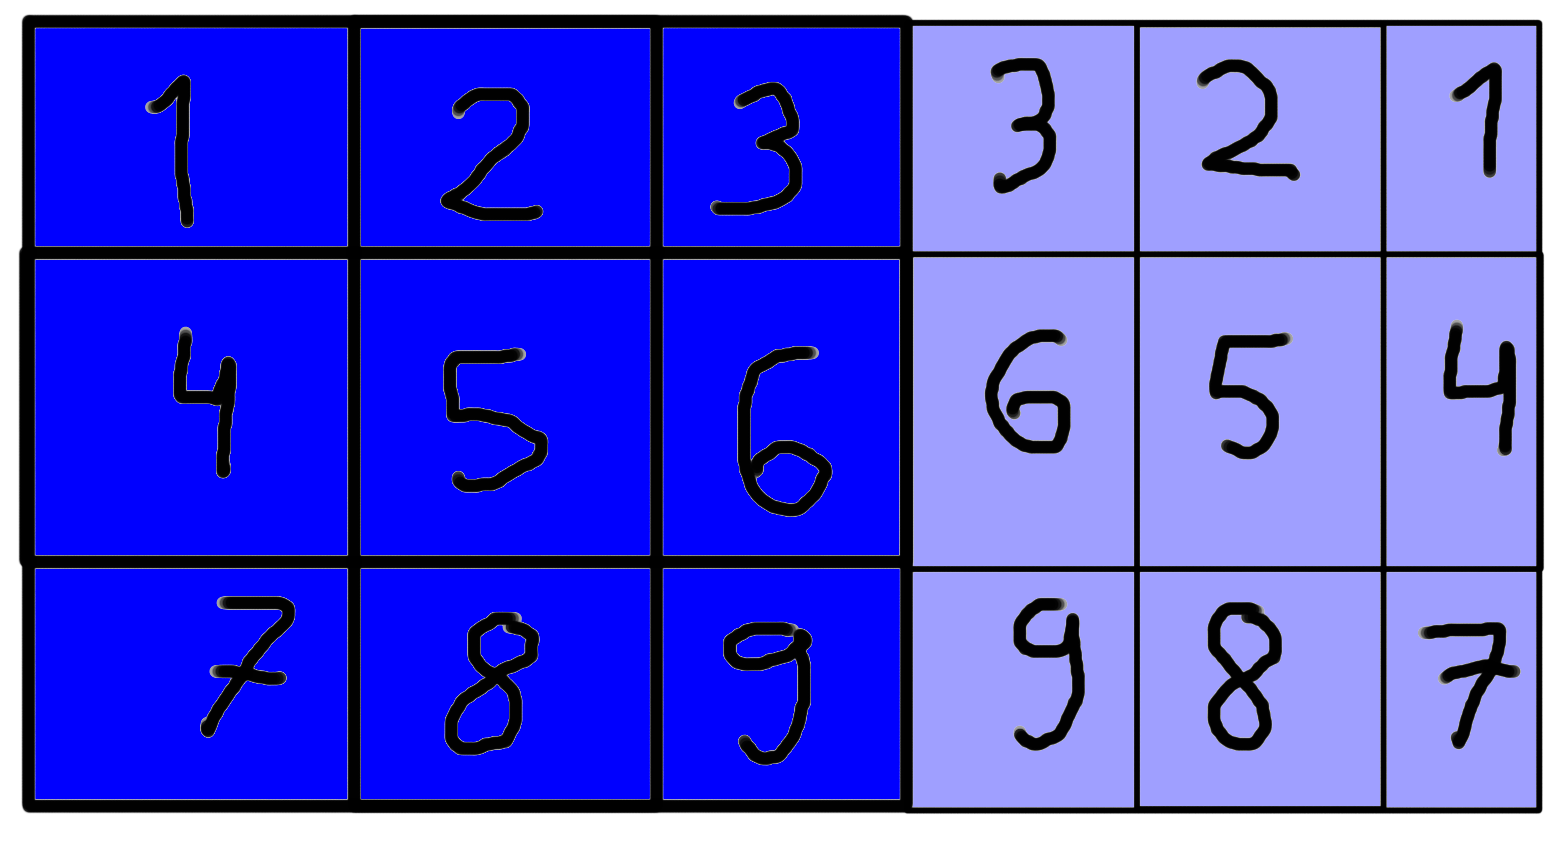
\includegraphics[width=10cm]{resources/reflect.png}
\linebreak
\tiny{Niebieskie pola wskazują obraz, fioletowe - odbicie.}
\end{center}

%%%%%%%%%%%%%%%%%%%%%%%%%%%%%%%%%%%%%%%%%%%%%%%%%%%%%%%%%%%%%%%%%%%%%%%%%%%%%%%%%%%%%%%%%%%%%%%%%%%%%%%%%%%%%%%%%%%%
%%%%%%%%%%%%%%%%%%%%%%%%%%%%%%%%%%%%%%%%%%%%%%%%%%%%%%%%%%%%%%%%%%%%%%%%%%%%%%%%%%%%%%%%%%%%%%%%%%%%%%%%%%%%%%%%%%%%
\chapter{Przykładowe wyniki filtracji}

\begin{center}
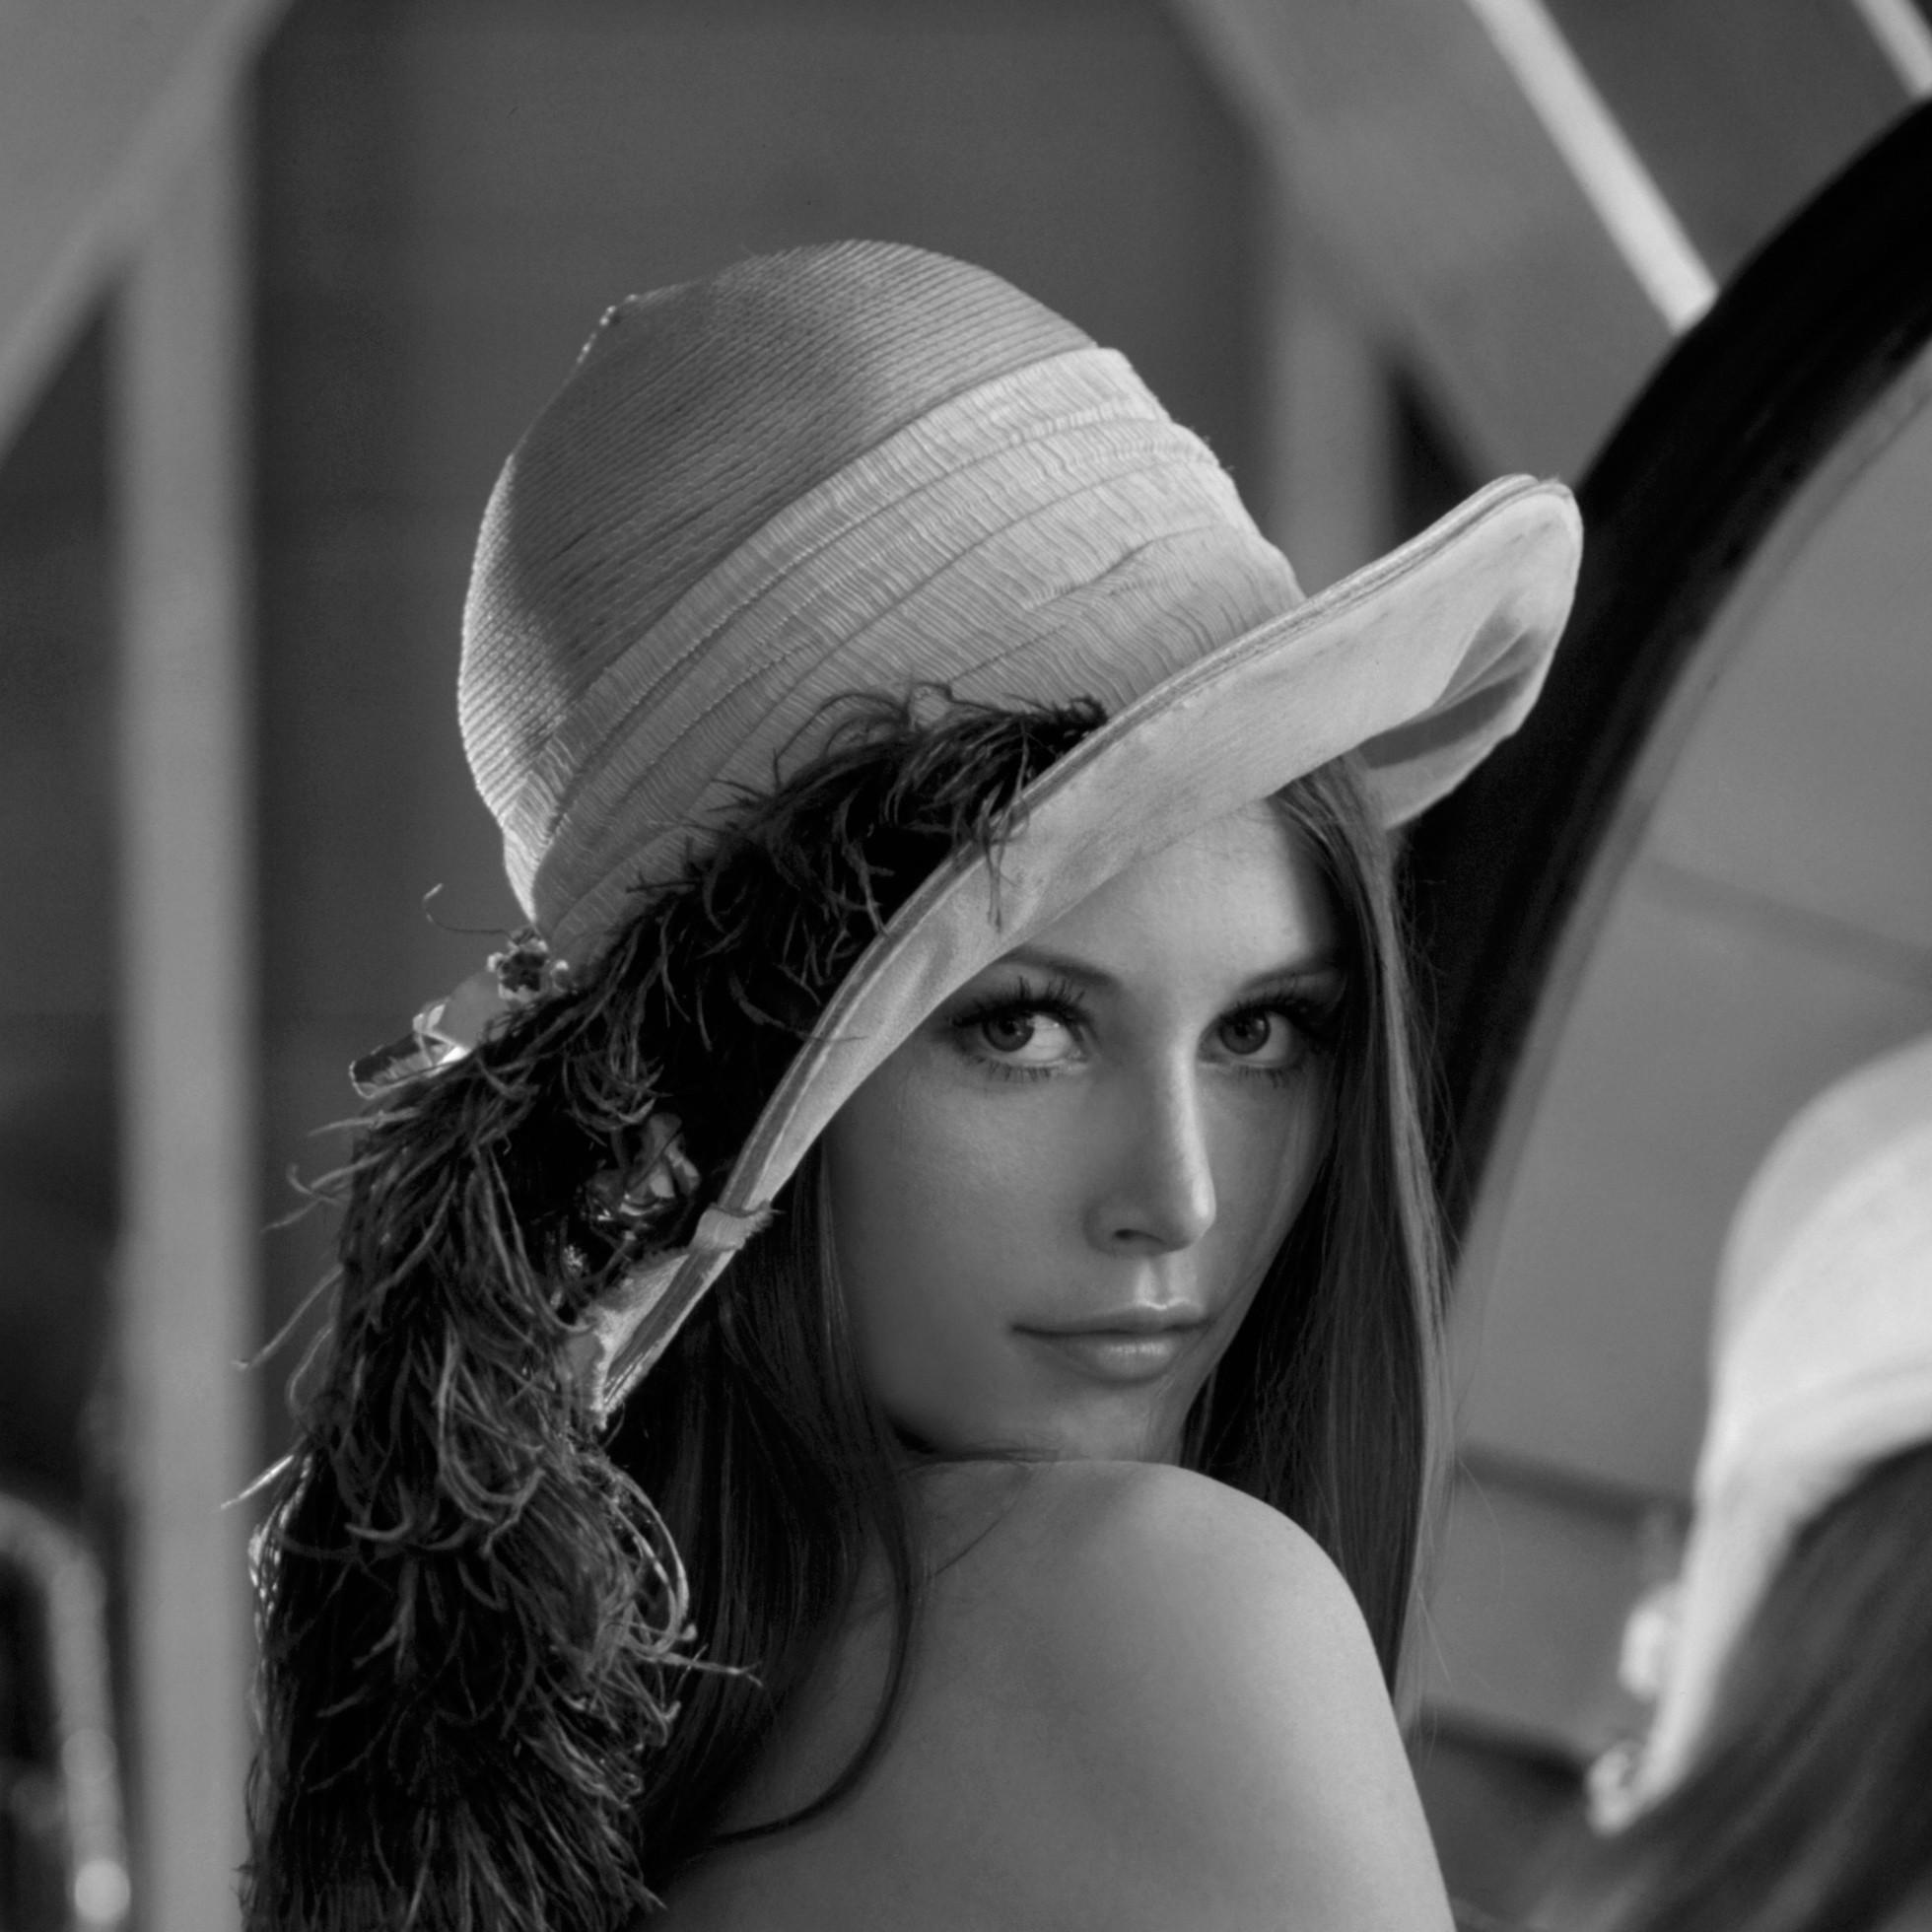
\includegraphics[width=15cm]{resources/modified/lena_gray.jpg}
\linebreak
\tiny{Czarno biała wersja zdjęcia źródłowego poddawana filtracji.}
\end{center}

%%%%%%%%%%%%%%%%%%%%%%%%%%%%%%%%%%%%%%%%%%%%%%%%%%%%%%%%%%%%%%%%%%%%%%%%%%%%%%%%%%%%%%%%%%%%%%%%%%%%%%%%%%%%%%%%%%%%%
\pagebreak
\section{Filtr uśredniający}

\begin{center}
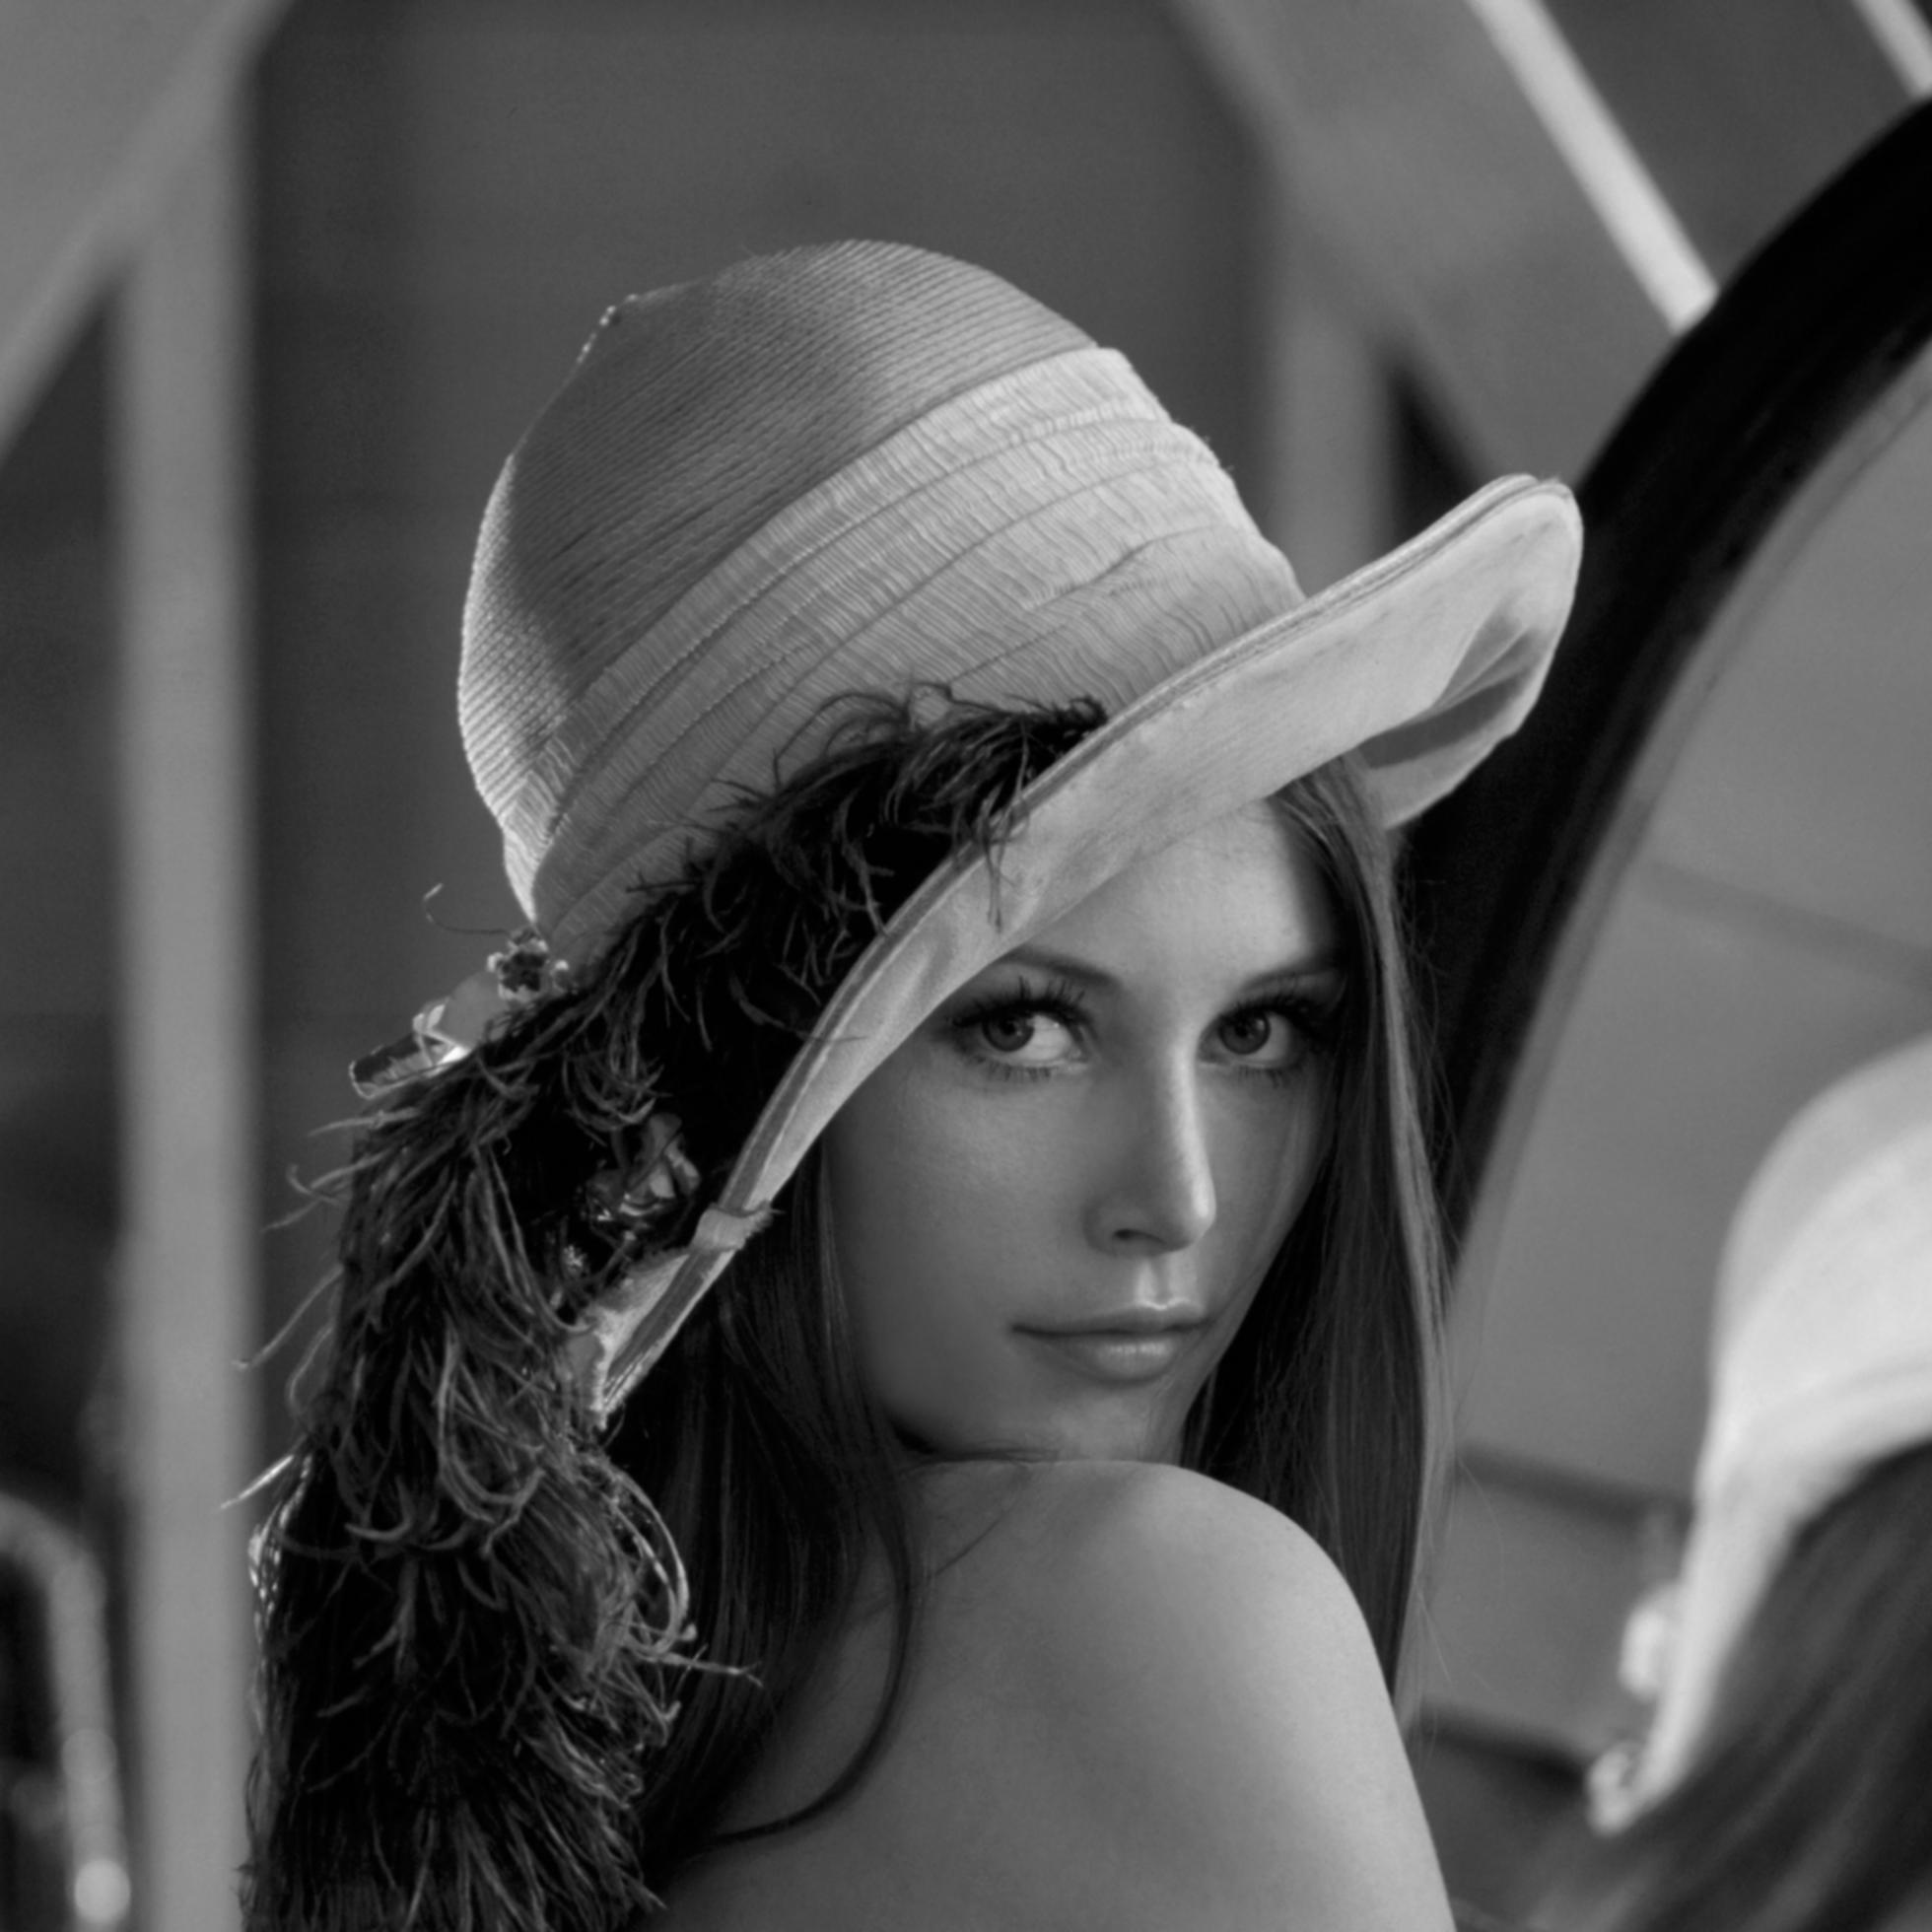
\includegraphics[width=7cm]{resources/modified/lena/lena_blur_3x3.jpg}
\linebreak
\tiny{Wynik działania filtru 3x3}
\end{center}

\begin{center}
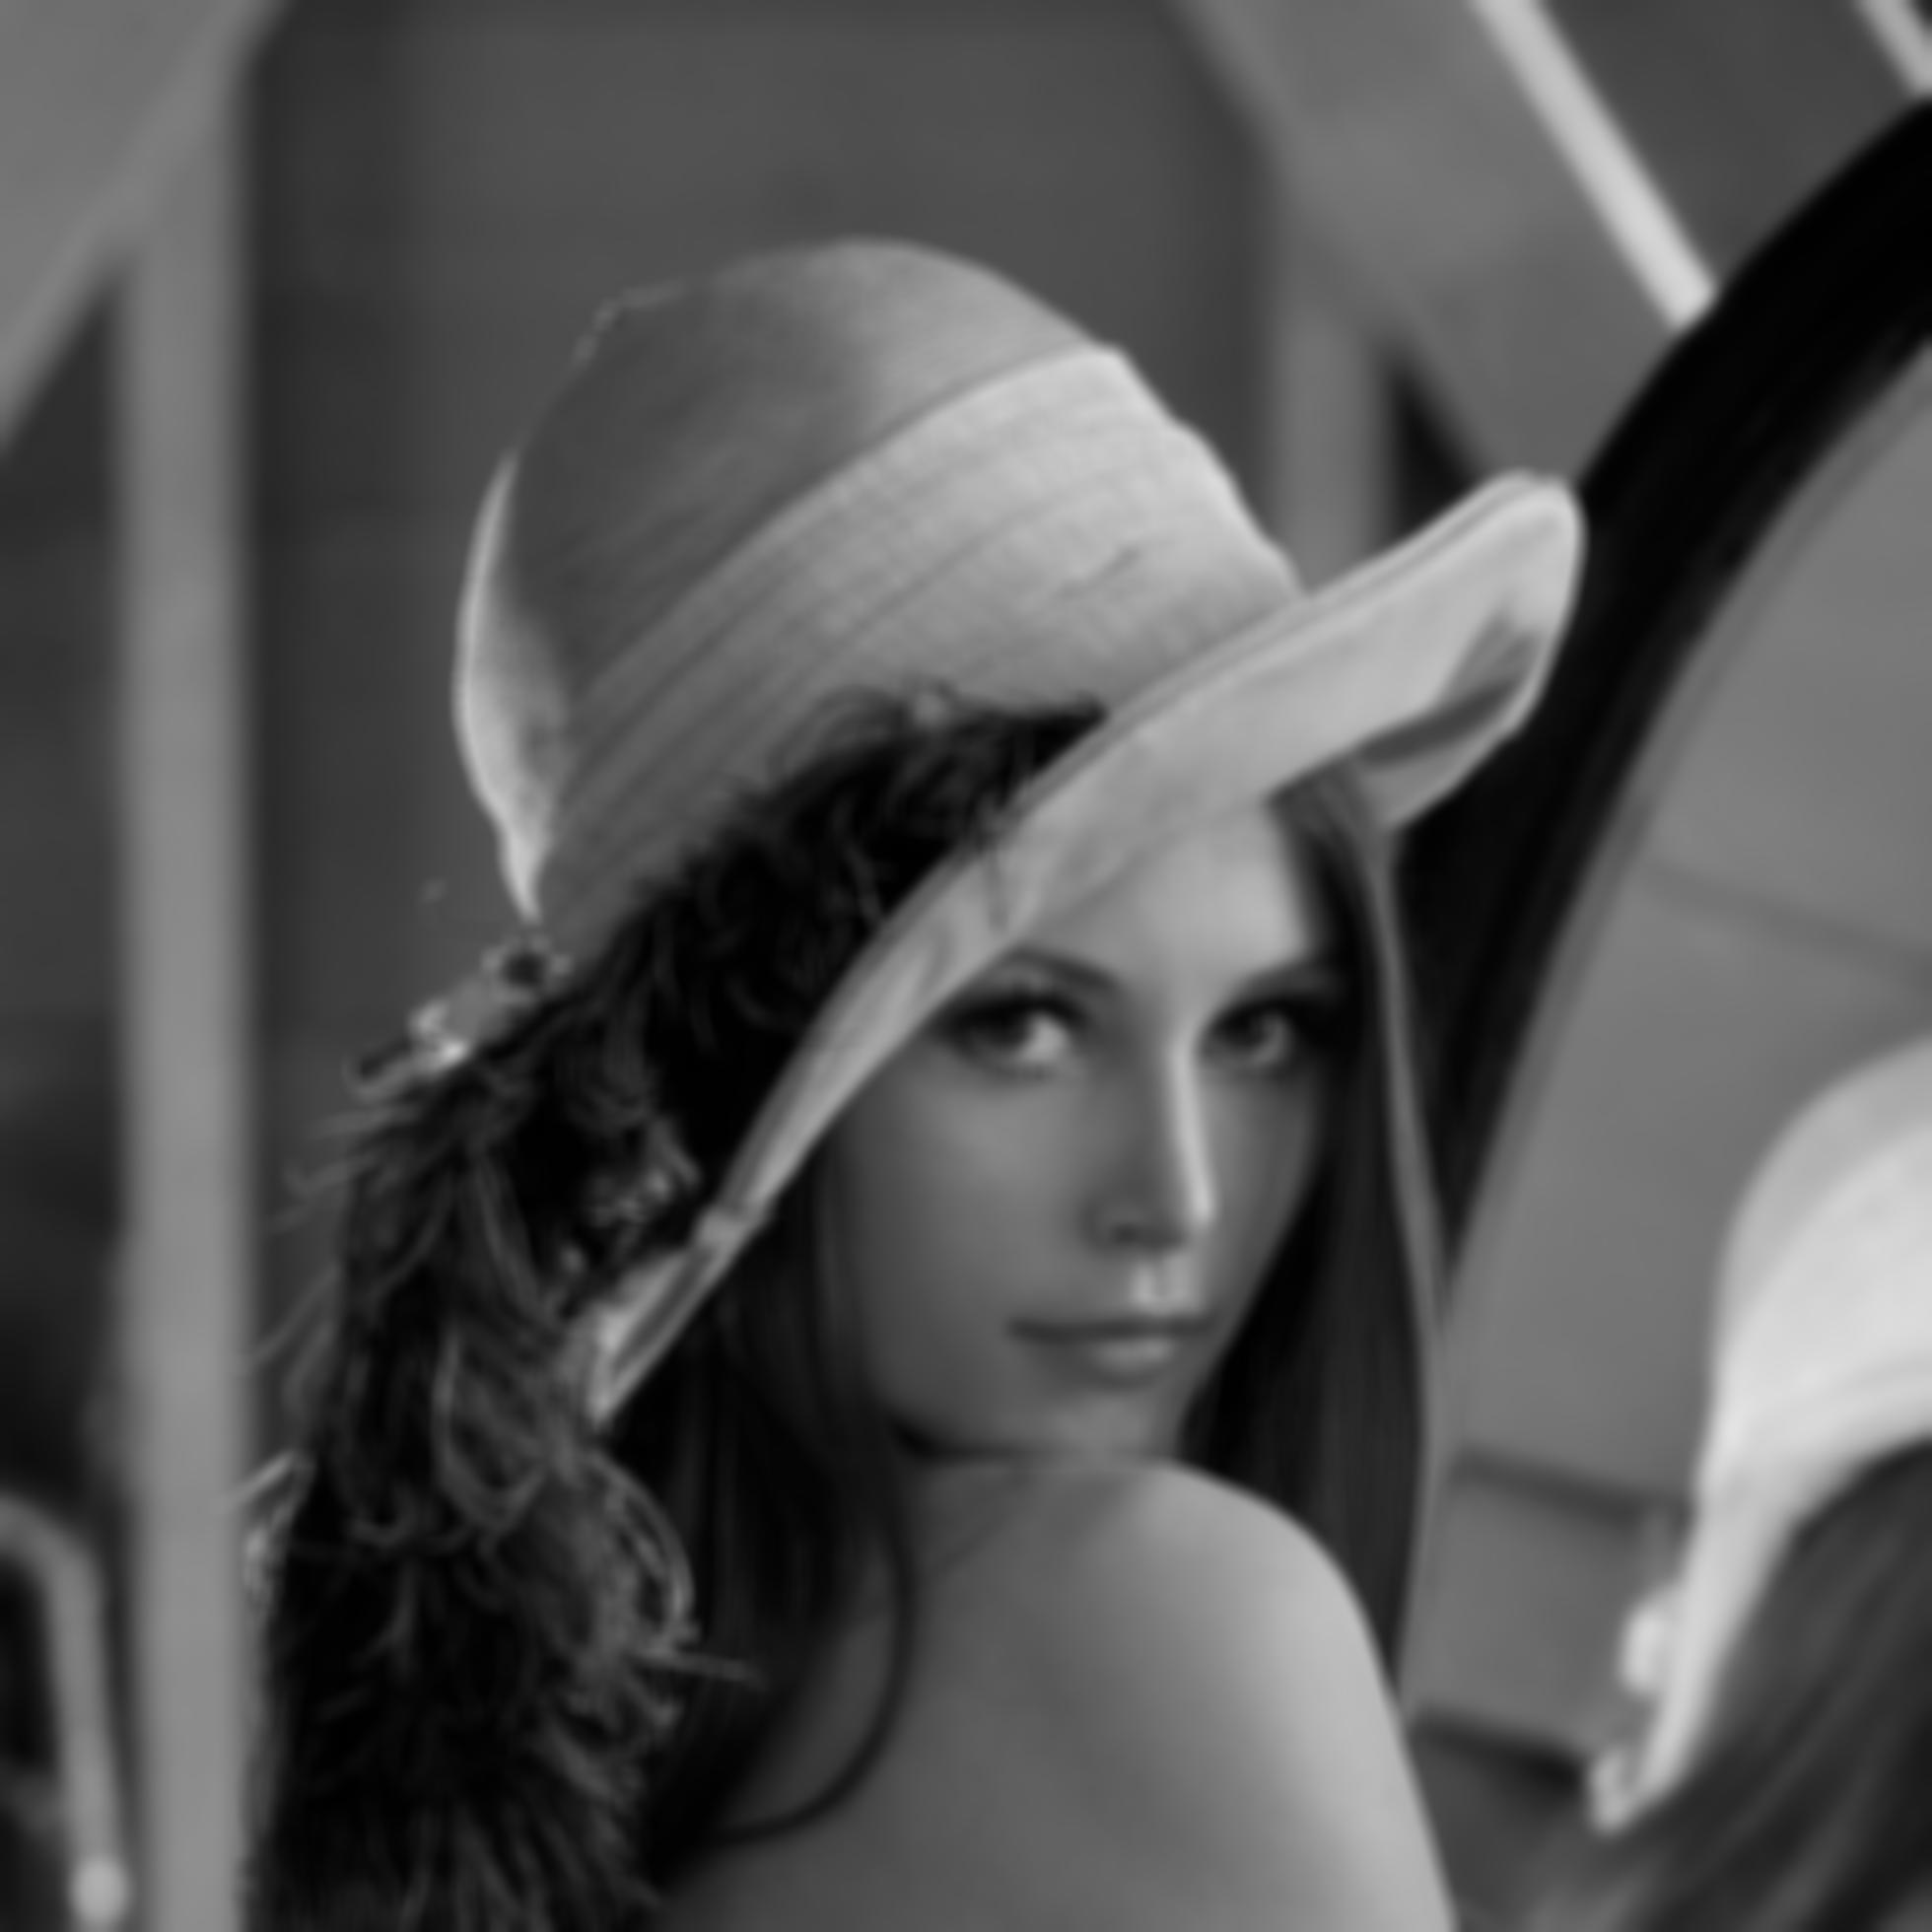
\includegraphics[width=7cm]{resources/modified/lena/lena_blur_20x20.jpg}
\linebreak
\tiny{Wynik działania filtru 20x20}
\end{center}

\begin{center}
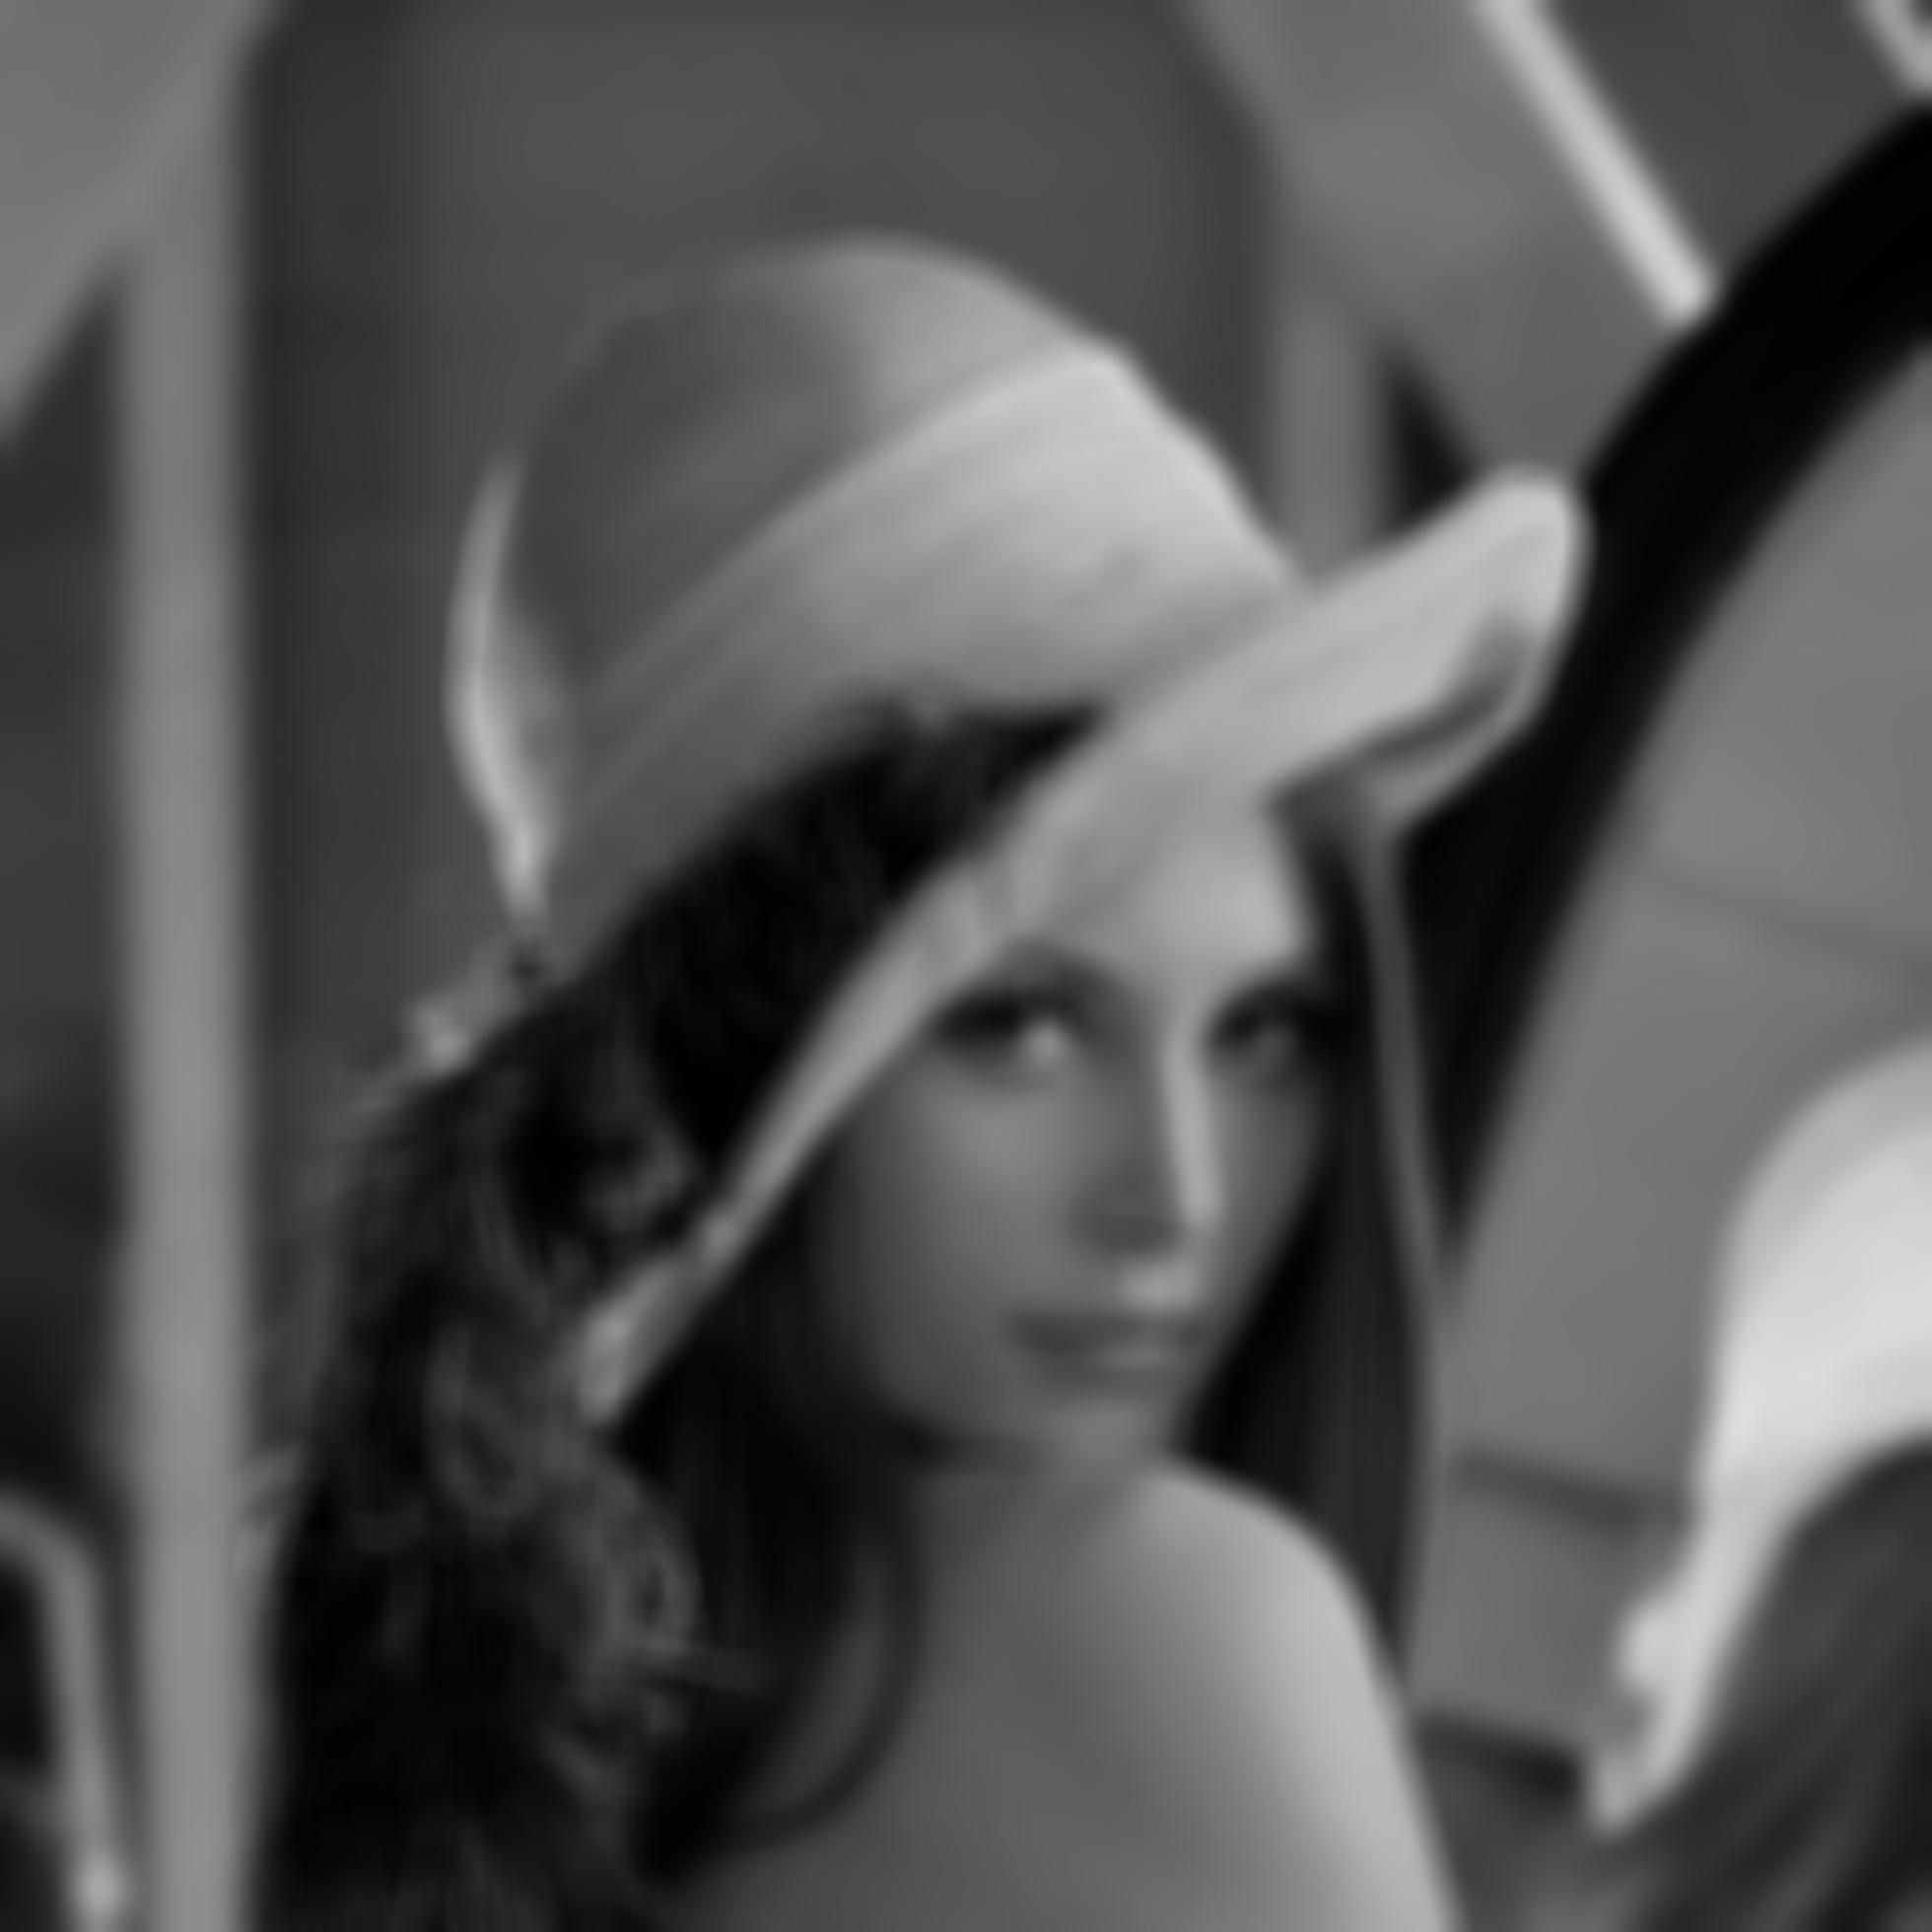
\includegraphics[width=7cm]{resources/modified/lena/lena_blur_40x40.jpg}
\linebreak
\tiny{Wynik działania filtru 40x40}
\end{center}

\pagebreak
\paragraph{\indent Jak można zauważyć na powyższych obrazach, rozmycie w stosunku do obrazu źródłowego jest tym większe, im większe wymiary ma wykorzystana macierz. W filtrach o większej powierzchni na jeden piksel obrazu wyjściowego przypada średnia wartość większej ilości pikseli obrazu źródłowego (np dla filtra 40x40 będzie to 1600 pikseli). Skutkuje to zwiększonym wygładzeniem sygnału, co w tym przypadku oznacza rozmycie obrazu. Poniżej przykład na prostszym obrazie:}

\begin{center}
\text{wyniki działania filtrów 40x40 oraz 20x20:}\\

\includegraphics[width=7cm]{resources/modified/sample/sample_blur_40x40.jpg}

\includegraphics[width=7cm]{resources/modified/sample/sample_blur_20x20.jpg}
\end{center}

\pagebreak
\subsection{Dodatkowe filtry}

\begin{center}
\text{wyniki działania filtrów 3x40 oraz 40x3:}\\
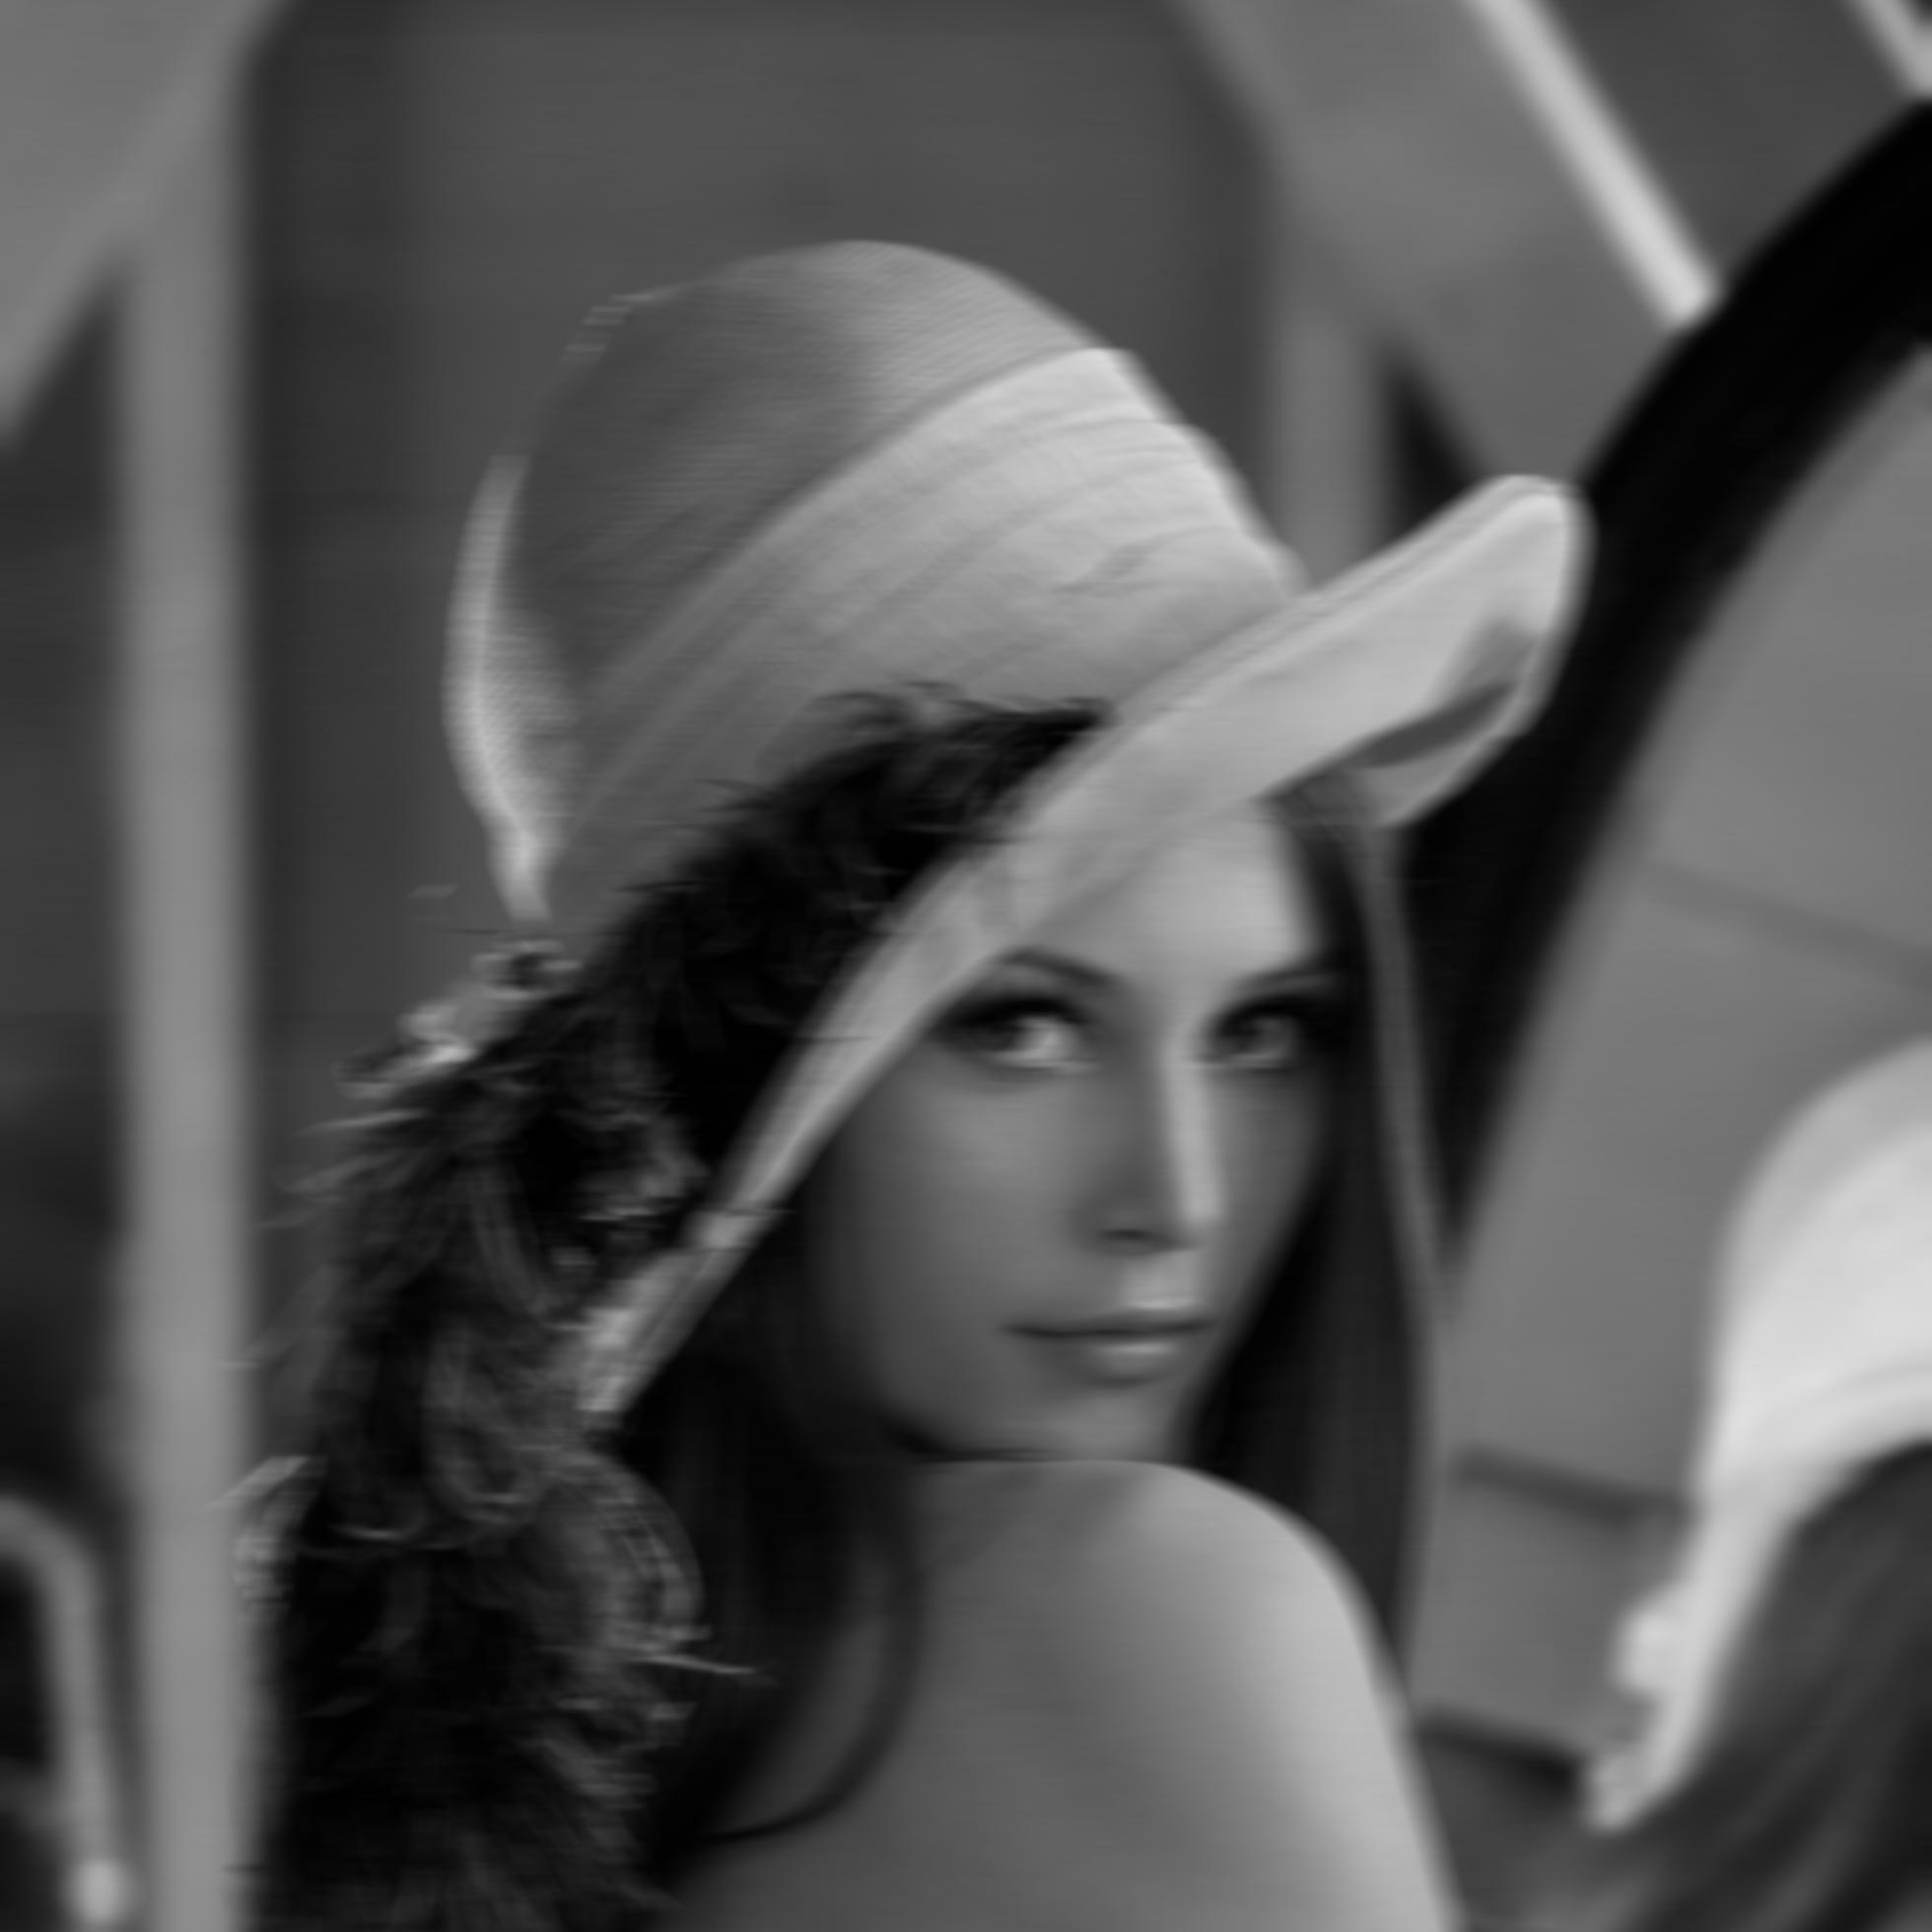
\includegraphics[width=7cm]{resources/modified/lena/lena_blur_3x40.jpg}
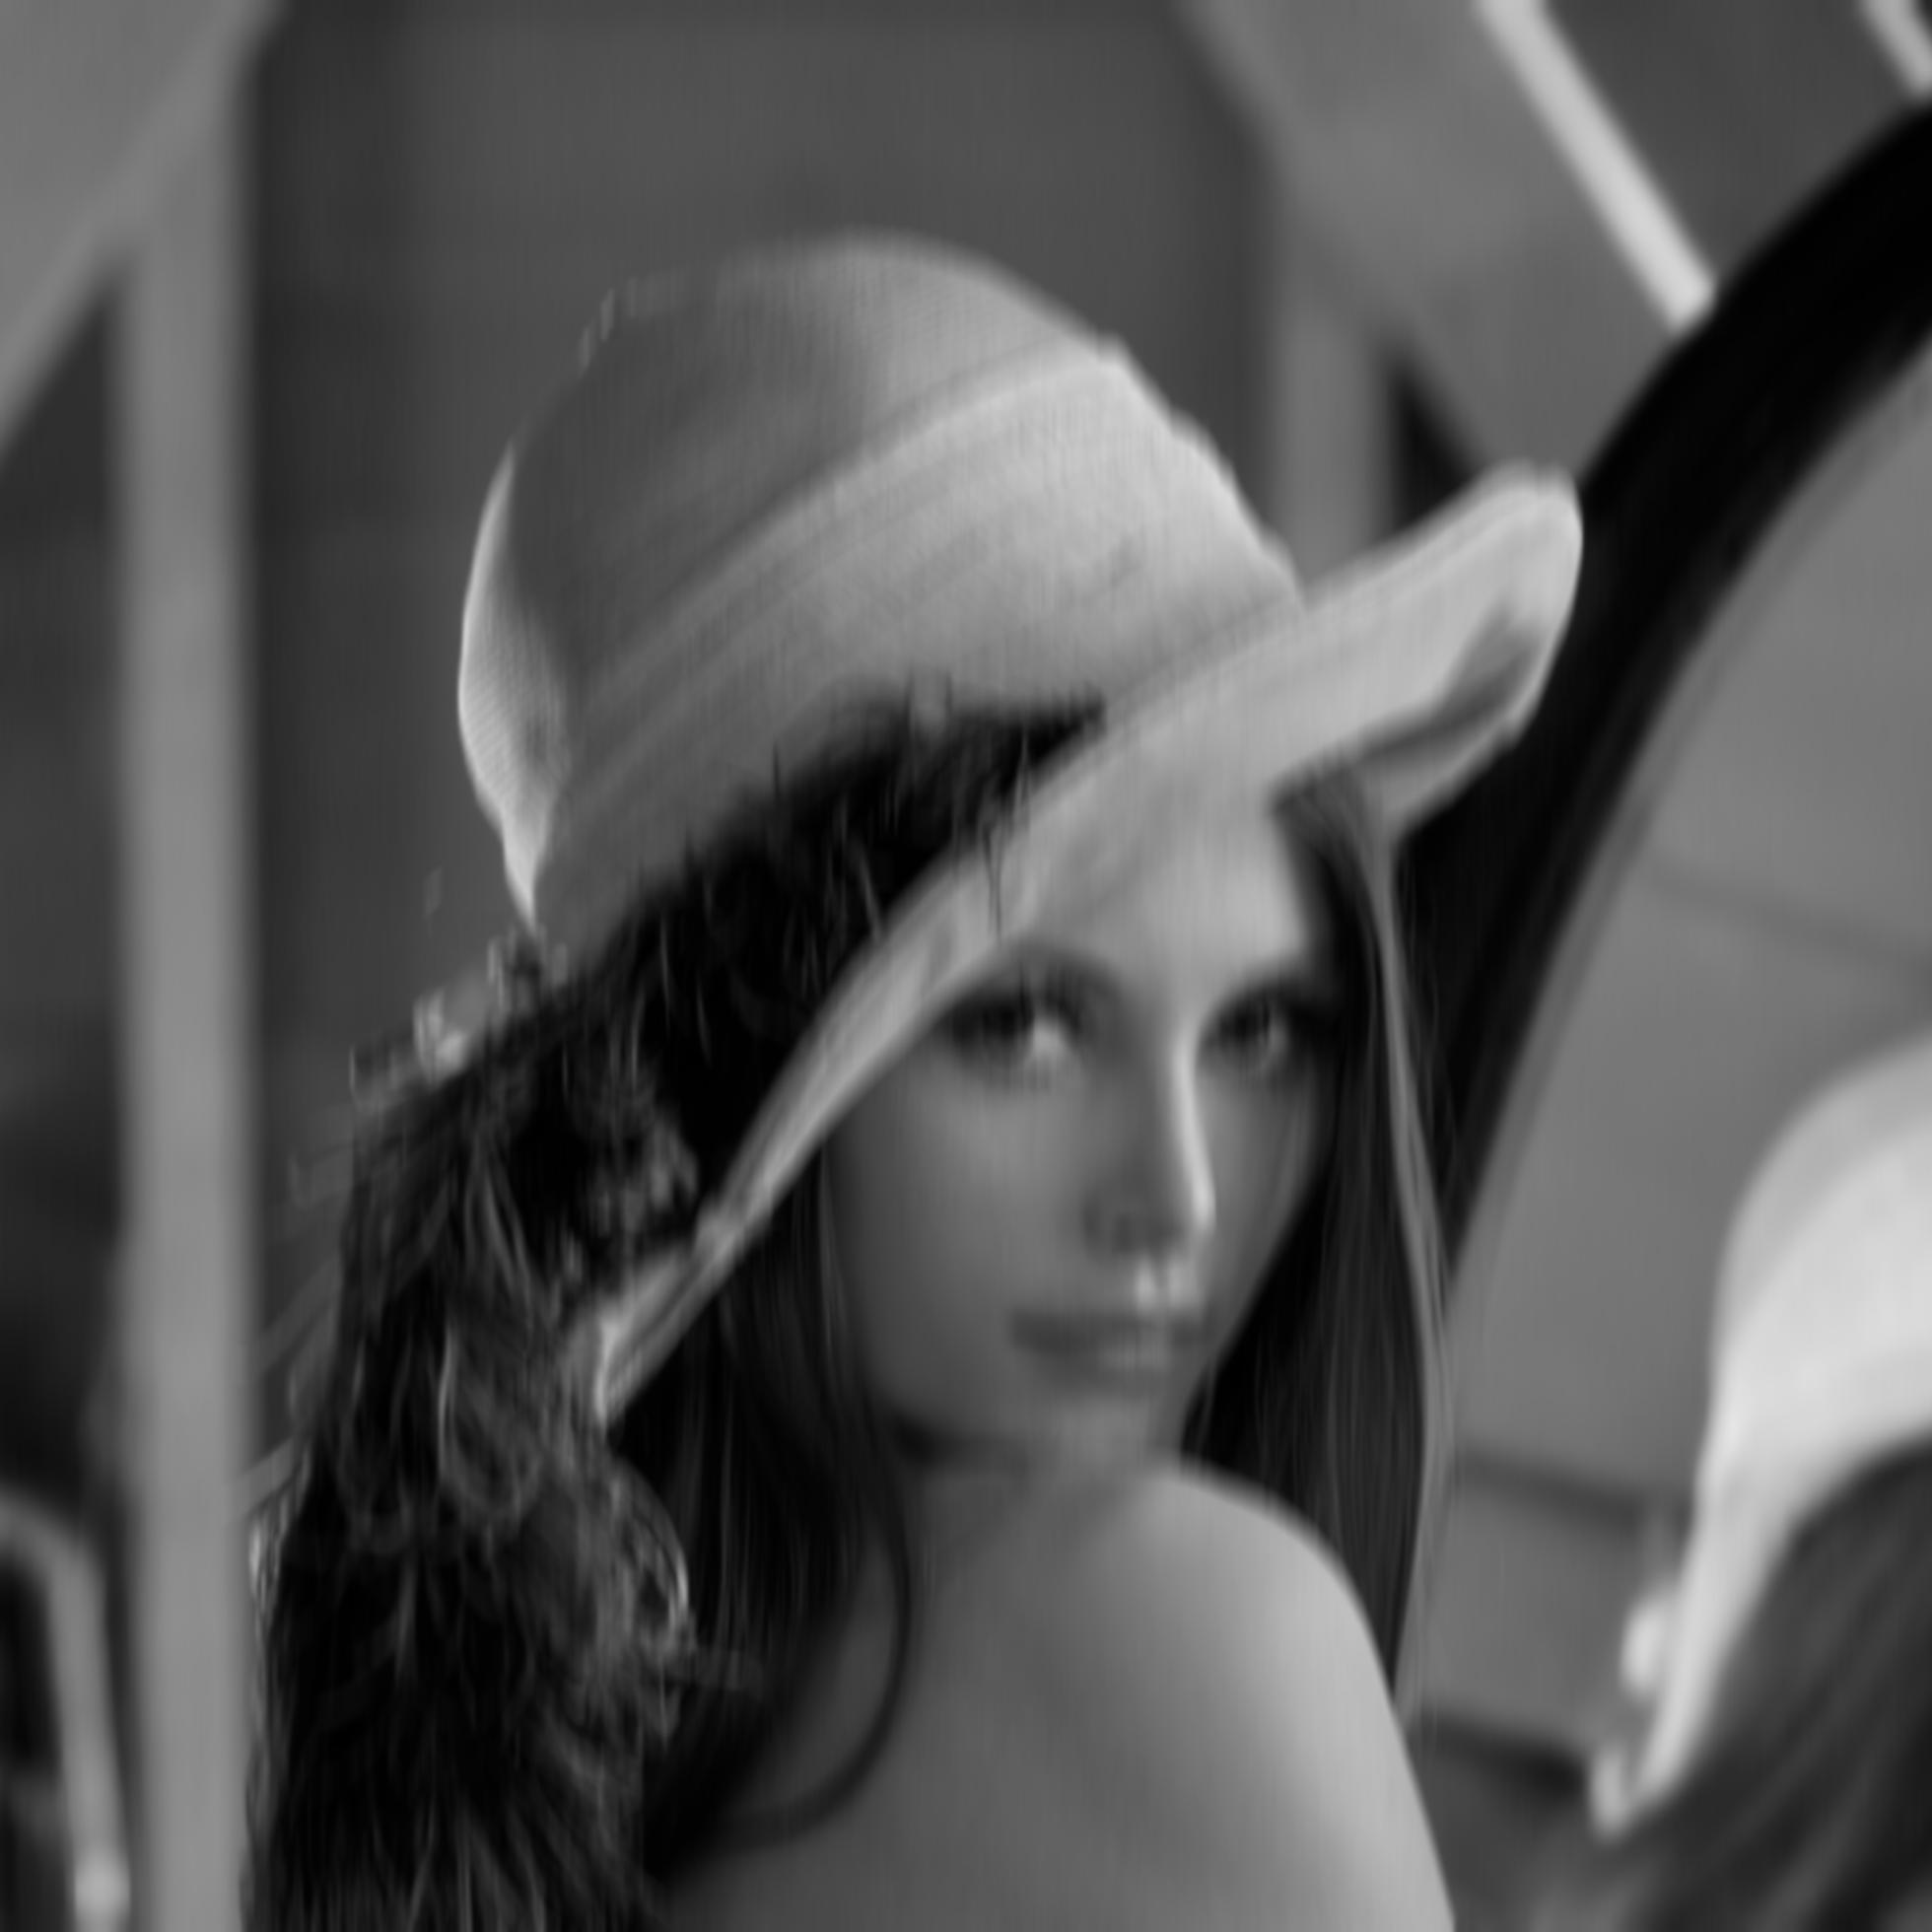
\includegraphics[width=7cm]{resources/modified/lena/lena_blur_40x3.jpg}
\\
\text{wyniki działania filtrów 20x3 oraz 3x20:}\\
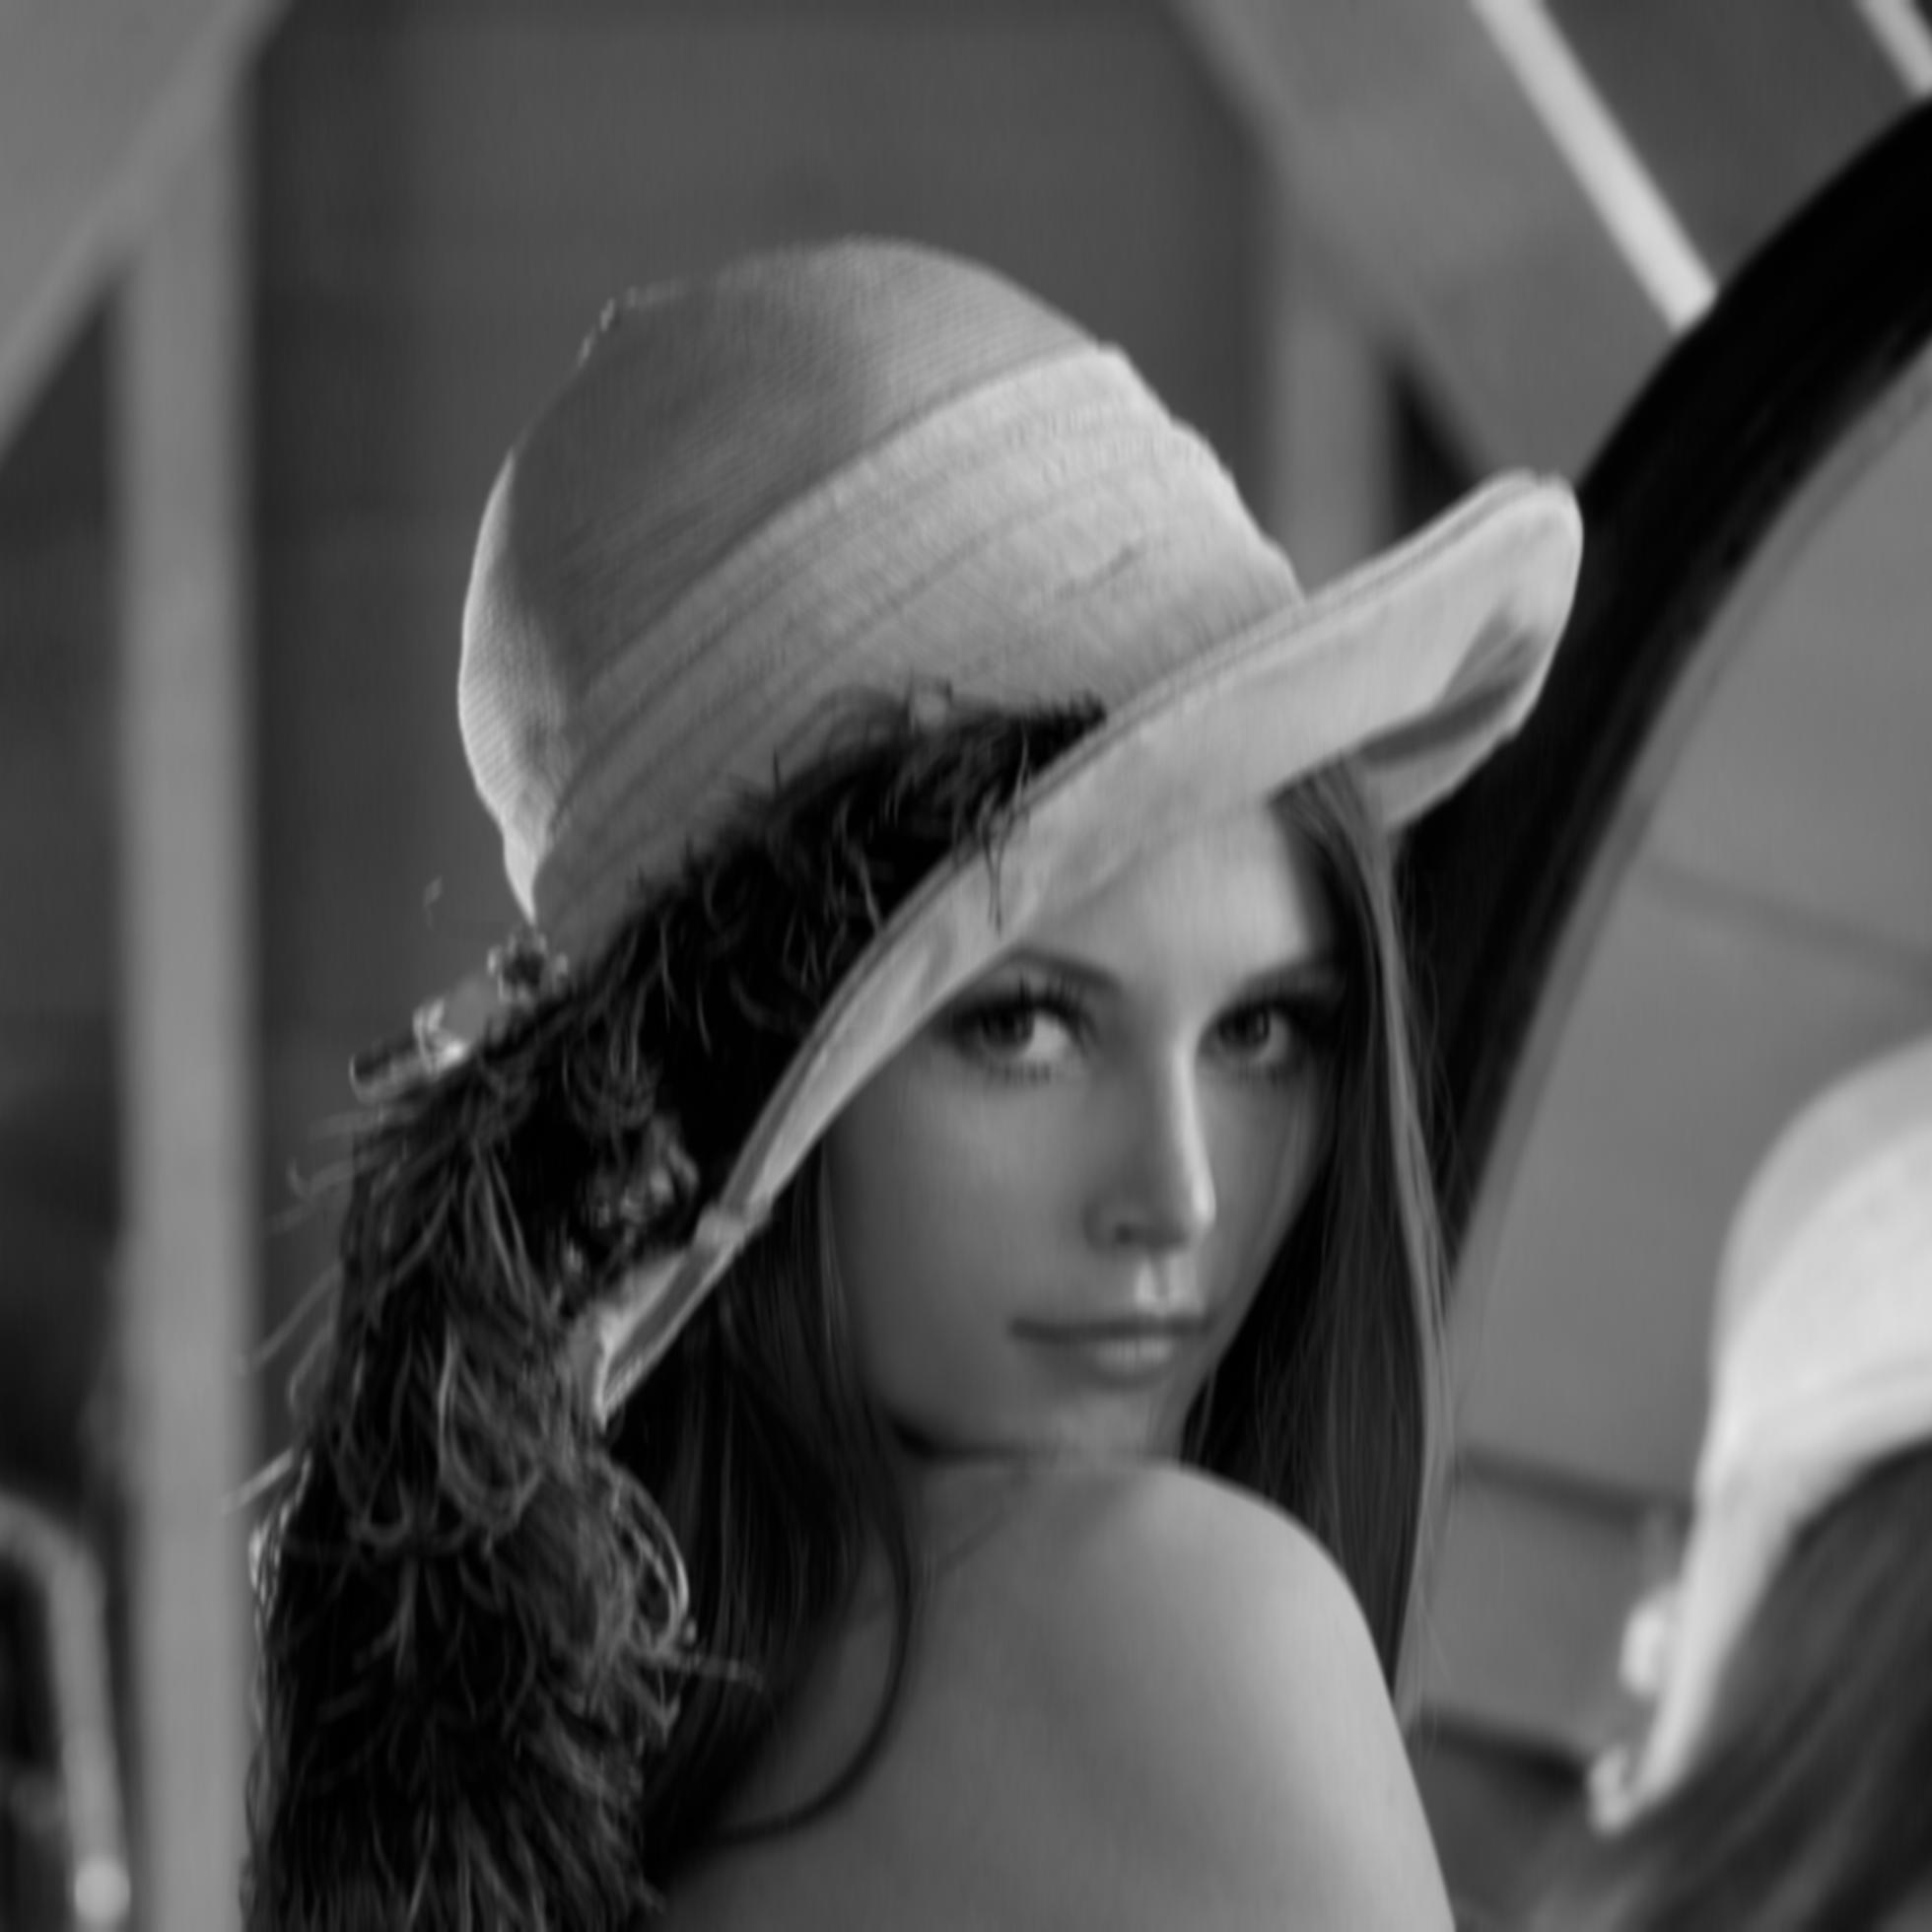
\includegraphics[width=7cm]{resources/modified/lena/lena_blur_20x3.jpg}
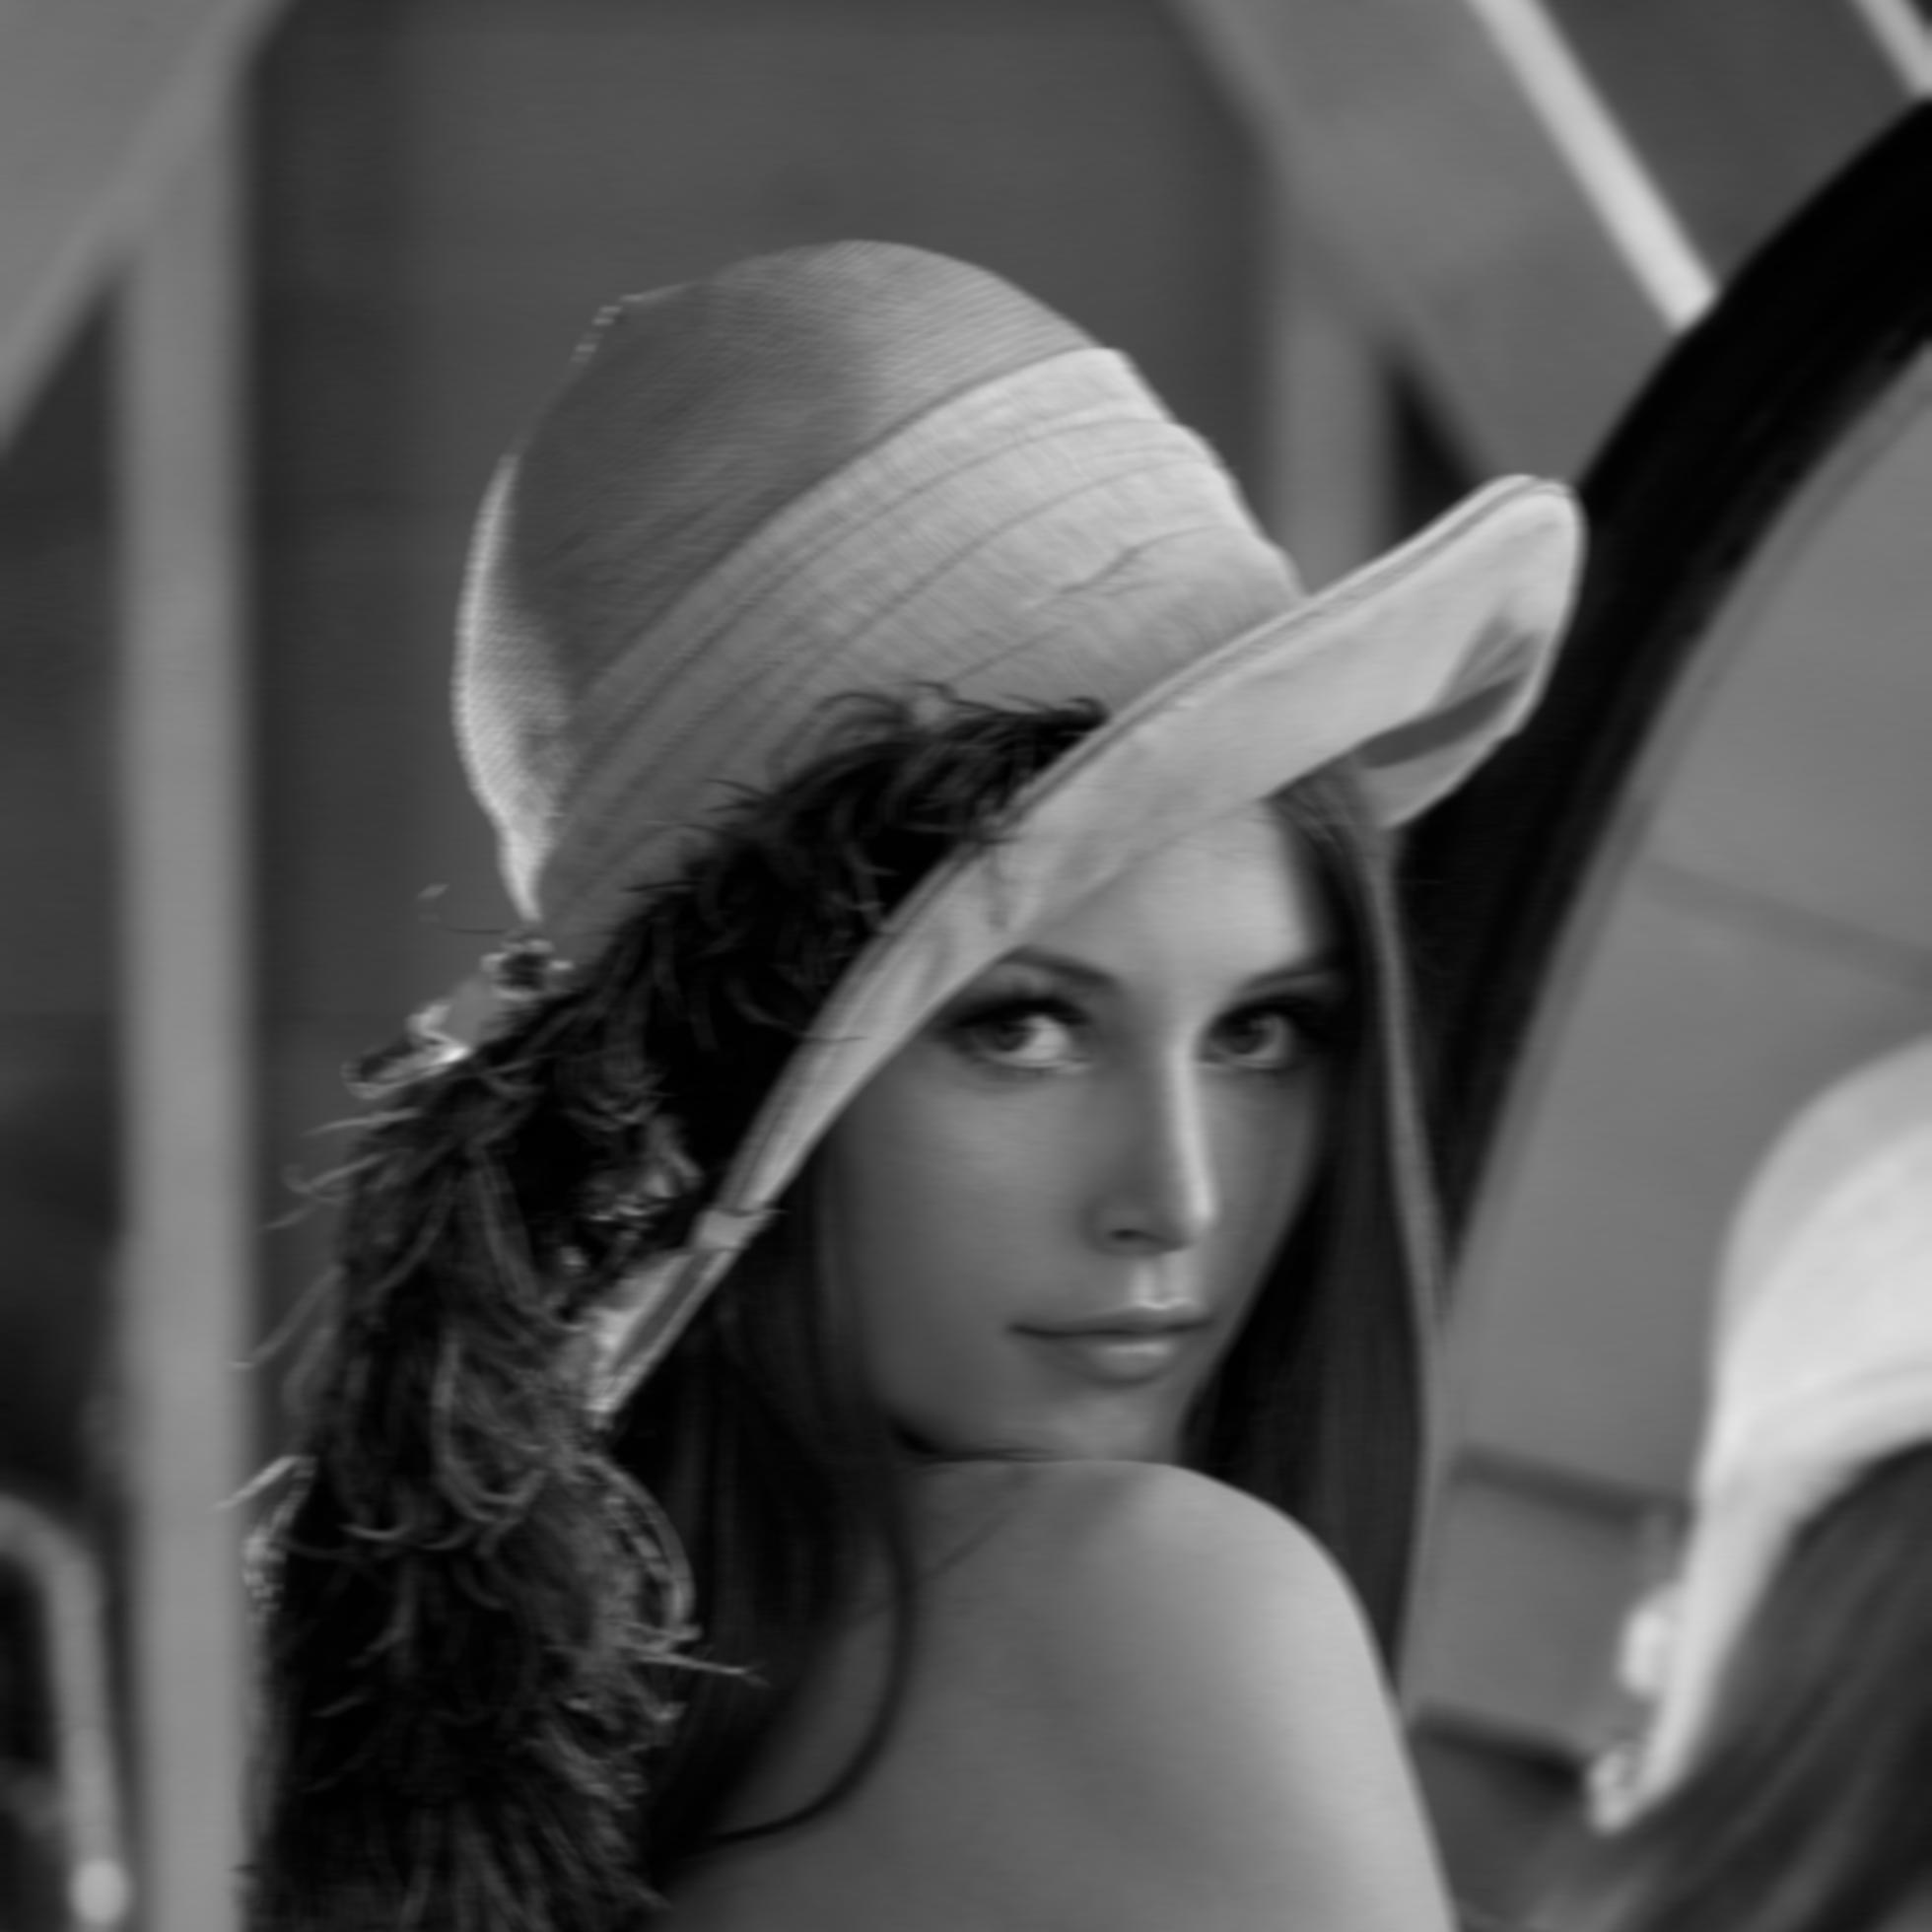
\includegraphics[width=7cm]{resources/modified/lena/lena_blur_3x20.jpg}
\\
\text{wyniki działania filtrów 40x3 oraz 40x5:}\\
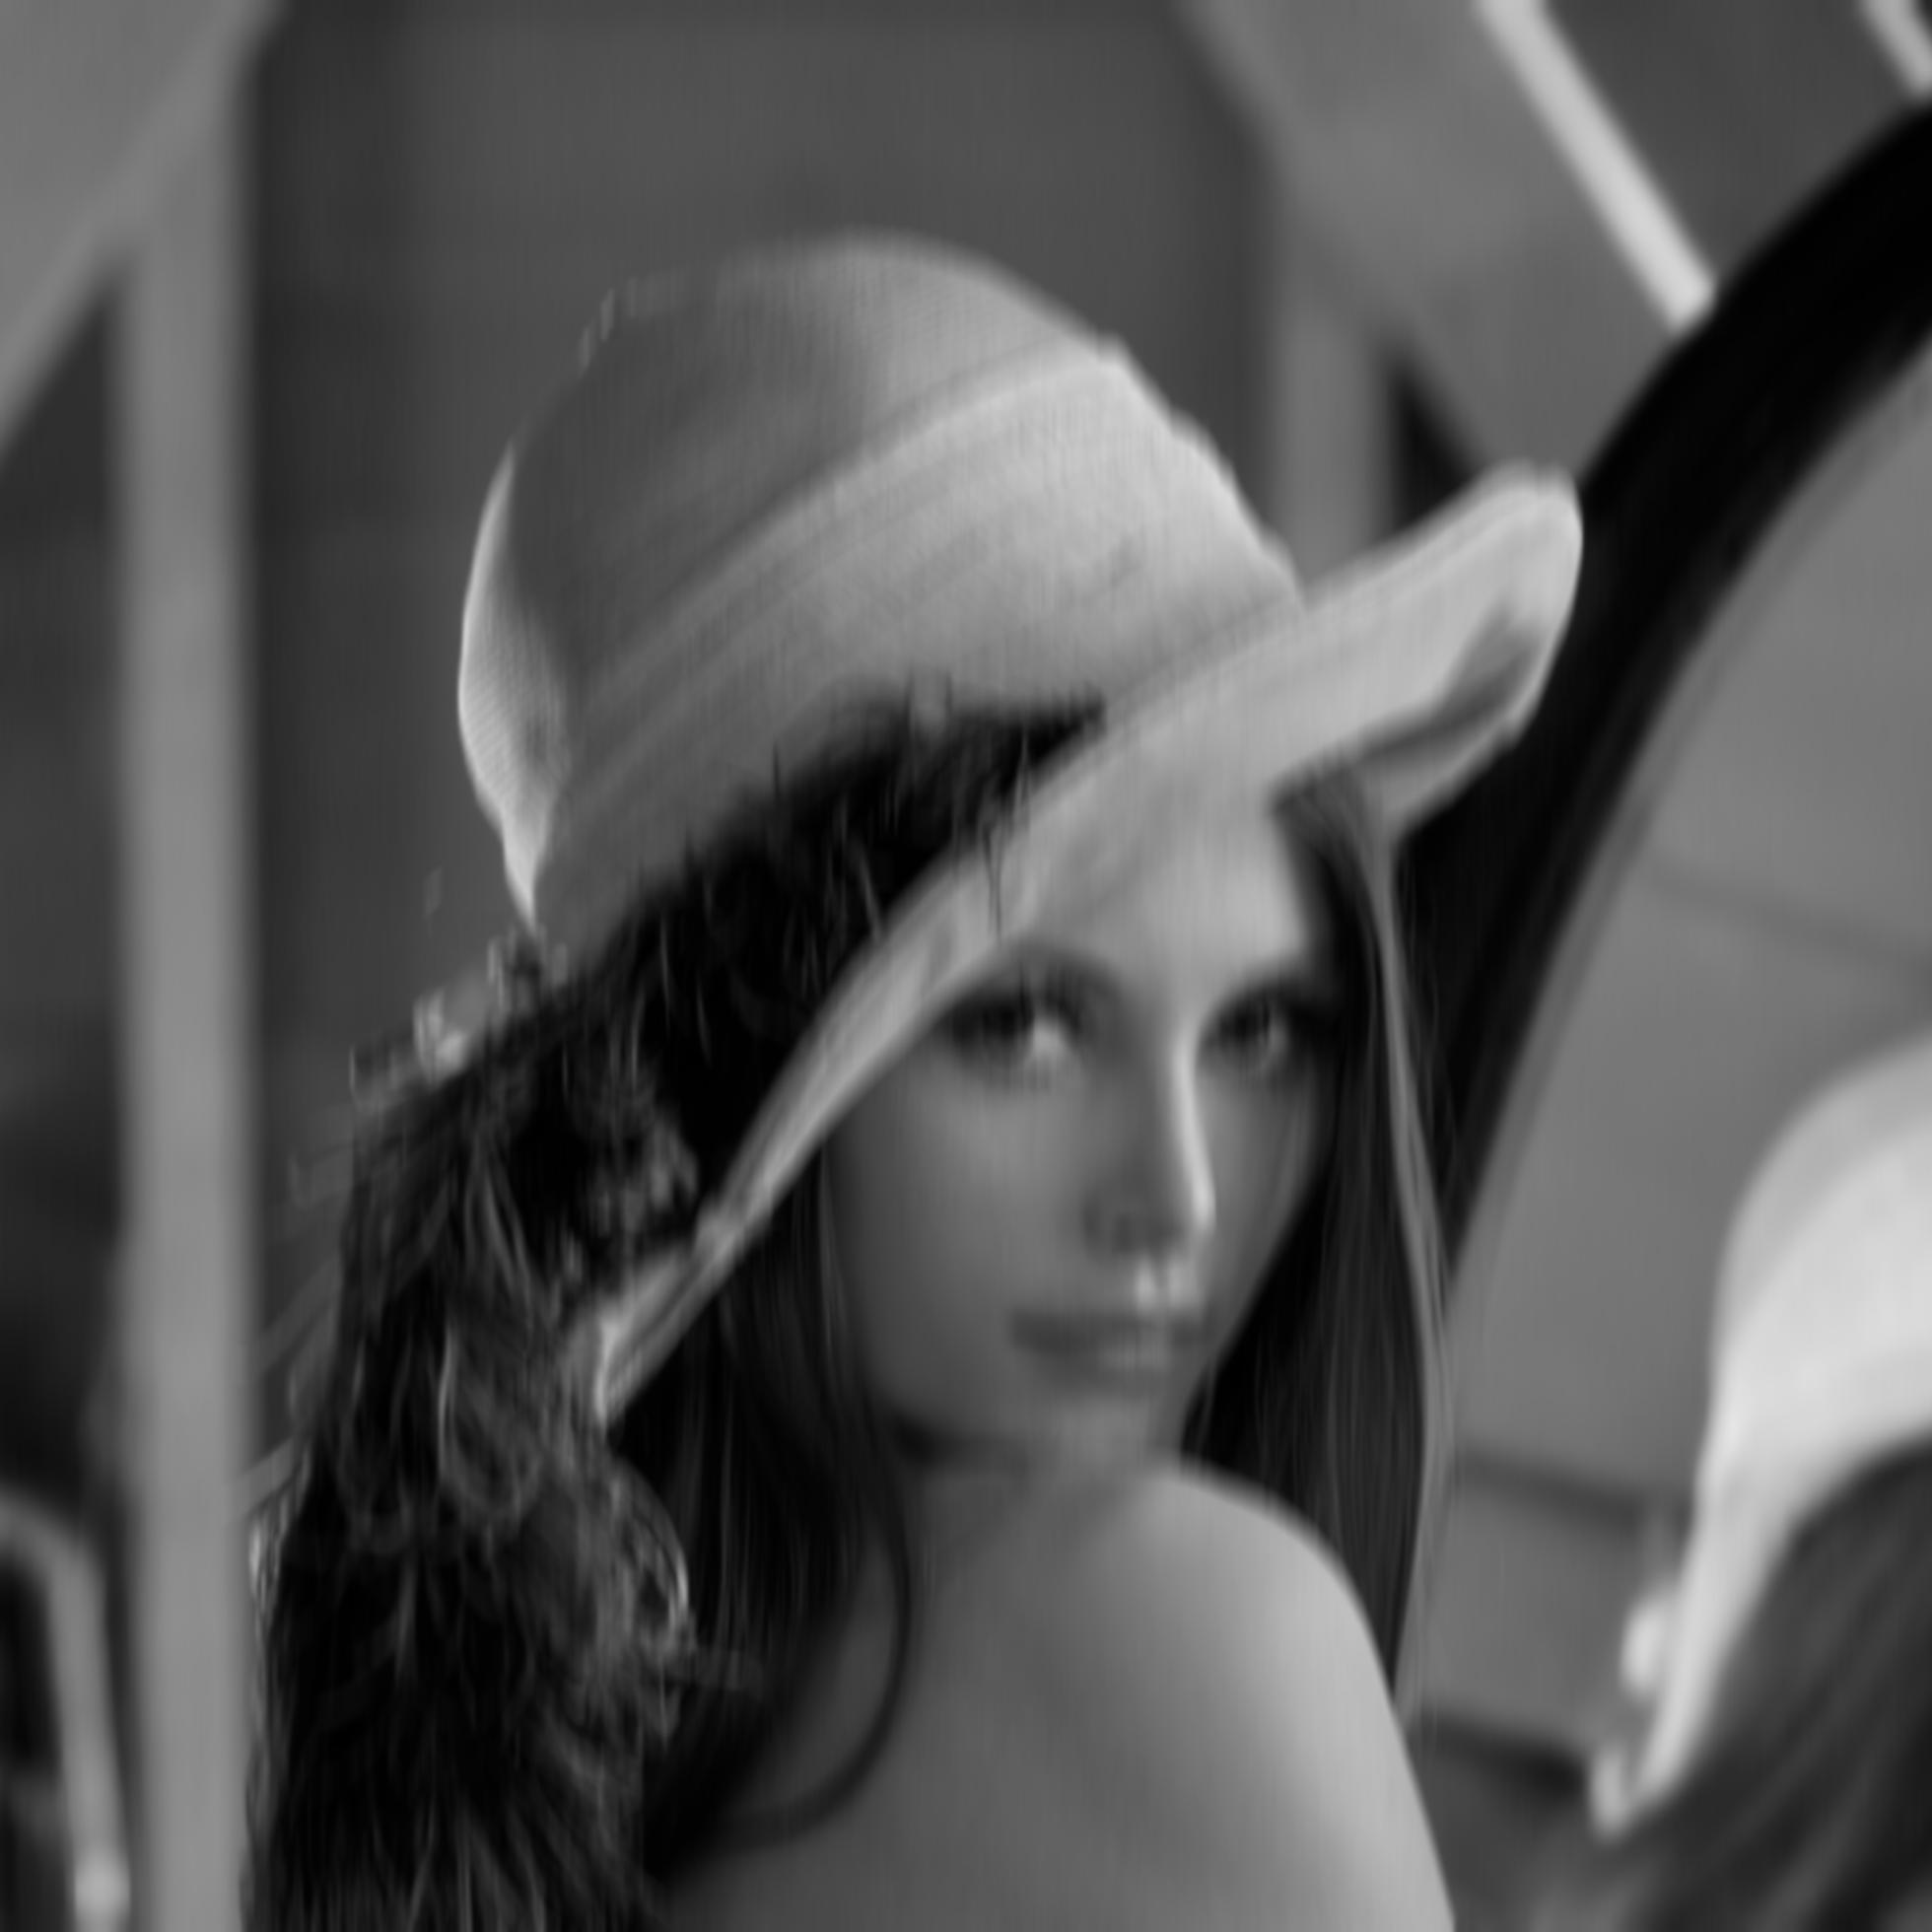
\includegraphics[width=7cm]{resources/modified/lena/lena_blur_40x3.jpg}
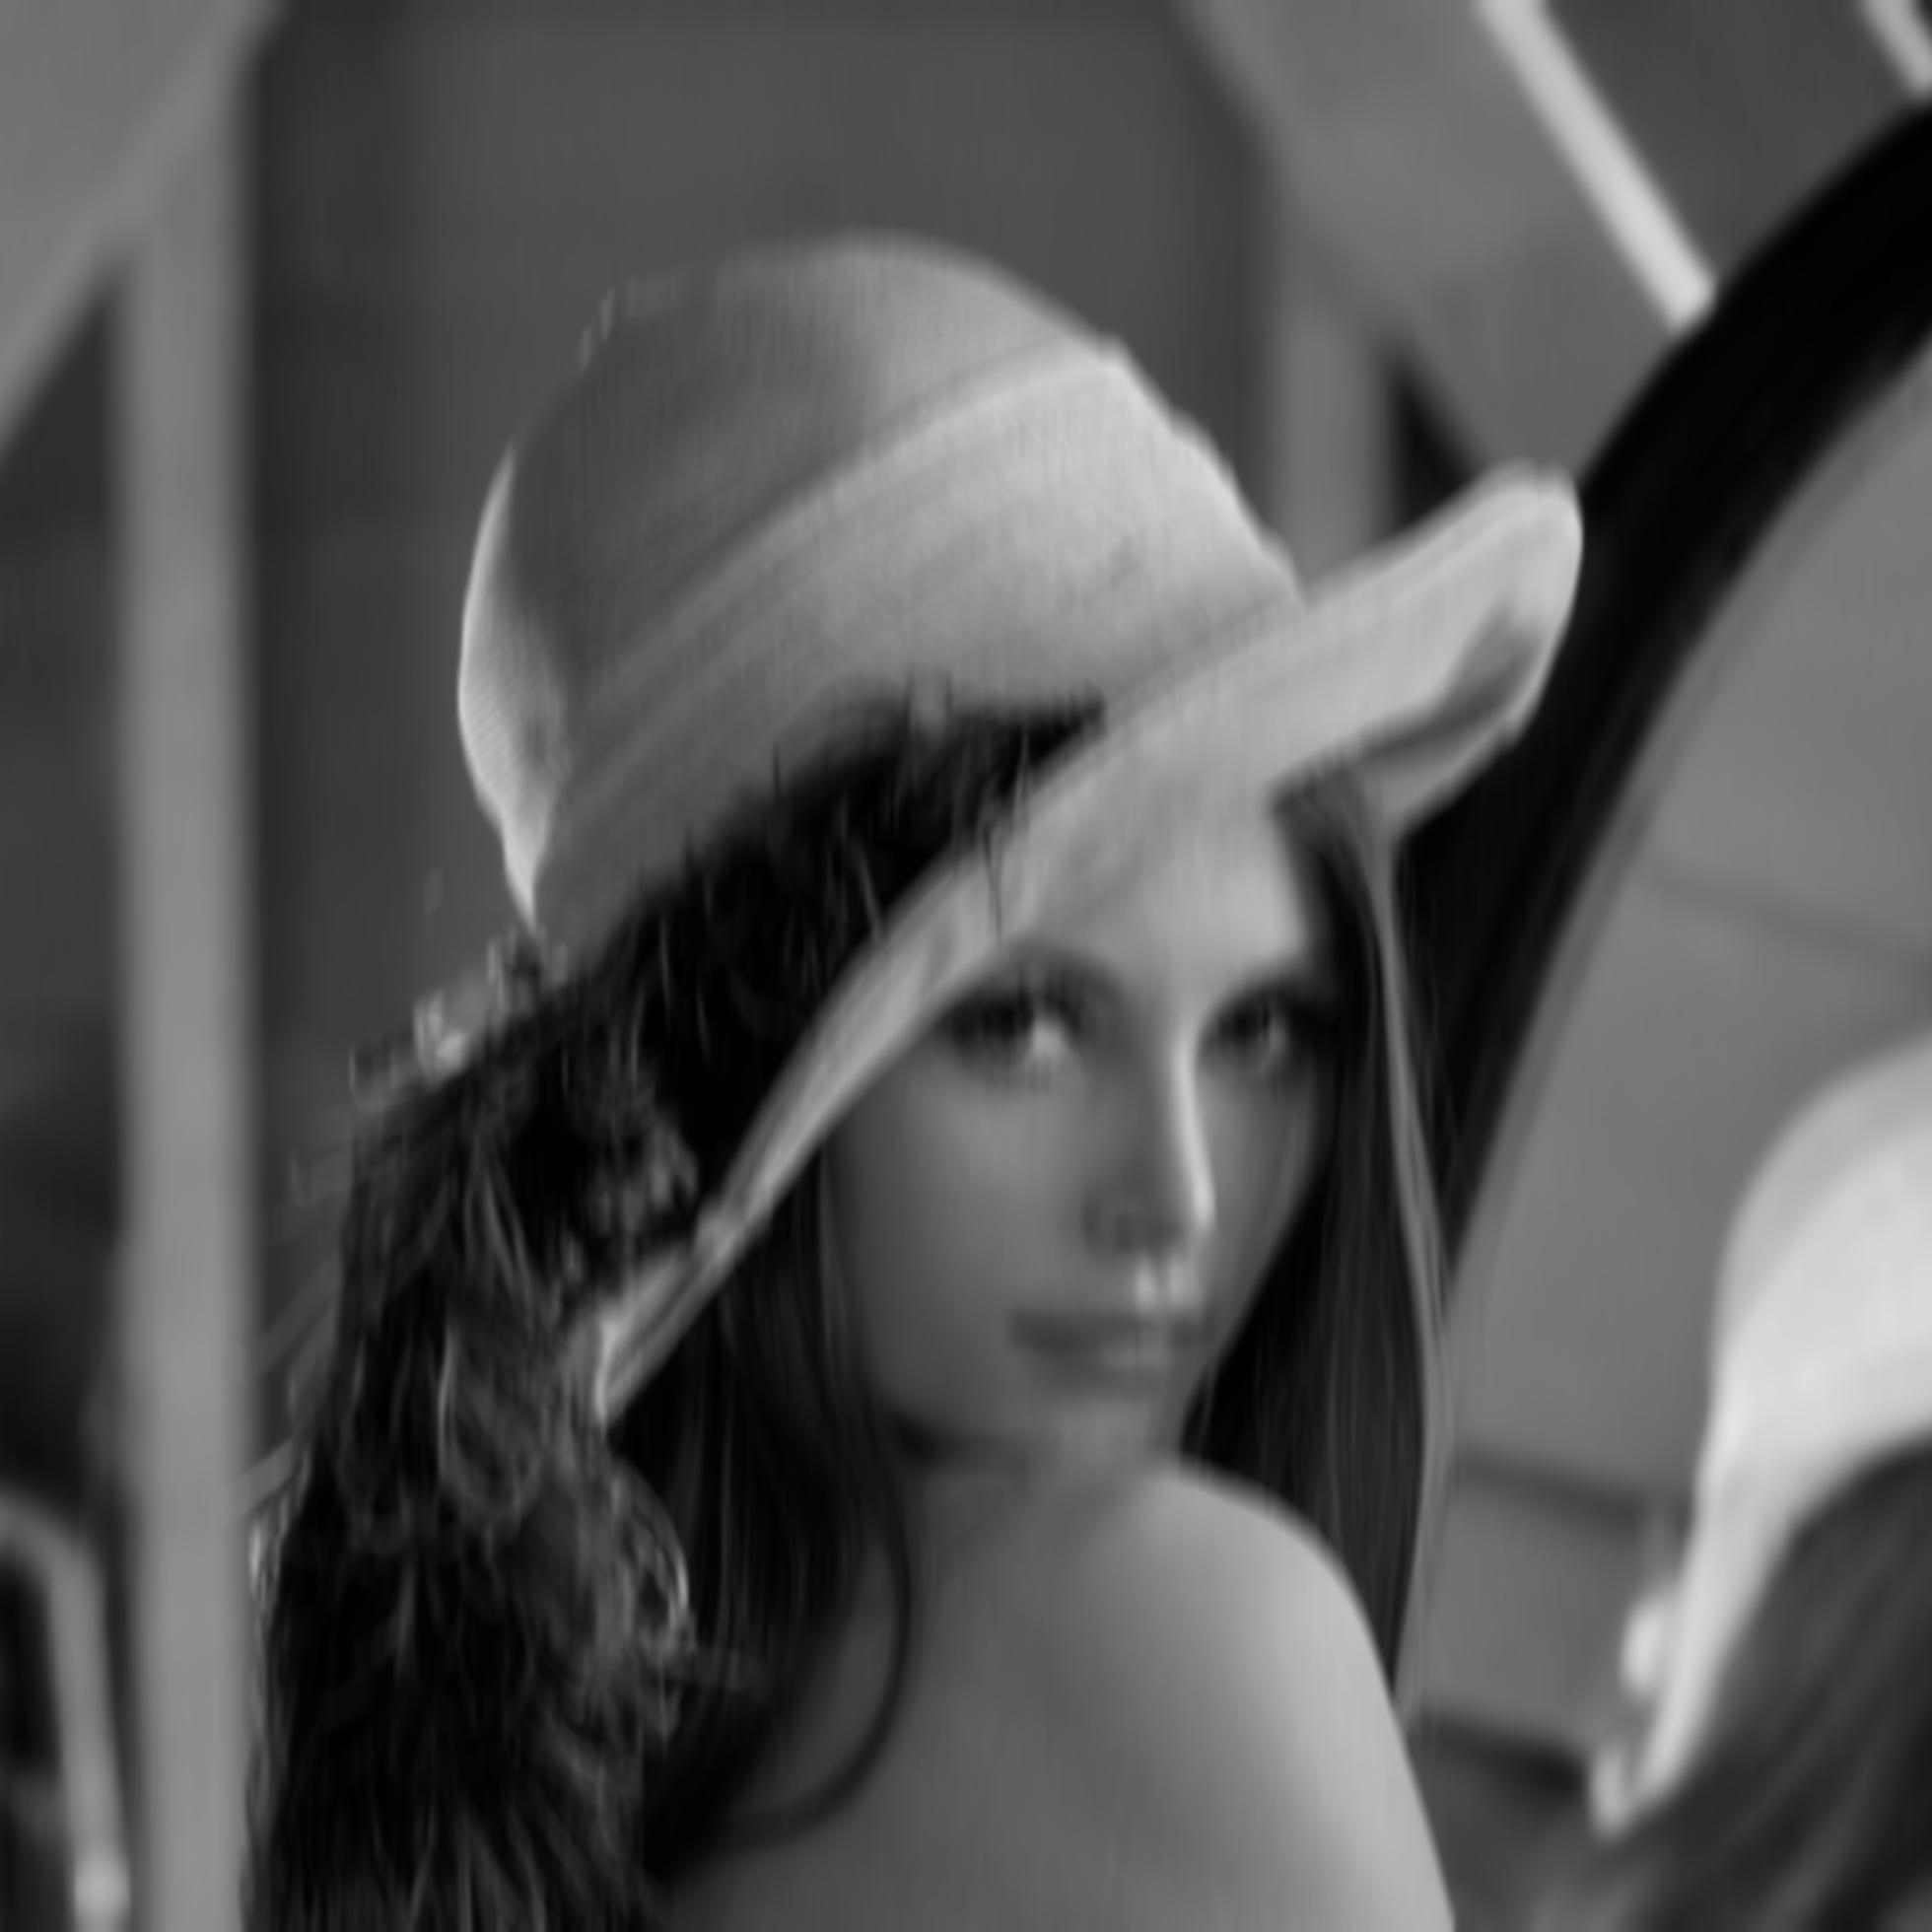
\includegraphics[width=7cm]{resources/modified/lena/lena_blur_40x5.jpg}
\end{center}

\pagebreak
\paragraph{\indent Dodatkowym zjawiskiem powstającym tylko dla niektórych filtrów (nie kwadratowych) jest zwiększone rozmycie wzdłuż jednej z osi. Jeśli filtr ma szerokość większą niż wysokość obraz zostanie bardziej rozmyty w osi poziomek. Jeśli filtr ma wysokość większą niż szerokość obraz zostanie bardziej rozmyty w osi pionowej. Im większy jest stosunek wysokości do szerokości tym efekt ten będzie bardziej wyraźny. Wynika to z faktu, że do kolejnych pikseli obrazu wyjściowego trafia więcej danych z jego 'sąsiadów' wzdłuż danej osi. Poniżej przykład na prostszym obrazie:}

\begin{center}
\text{wyniki działania filtrów 40x1 oraz 1x40:}\\

\includegraphics[width=7cm]{resources/modified/sample/sample_blur_40x1.jpg}

\includegraphics[width=7cm]{resources/modified/sample/sample_blur_1x40.jpg}
\\
\text{wyniki działania filtrów 40x5 oraz 5x40:}\\

\includegraphics[width=7cm]{resources/modified/sample/sample_blur_40x5.jpg}

\includegraphics[width=7cm]{resources/modified/sample/sample_blur_5x40.jpg}
\end{center}

%%%%%%%%%%%%%%%%%%%%%%%%%%%%%%%%%%%%%%%%%%%%%%%%%%%%%%%%%%%%%%%%%%%%%%%%%%%%%%%%%%%%%%%%%%%%%%%%%%%%%%%%%%%%%%%%%%%%%%%
\pagebreak
\section{Filtr wyostrzający}

\begin{center}
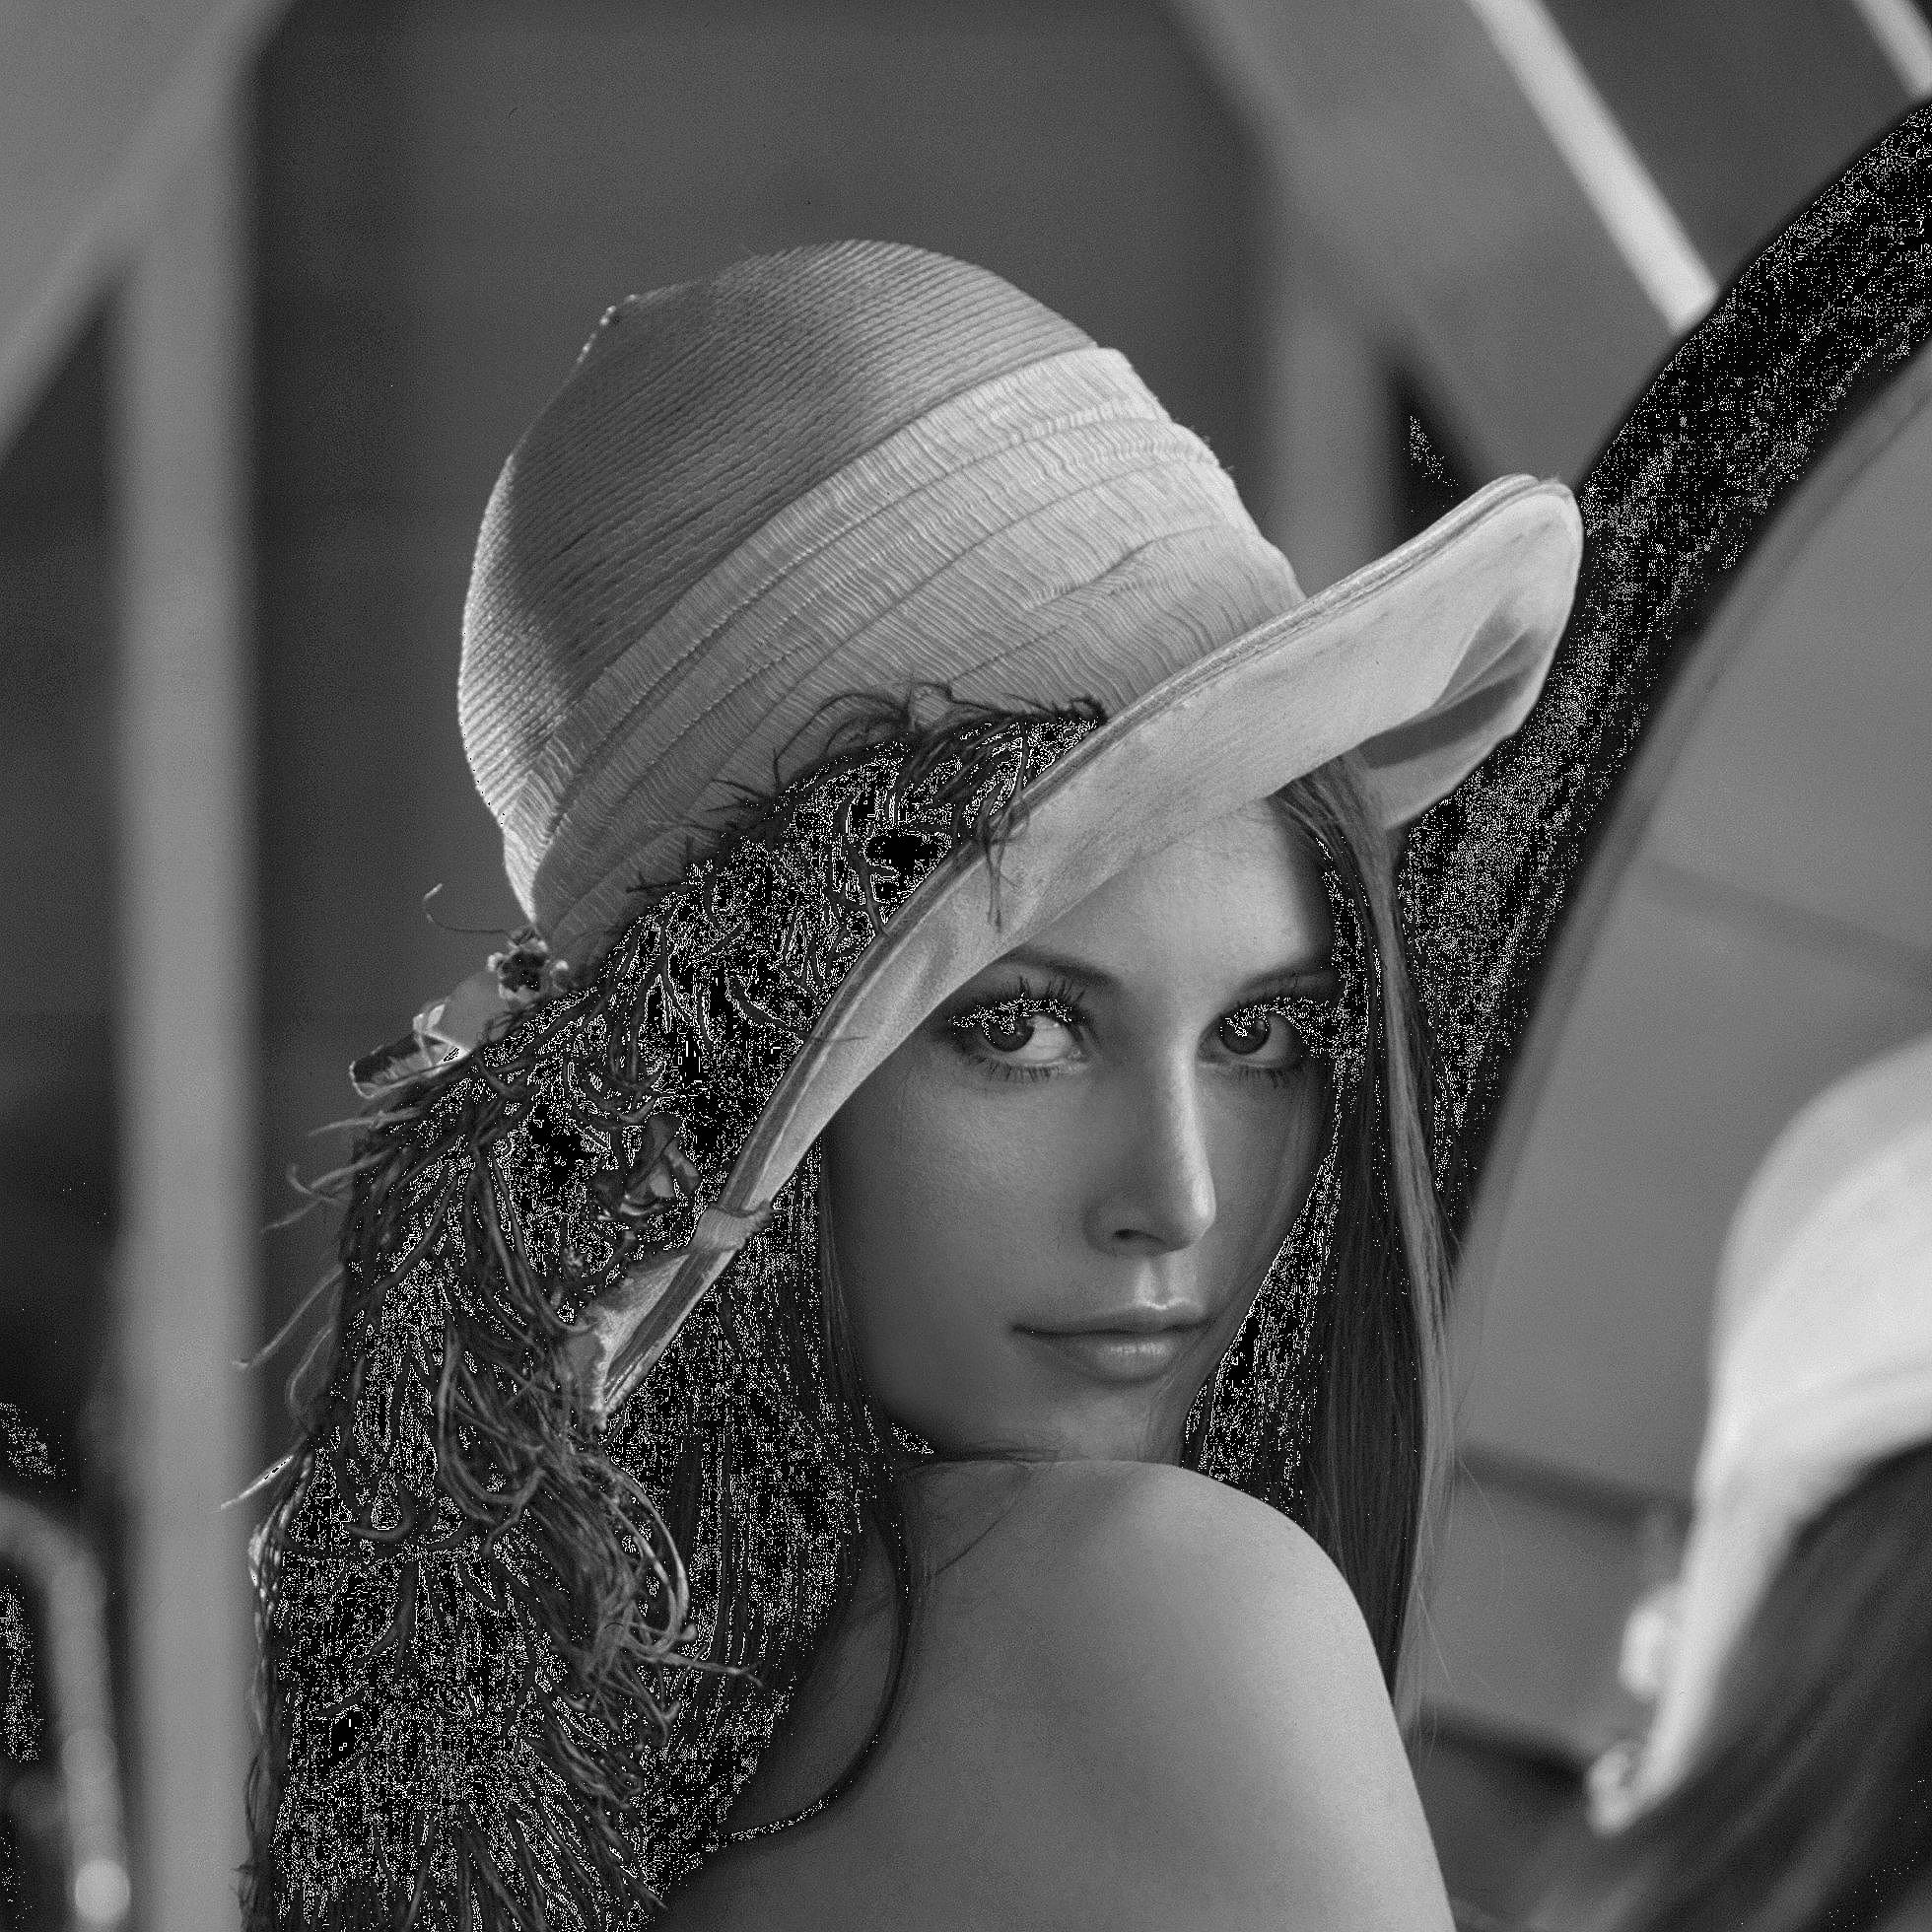
\includegraphics[width=7cm]{resources/modified/lena/lena_sharpen_3x3.jpg}
\linebreak
\tiny{Wynik działania filtru 3x3}
\end{center}

\begin{center}
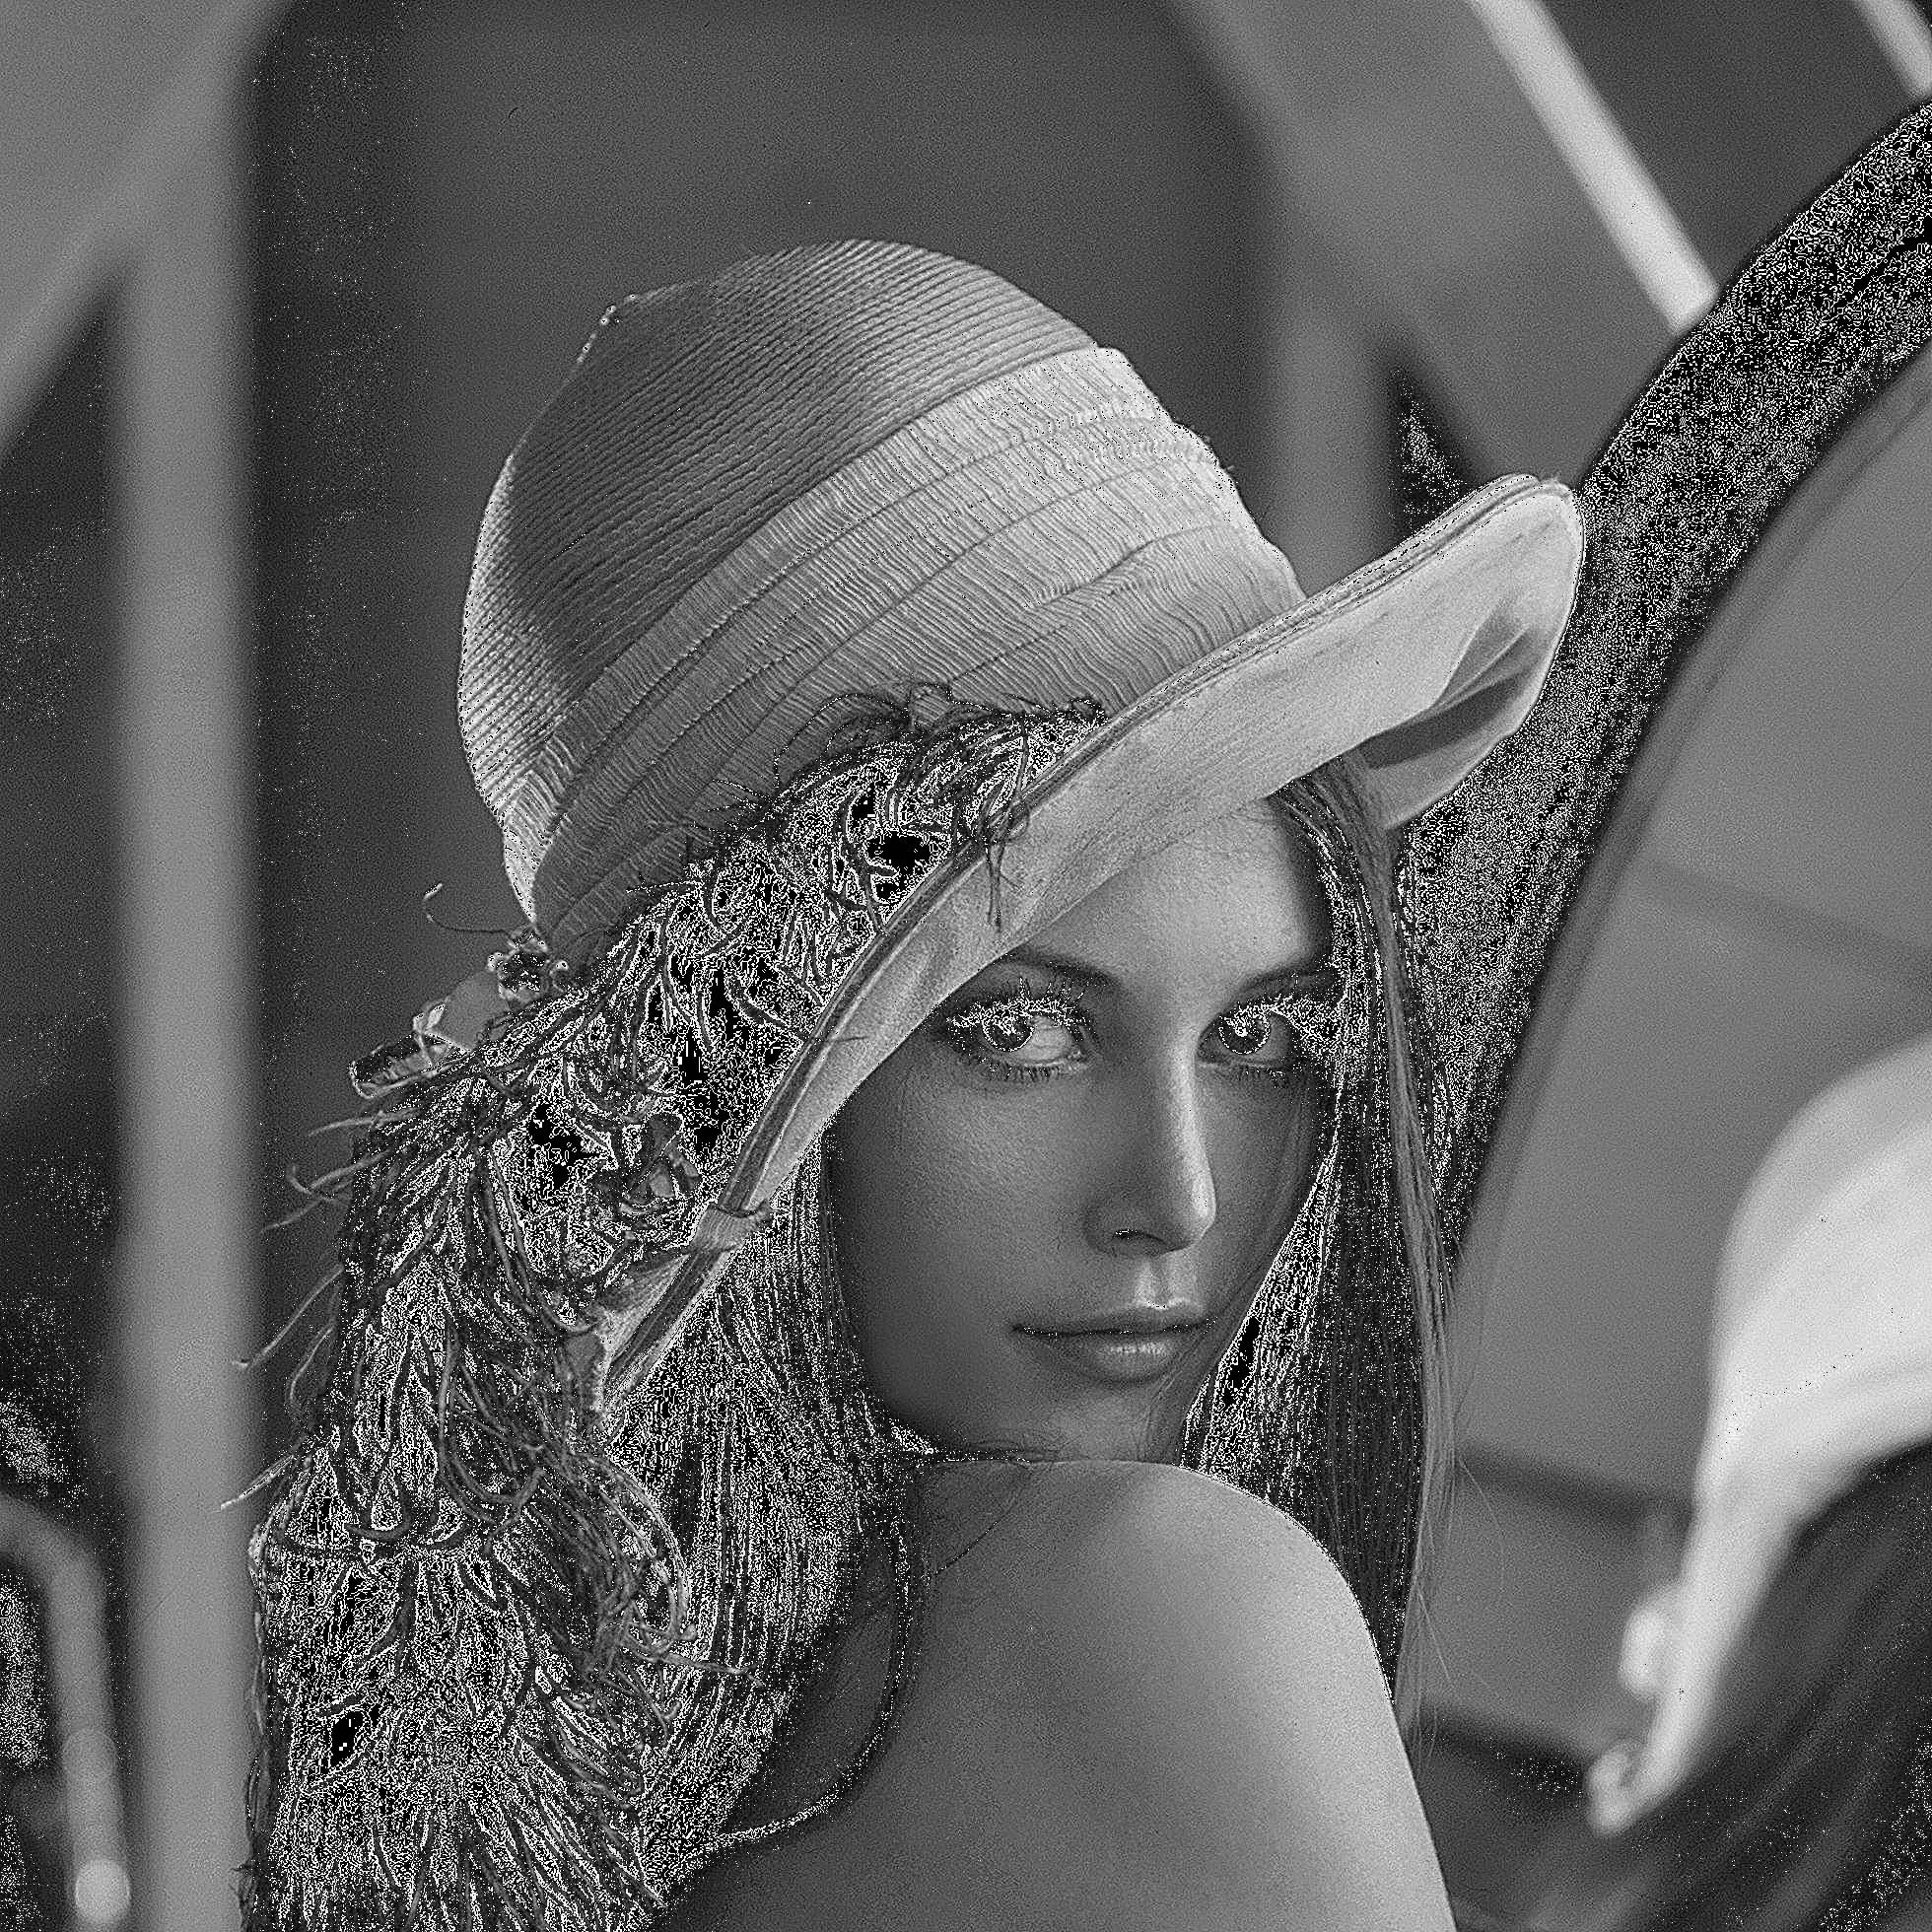
\includegraphics[width=7cm]{resources/modified/lena/lena_sharpen_5x5.jpg}
\linebreak
\tiny{Wynik działania filtru 5x5}
\end{center}

\begin{center}
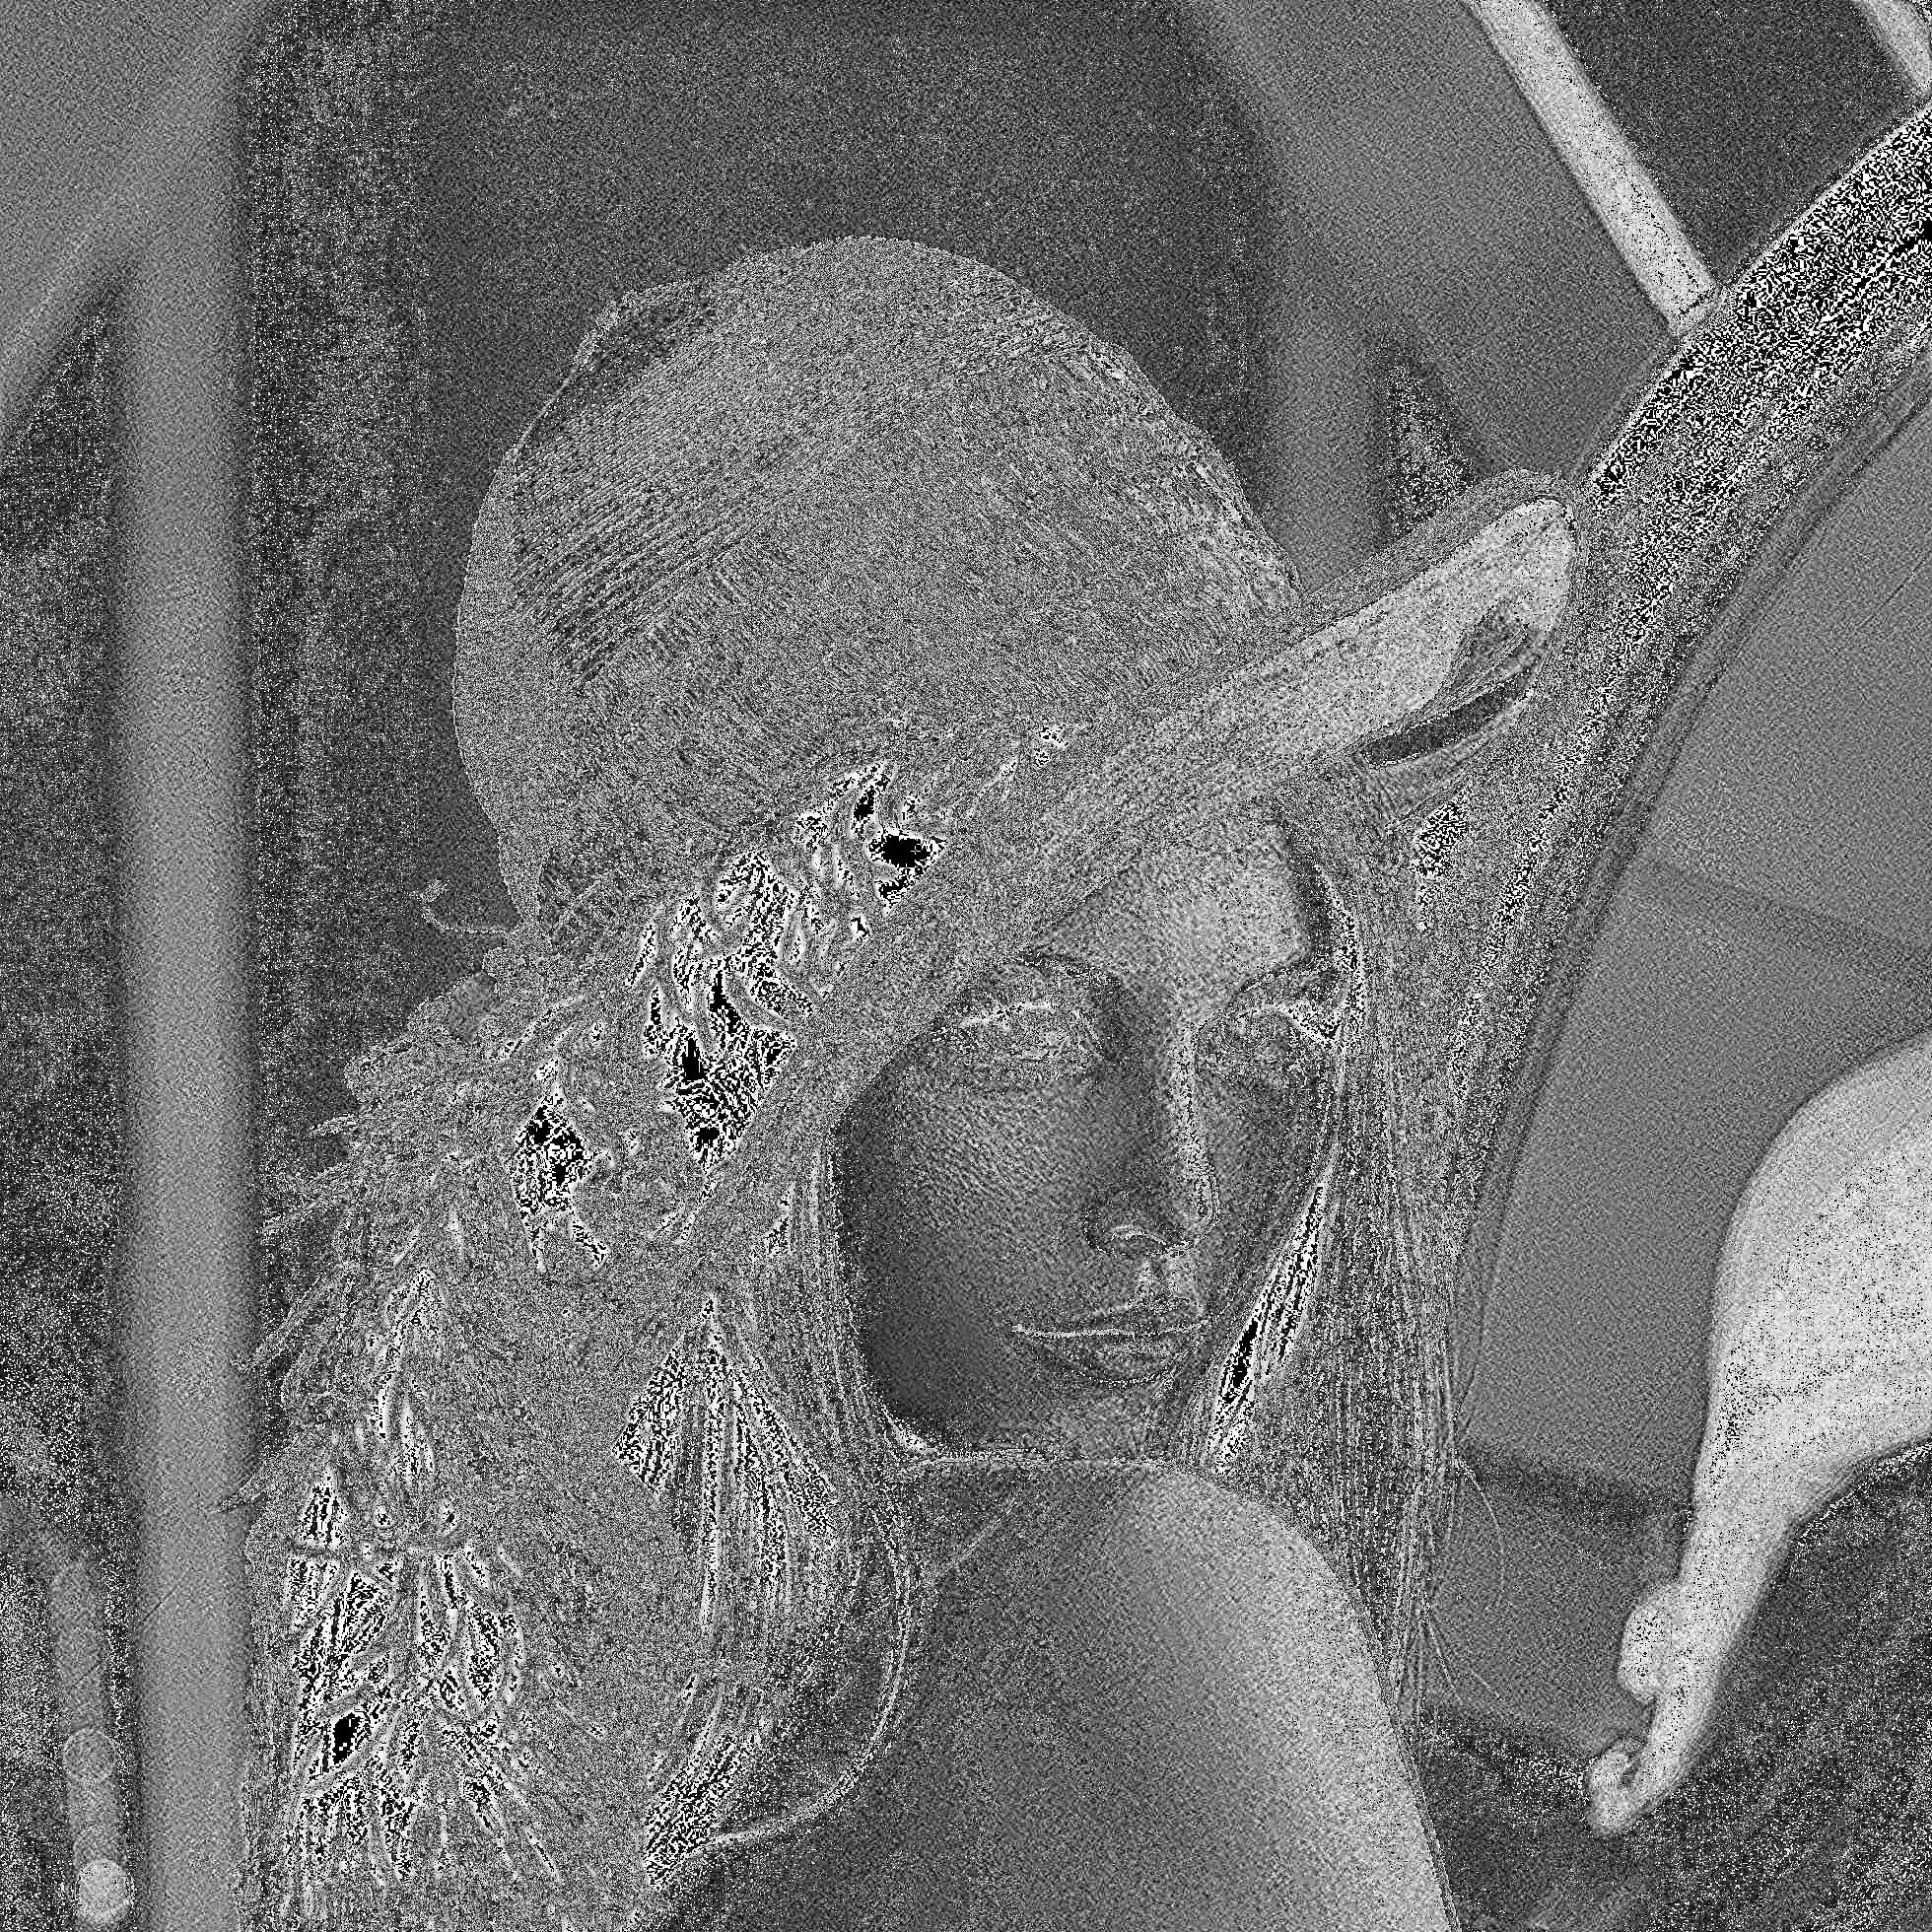
\includegraphics[width=7cm]{resources/modified/lena/lena_sharpen_11x11.jpg}
\linebreak
\tiny{Wynik działania filtru 11x11}
\end{center}

\pagebreak
\paragraph{\indent Działanie filtrów wyostrzających powoduje powstanie dodatkowych punktów kontrastu tym silniejszych im większa była różnica wartości między pikselami na osi oraz pikselem środkowym. W przypadku filtrów małych filtrów (np 3x3 i 5x5) podkreślone zostają mniej widoczne krawędzie na obrazie (np w piórach w kapeluszu). Zastosowanie większych filtrów powoduje powstanie dużego szumu na całym obrazie oraz znacznych zniekształceń w miejscach wyraźnym krawędzi. Poniżej przykłady na prostszym obrazie :}

\begin{center}
\text{wyniki działania filtrów 3x3 oraz 7x7:}\\
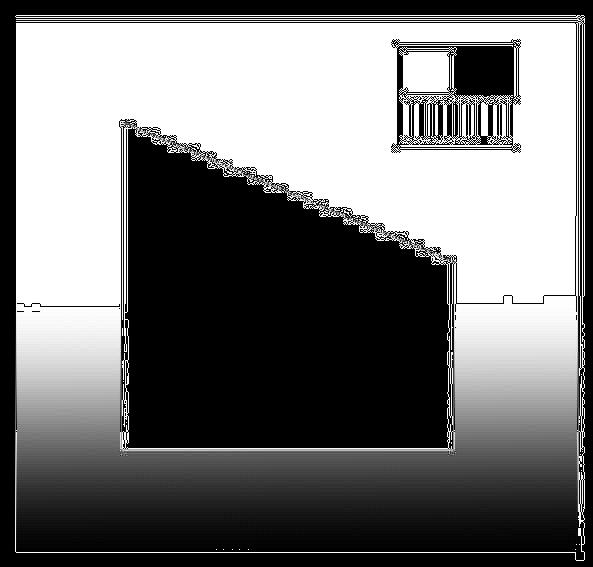
\includegraphics[width=7cm]{resources/modified/sample/sample_sharpen_3x3.jpg}
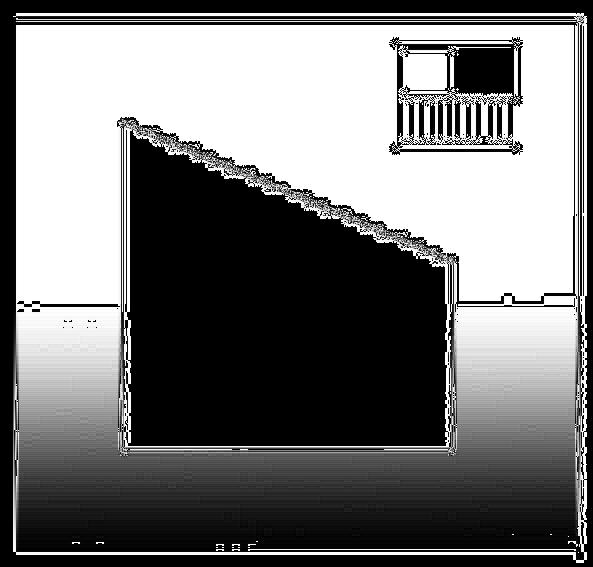
\includegraphics[width=7cm]{resources/modified/sample/sample_sharpen_7x7.jpg}
\\
\text{wyniki działania filtrów 11x11 oraz 21x21:}\\
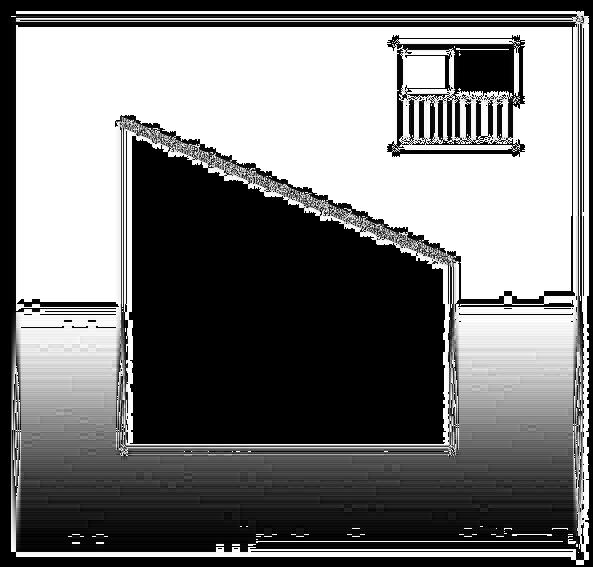
\includegraphics[width=7cm]{resources/modified/sample/sample_sharpen_11x11.jpg}
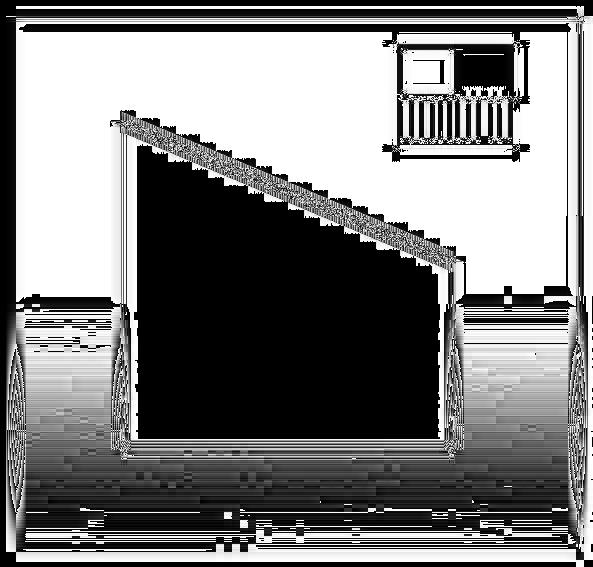
\includegraphics[width=7cm]{resources/modified/sample/sample_sharpen_21x21.jpg}
\end{center}

\pagebreak
\subsection{Dodatkowe filtry}

\begin{center}
\text{wyniki działania filtrów 3x11 oraz 11x3:}\\
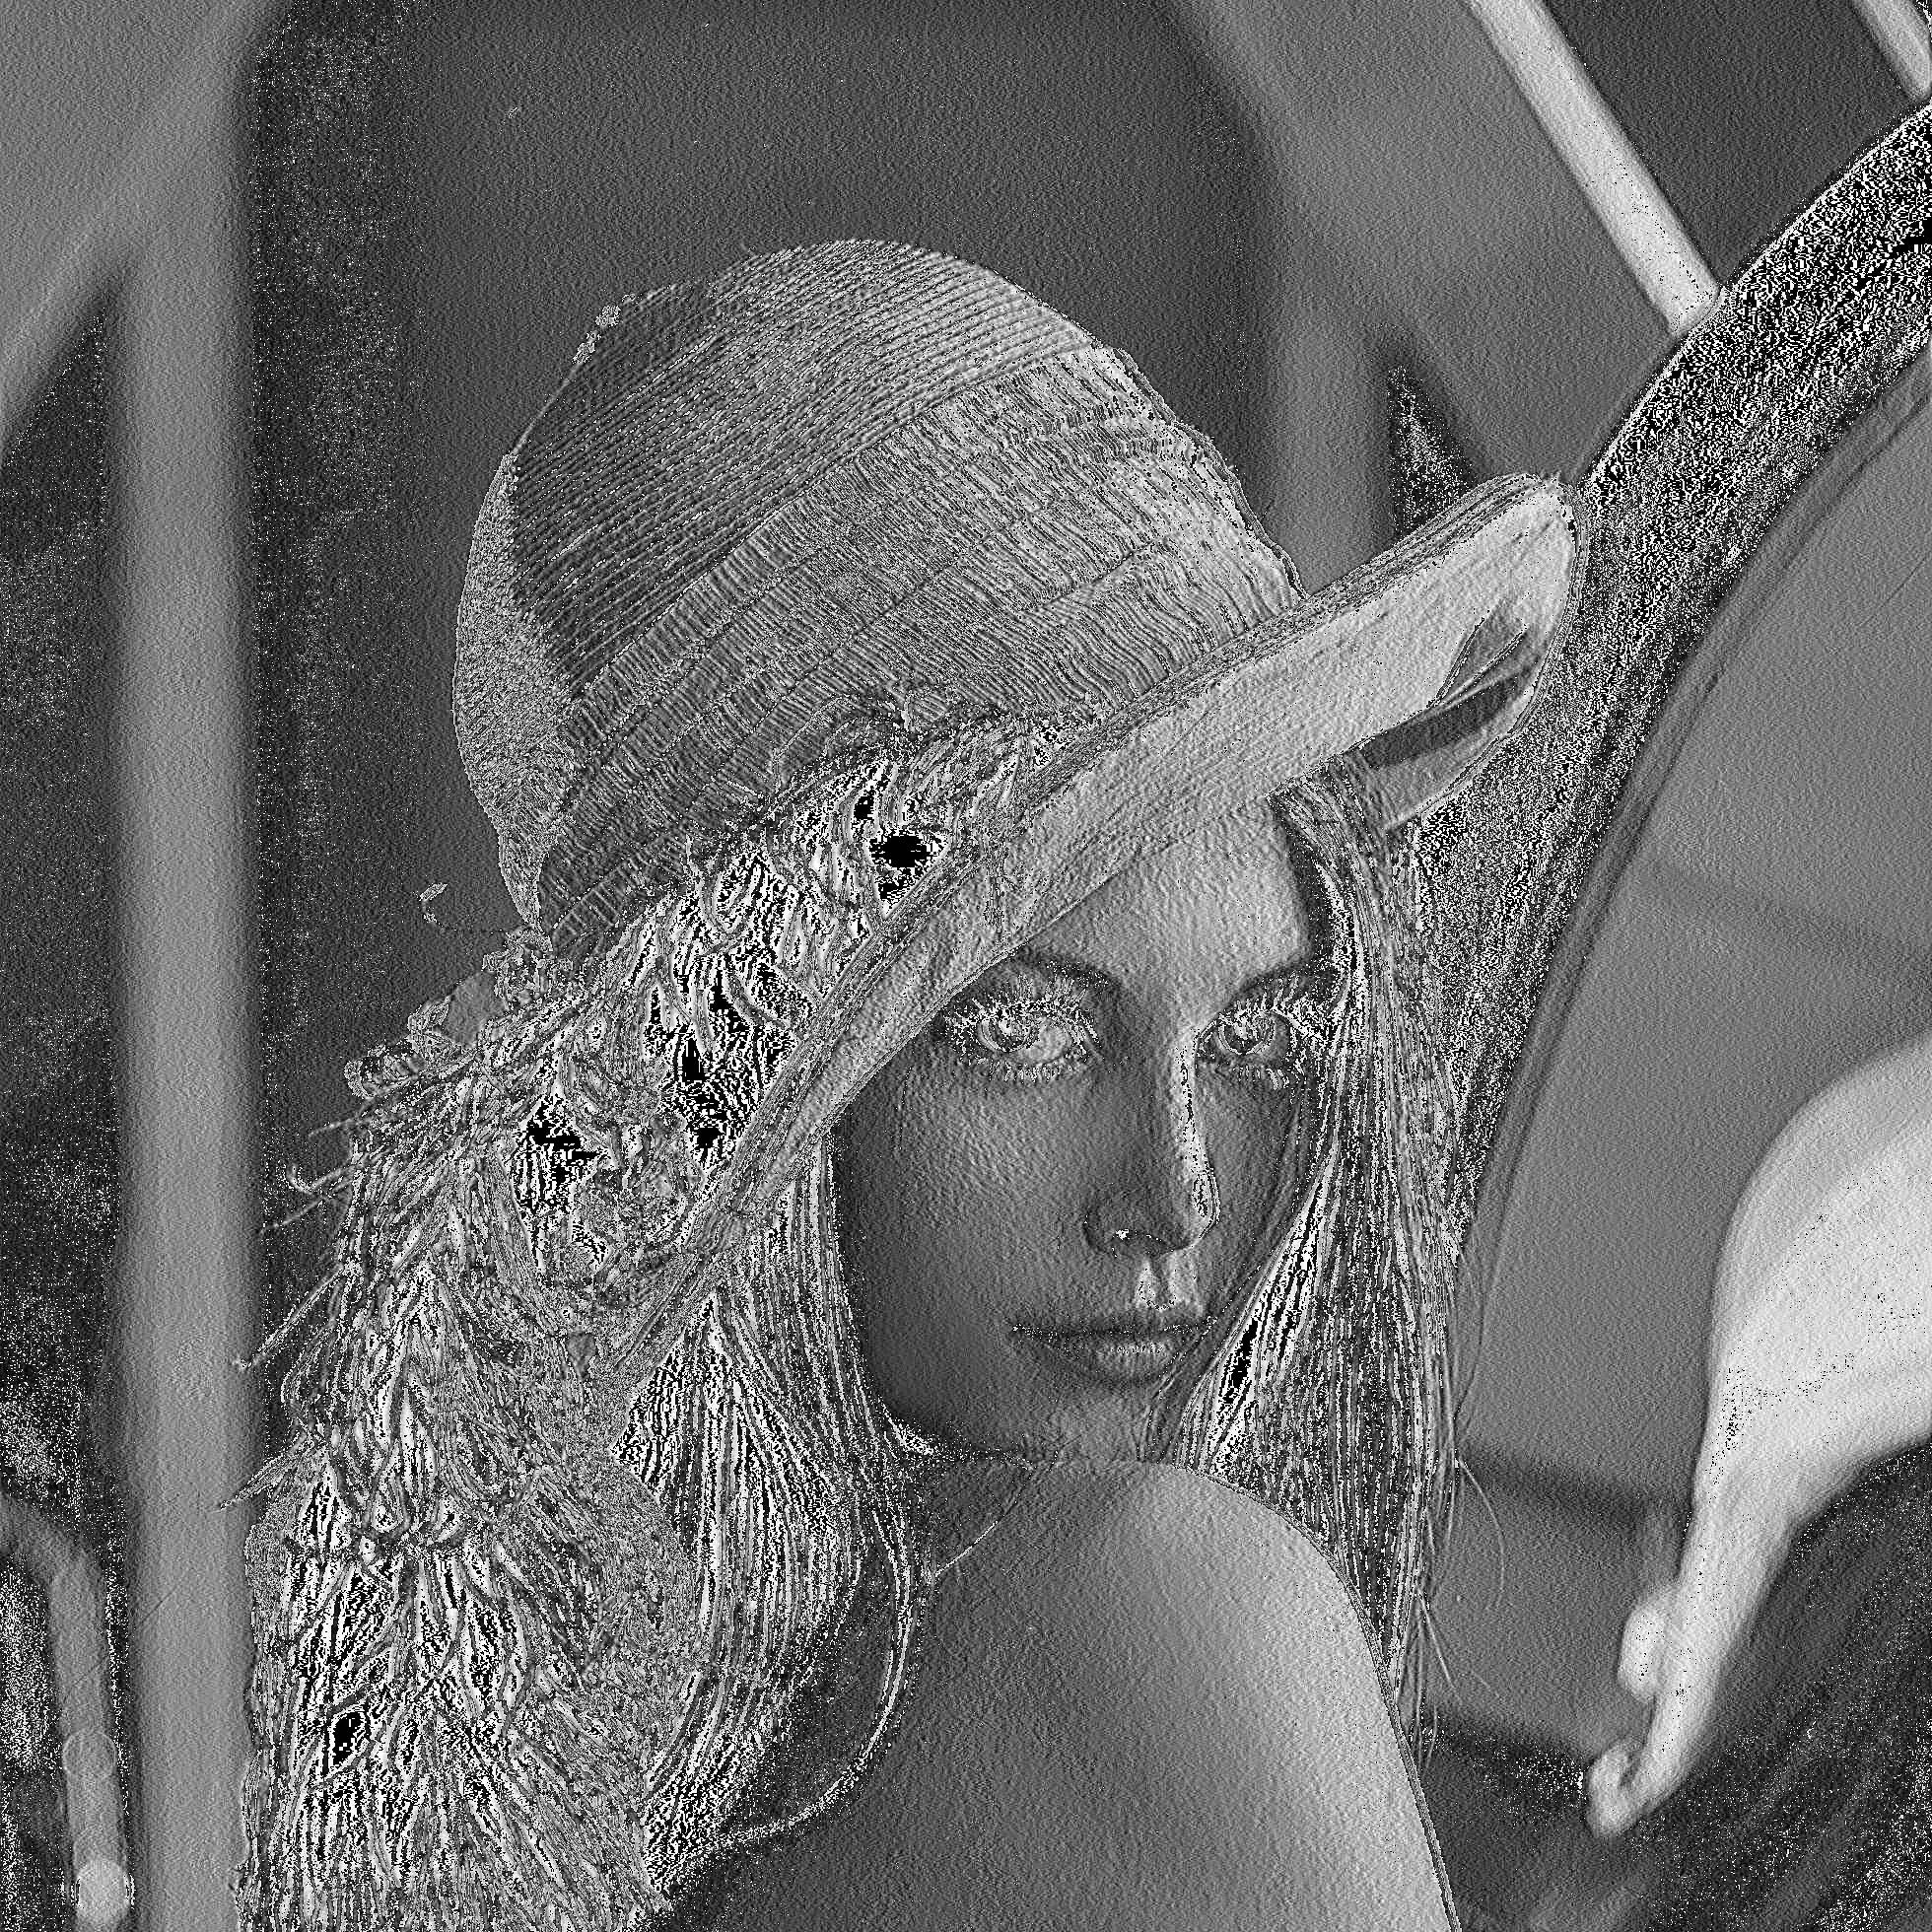
\includegraphics[width=7cm]{resources/modified/lena/lena_sharpen_3x11.jpg}
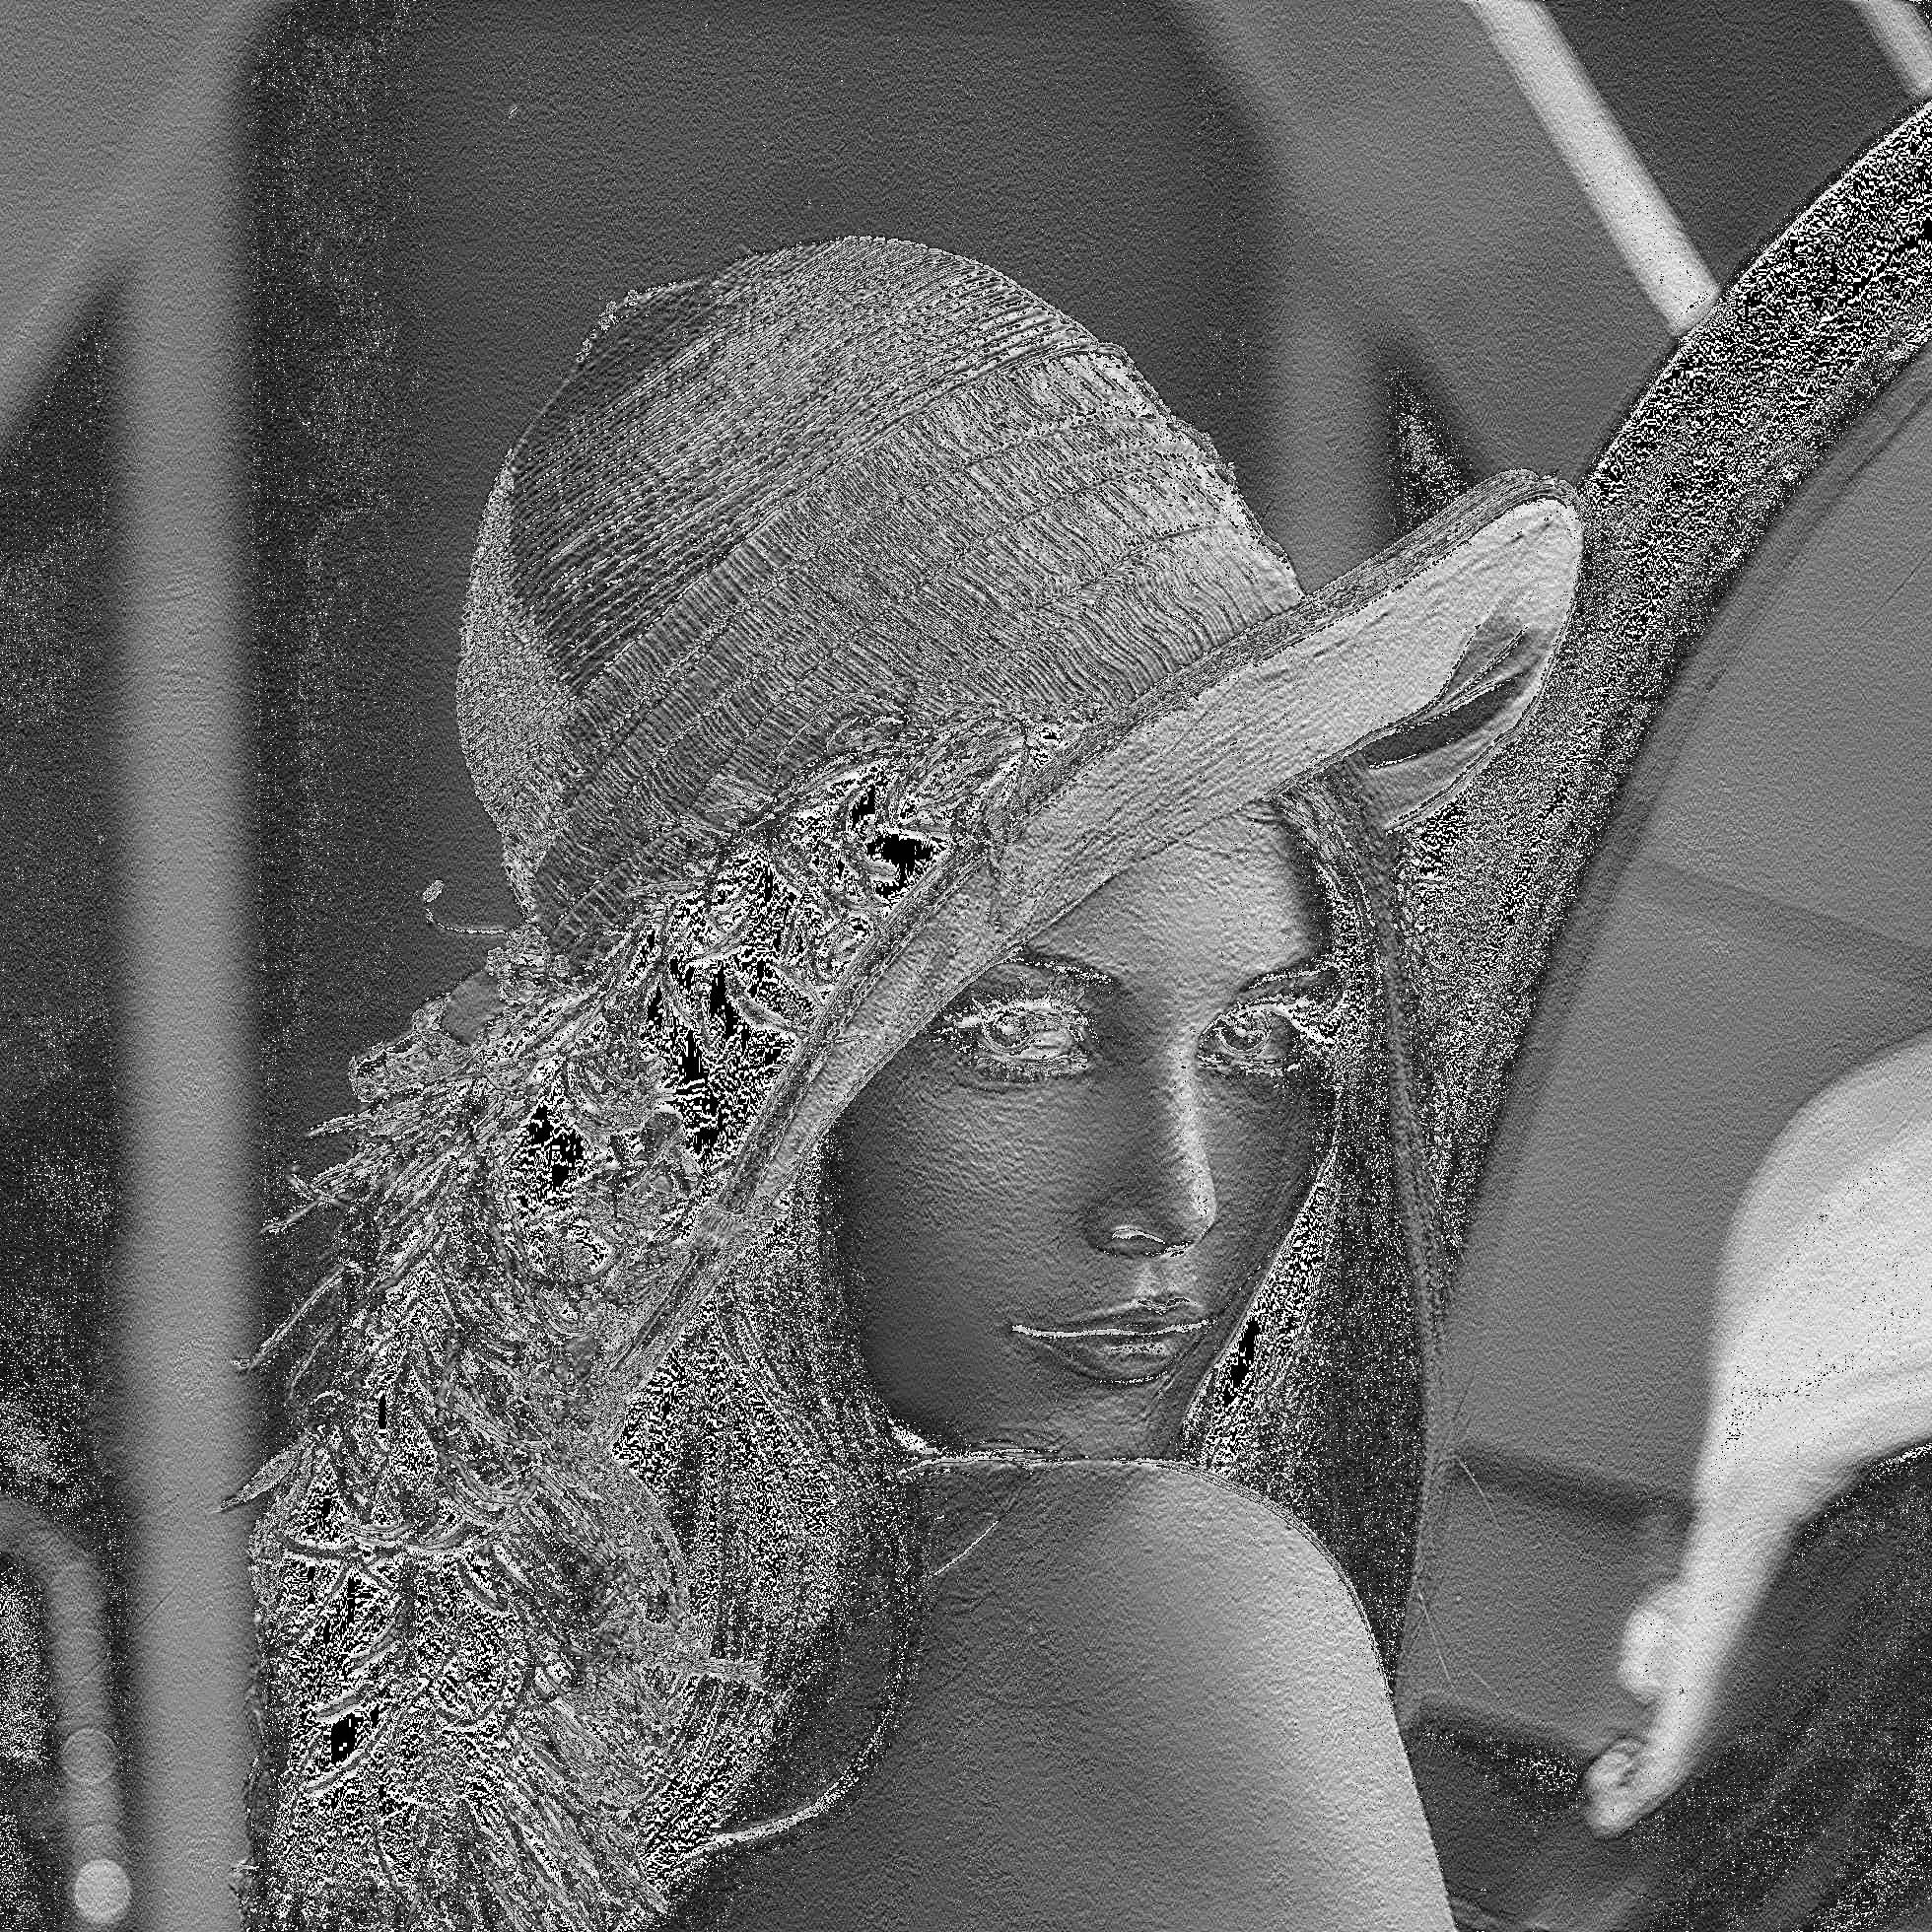
\includegraphics[width=7cm]{resources/modified/lena/lena_sharpen_11x3.jpg}
\\
\text{wyniki działania filtrów 7x7 oraz 9x9:}\\
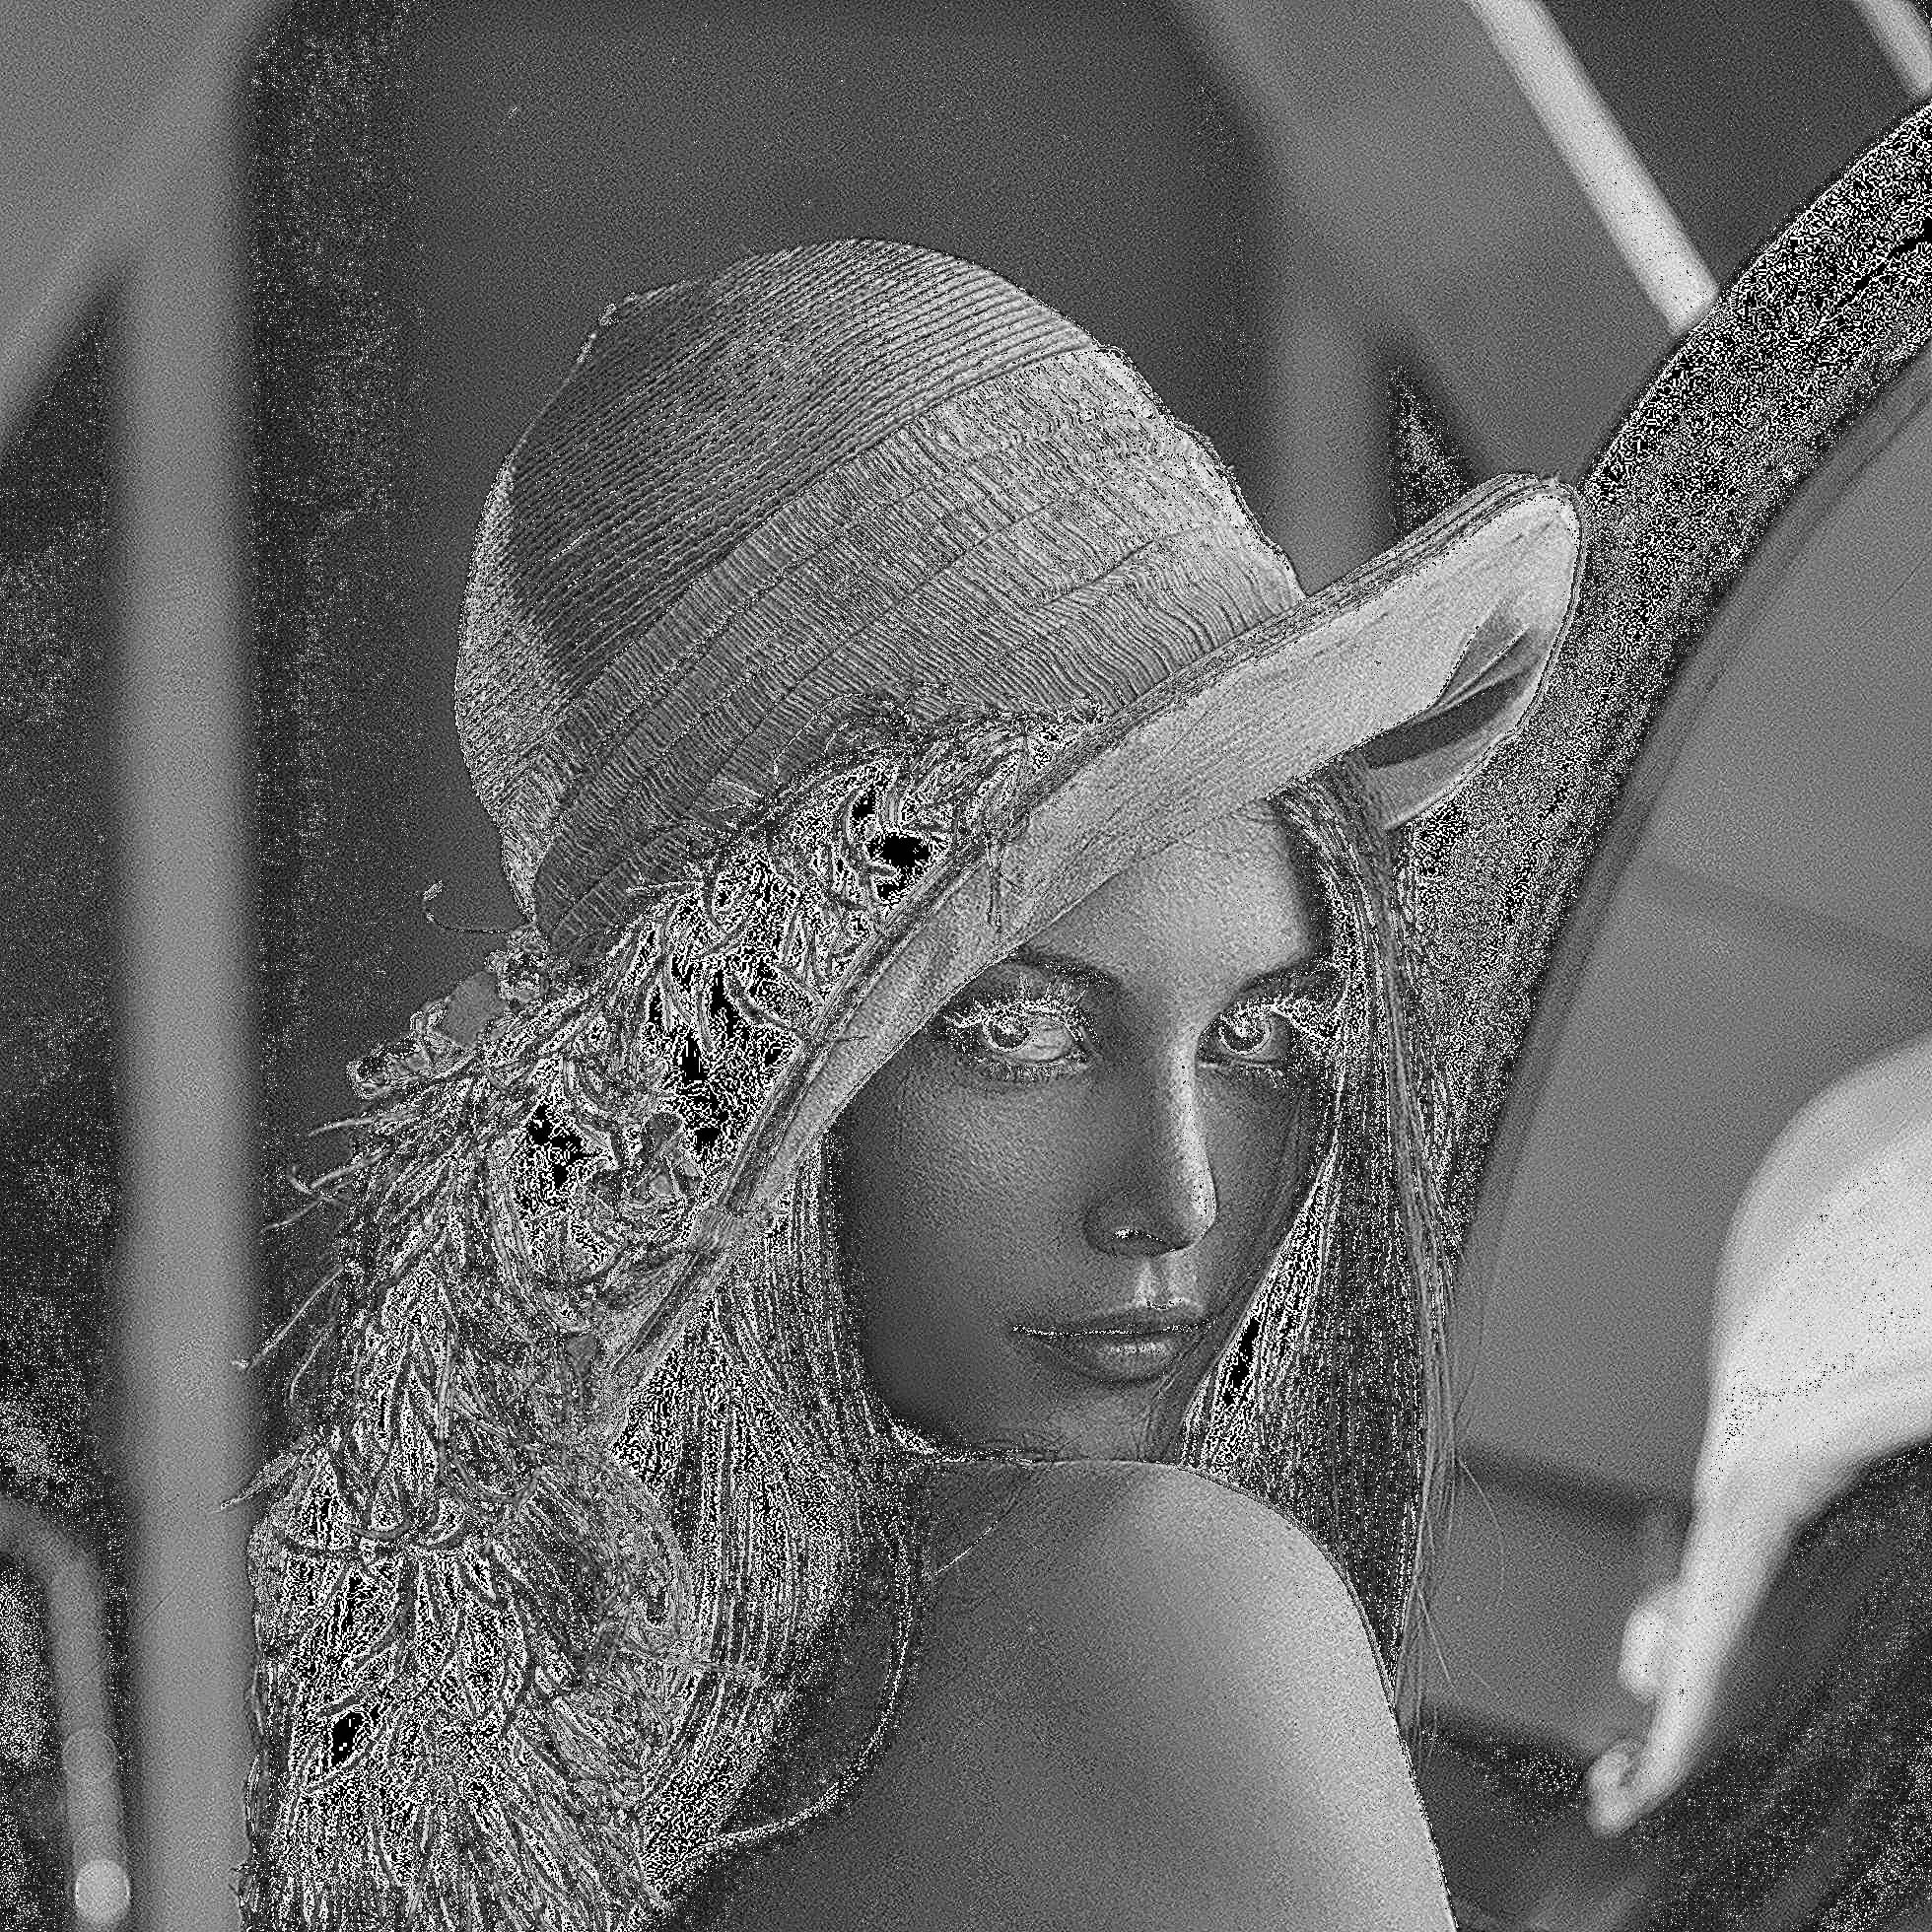
\includegraphics[width=7cm]{resources/modified/lena/lena_sharpen_7x7.jpg}
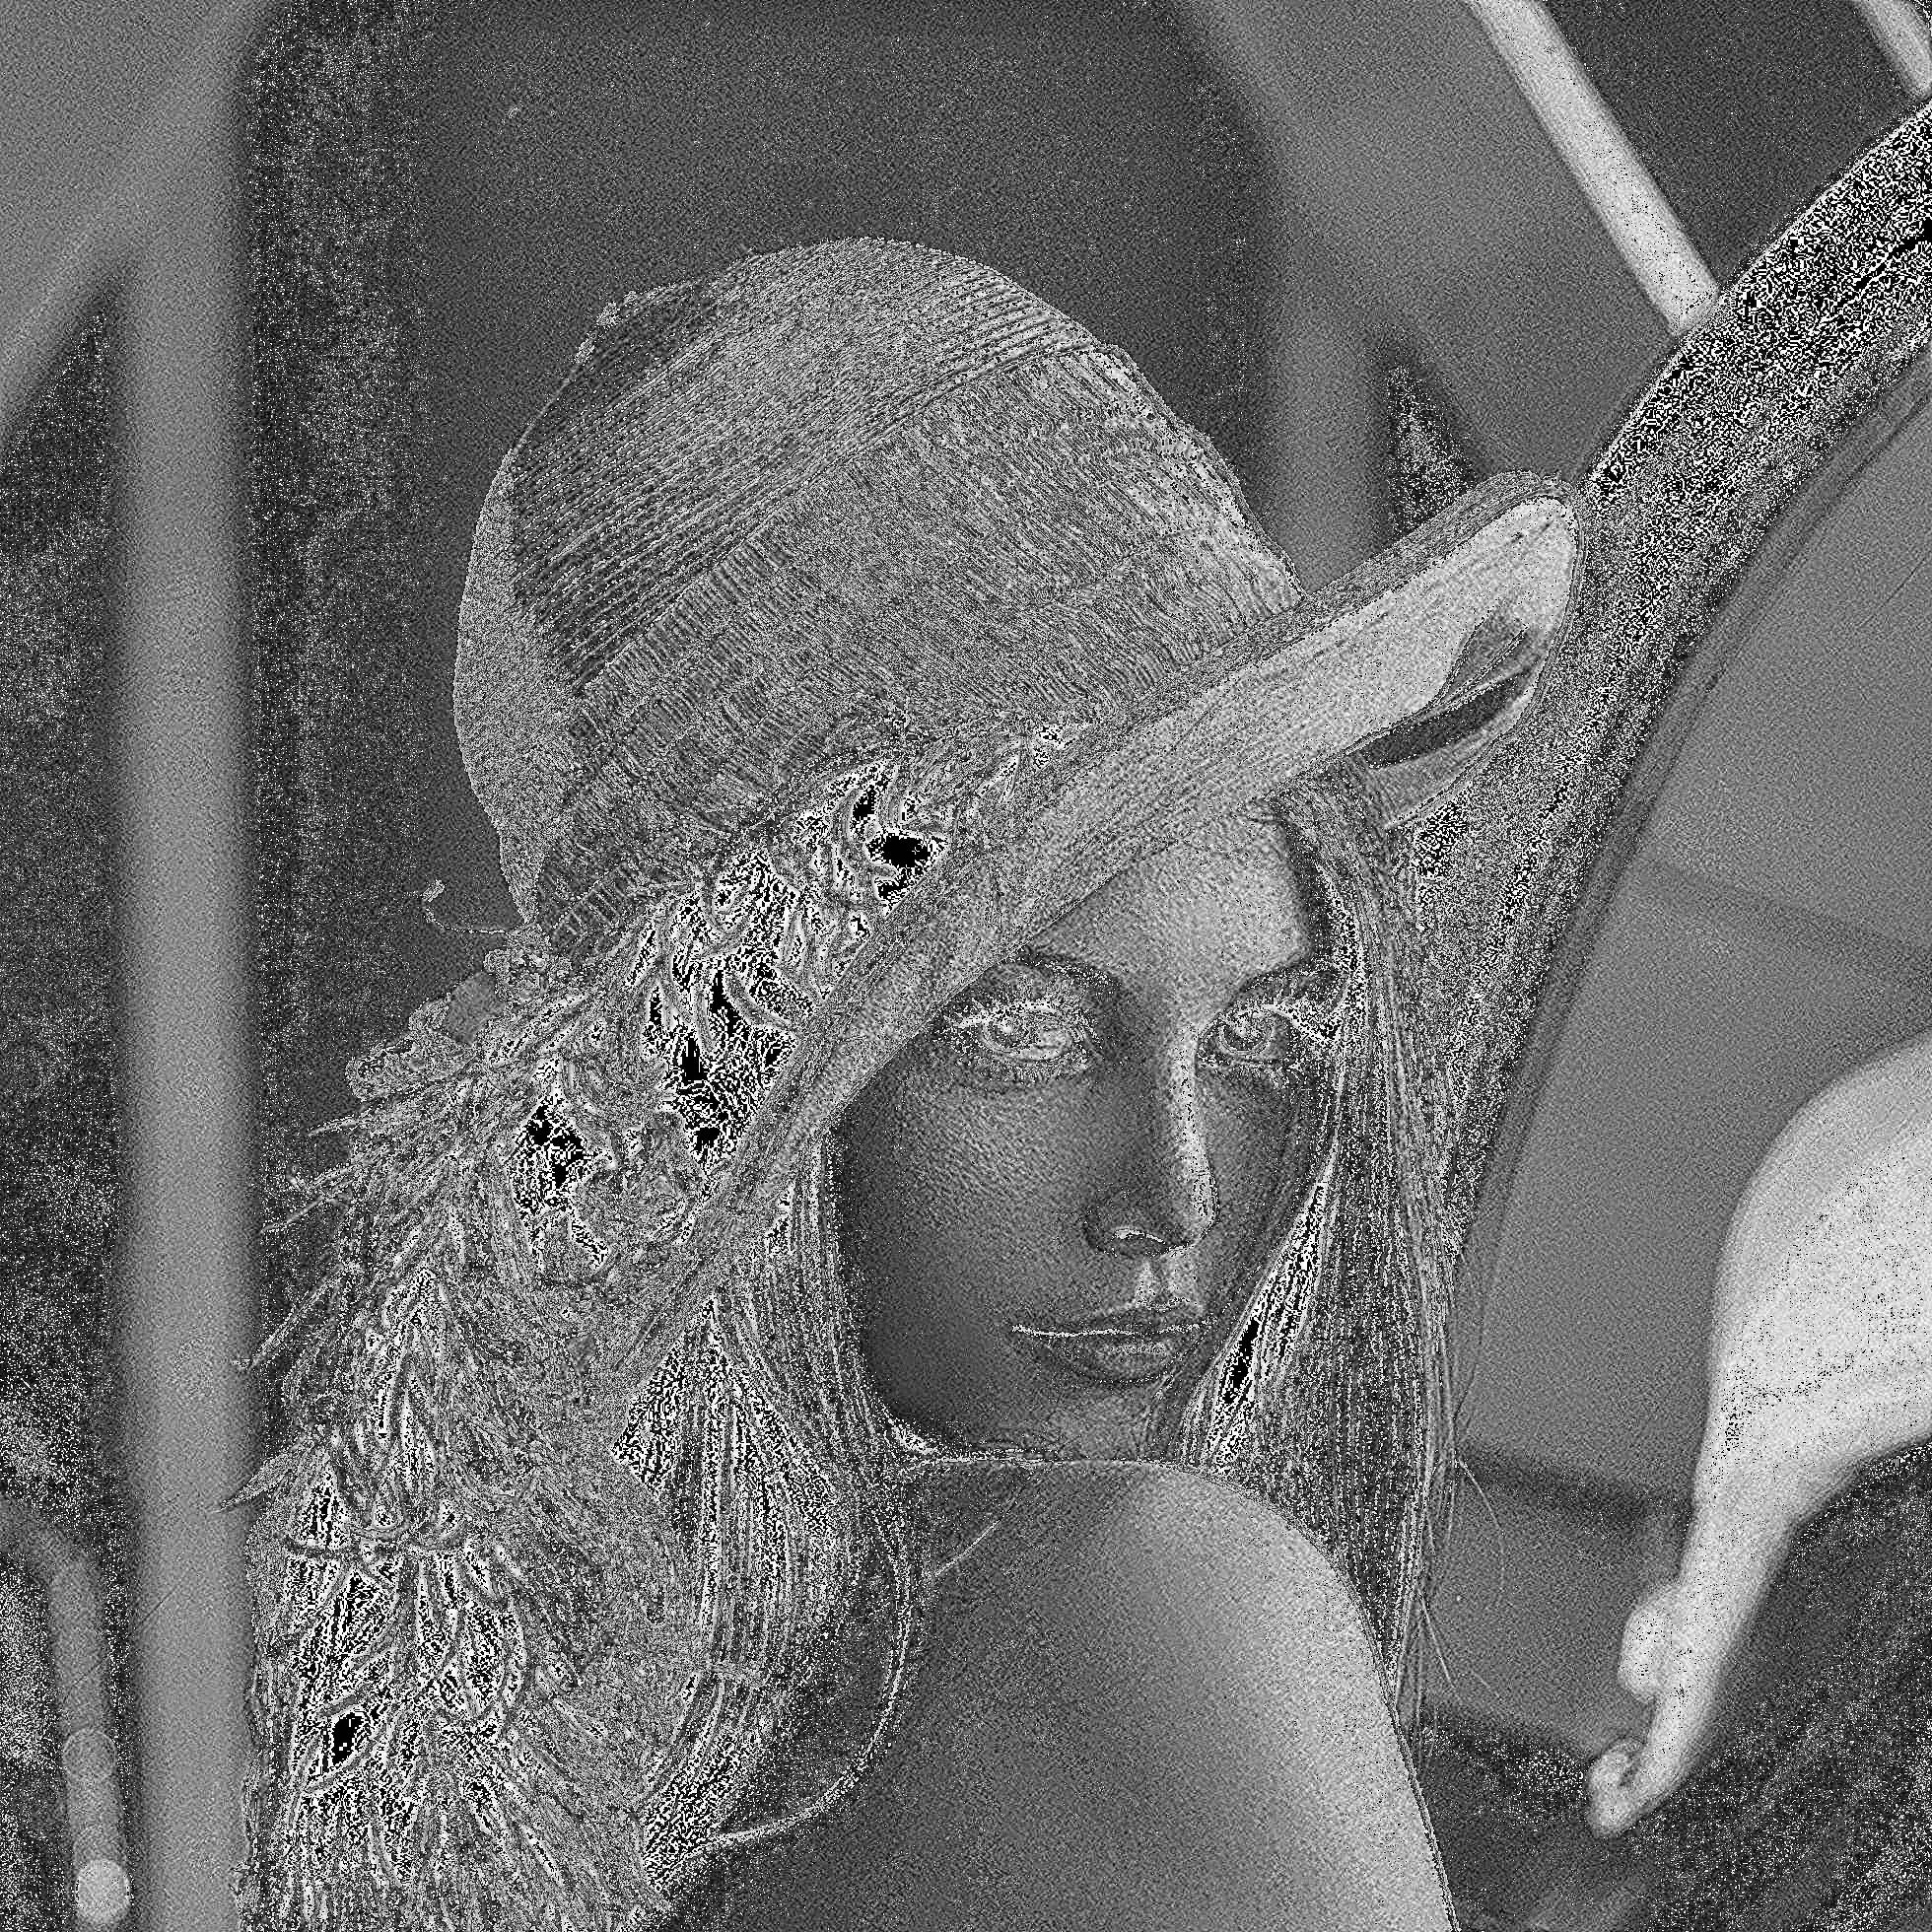
\includegraphics[width=7cm]{resources/modified/lena/lena_sharpen_9x9.jpg}
\\
\text{wyniki działania filtrów 11x11 oraz 21x21:}\\
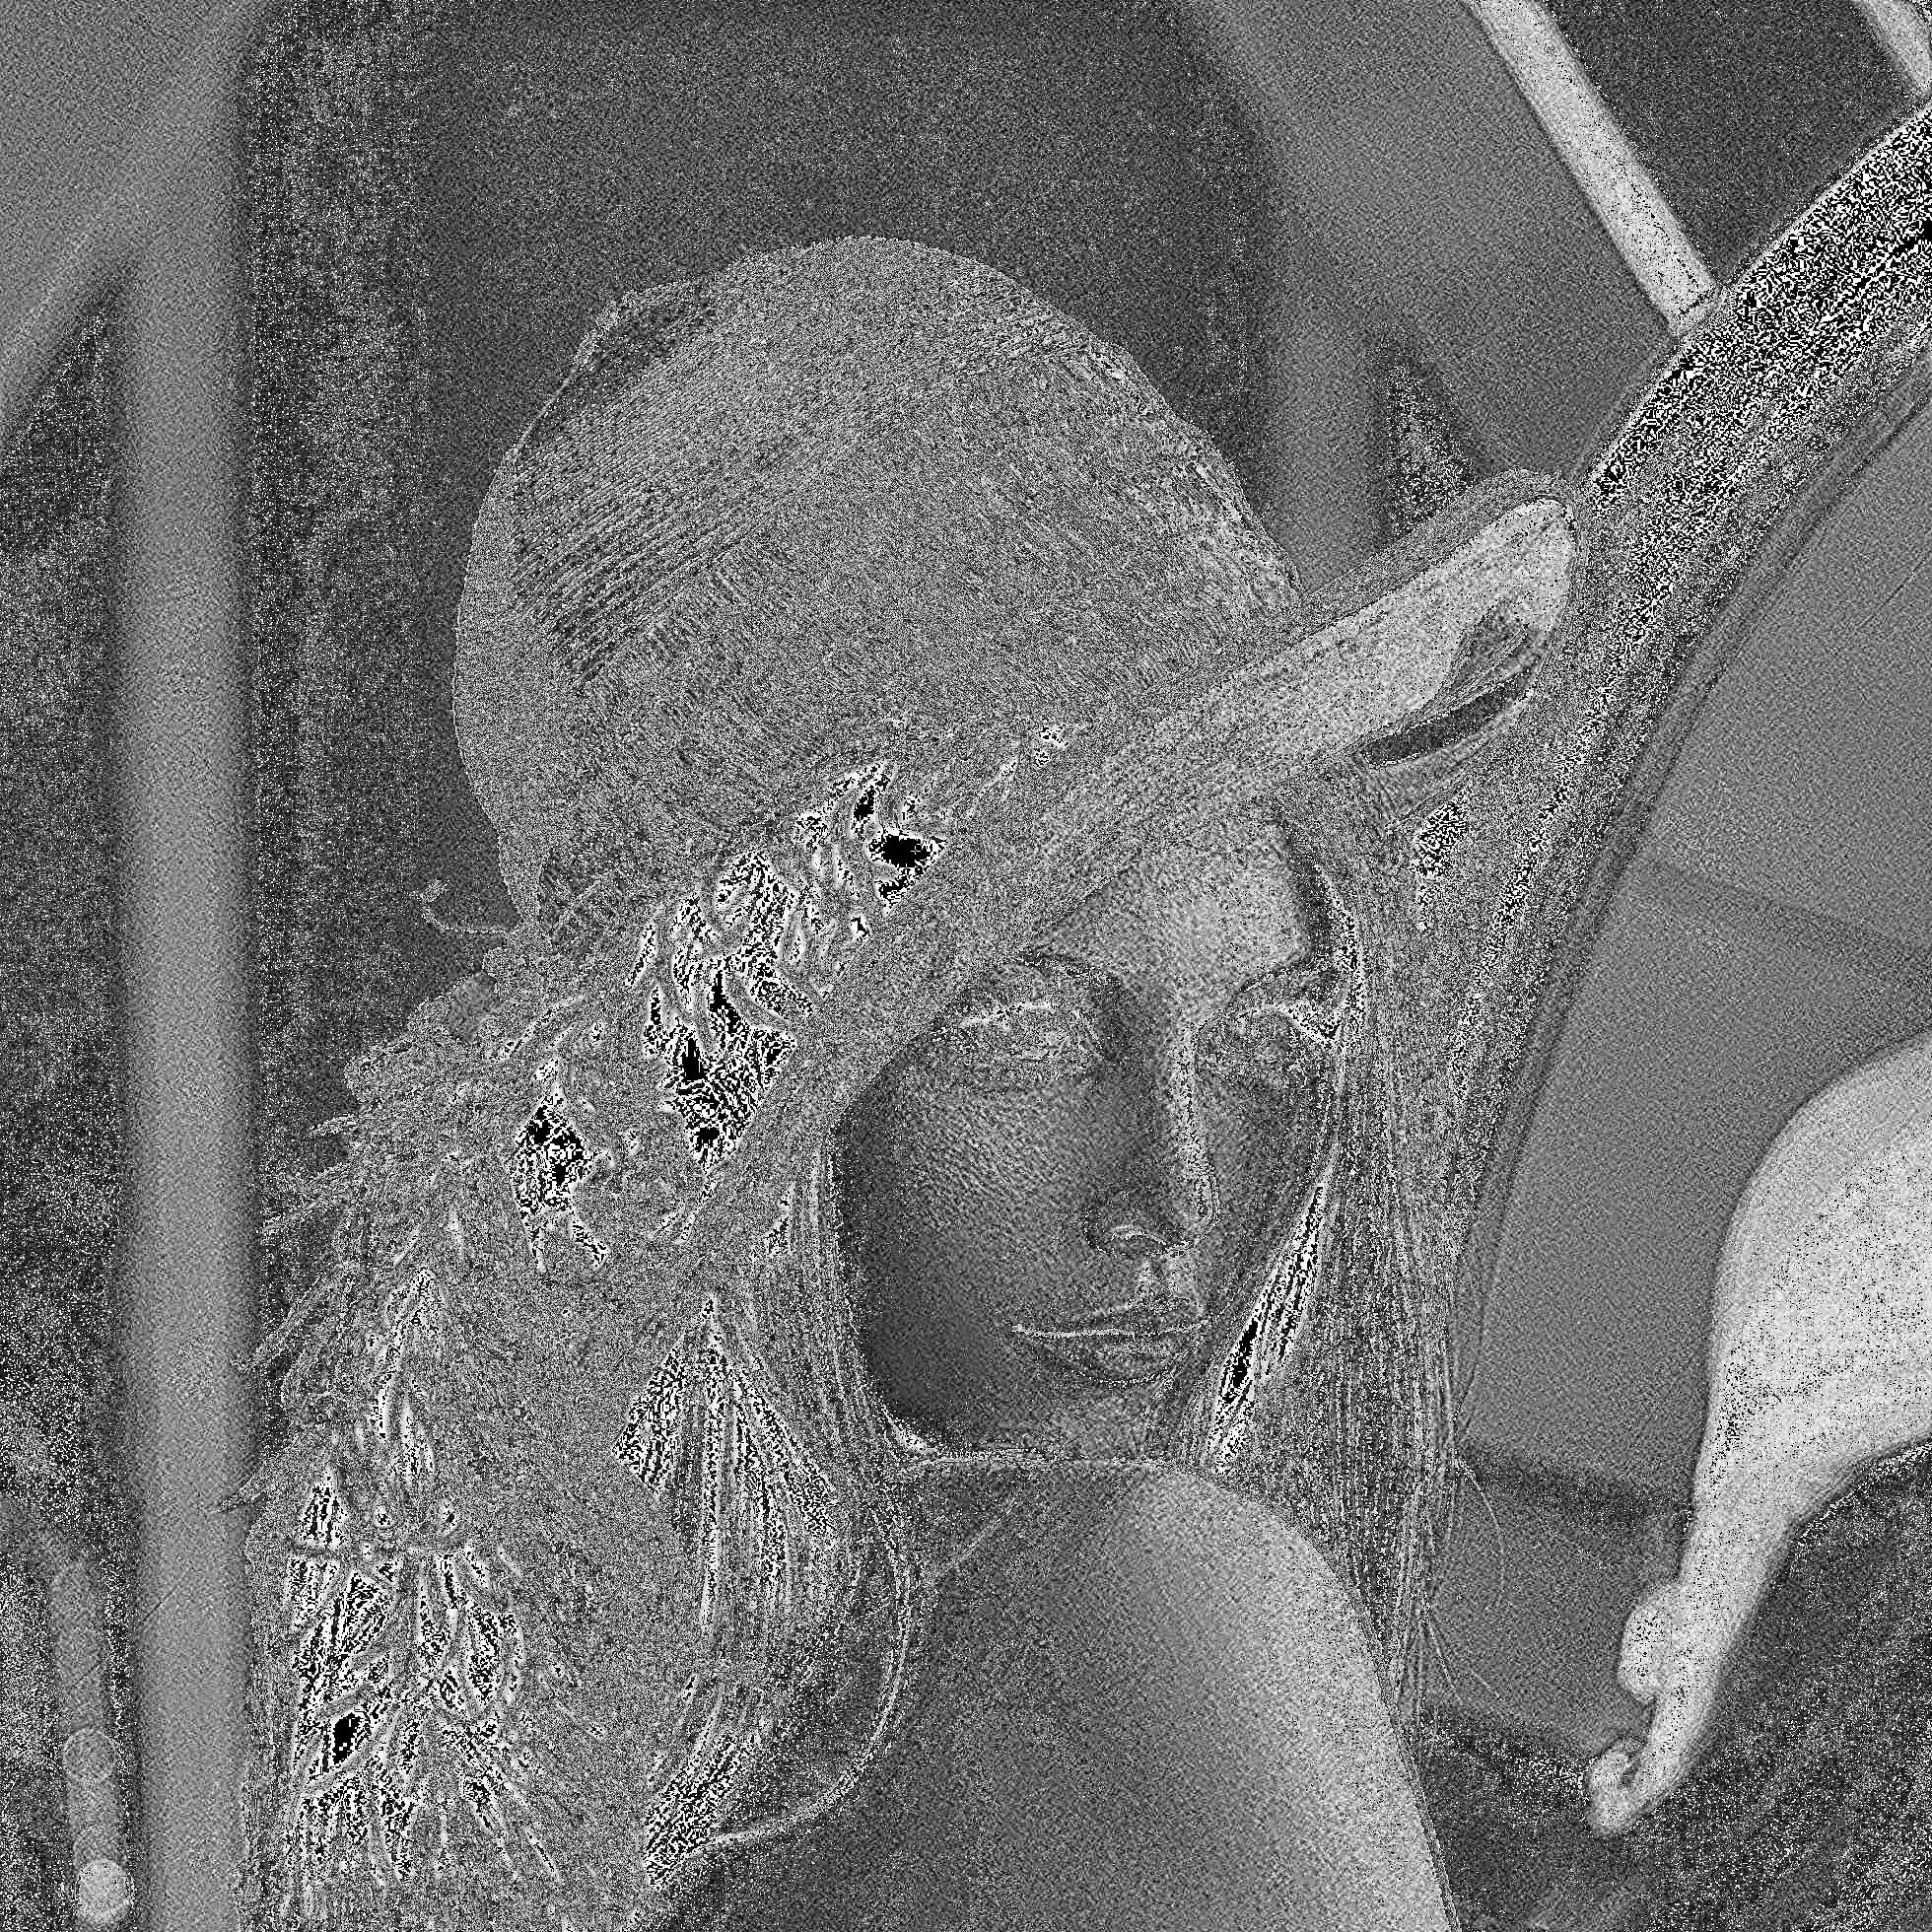
\includegraphics[width=7cm]{resources/modified/lena/lena_sharpen_11x11.jpg}
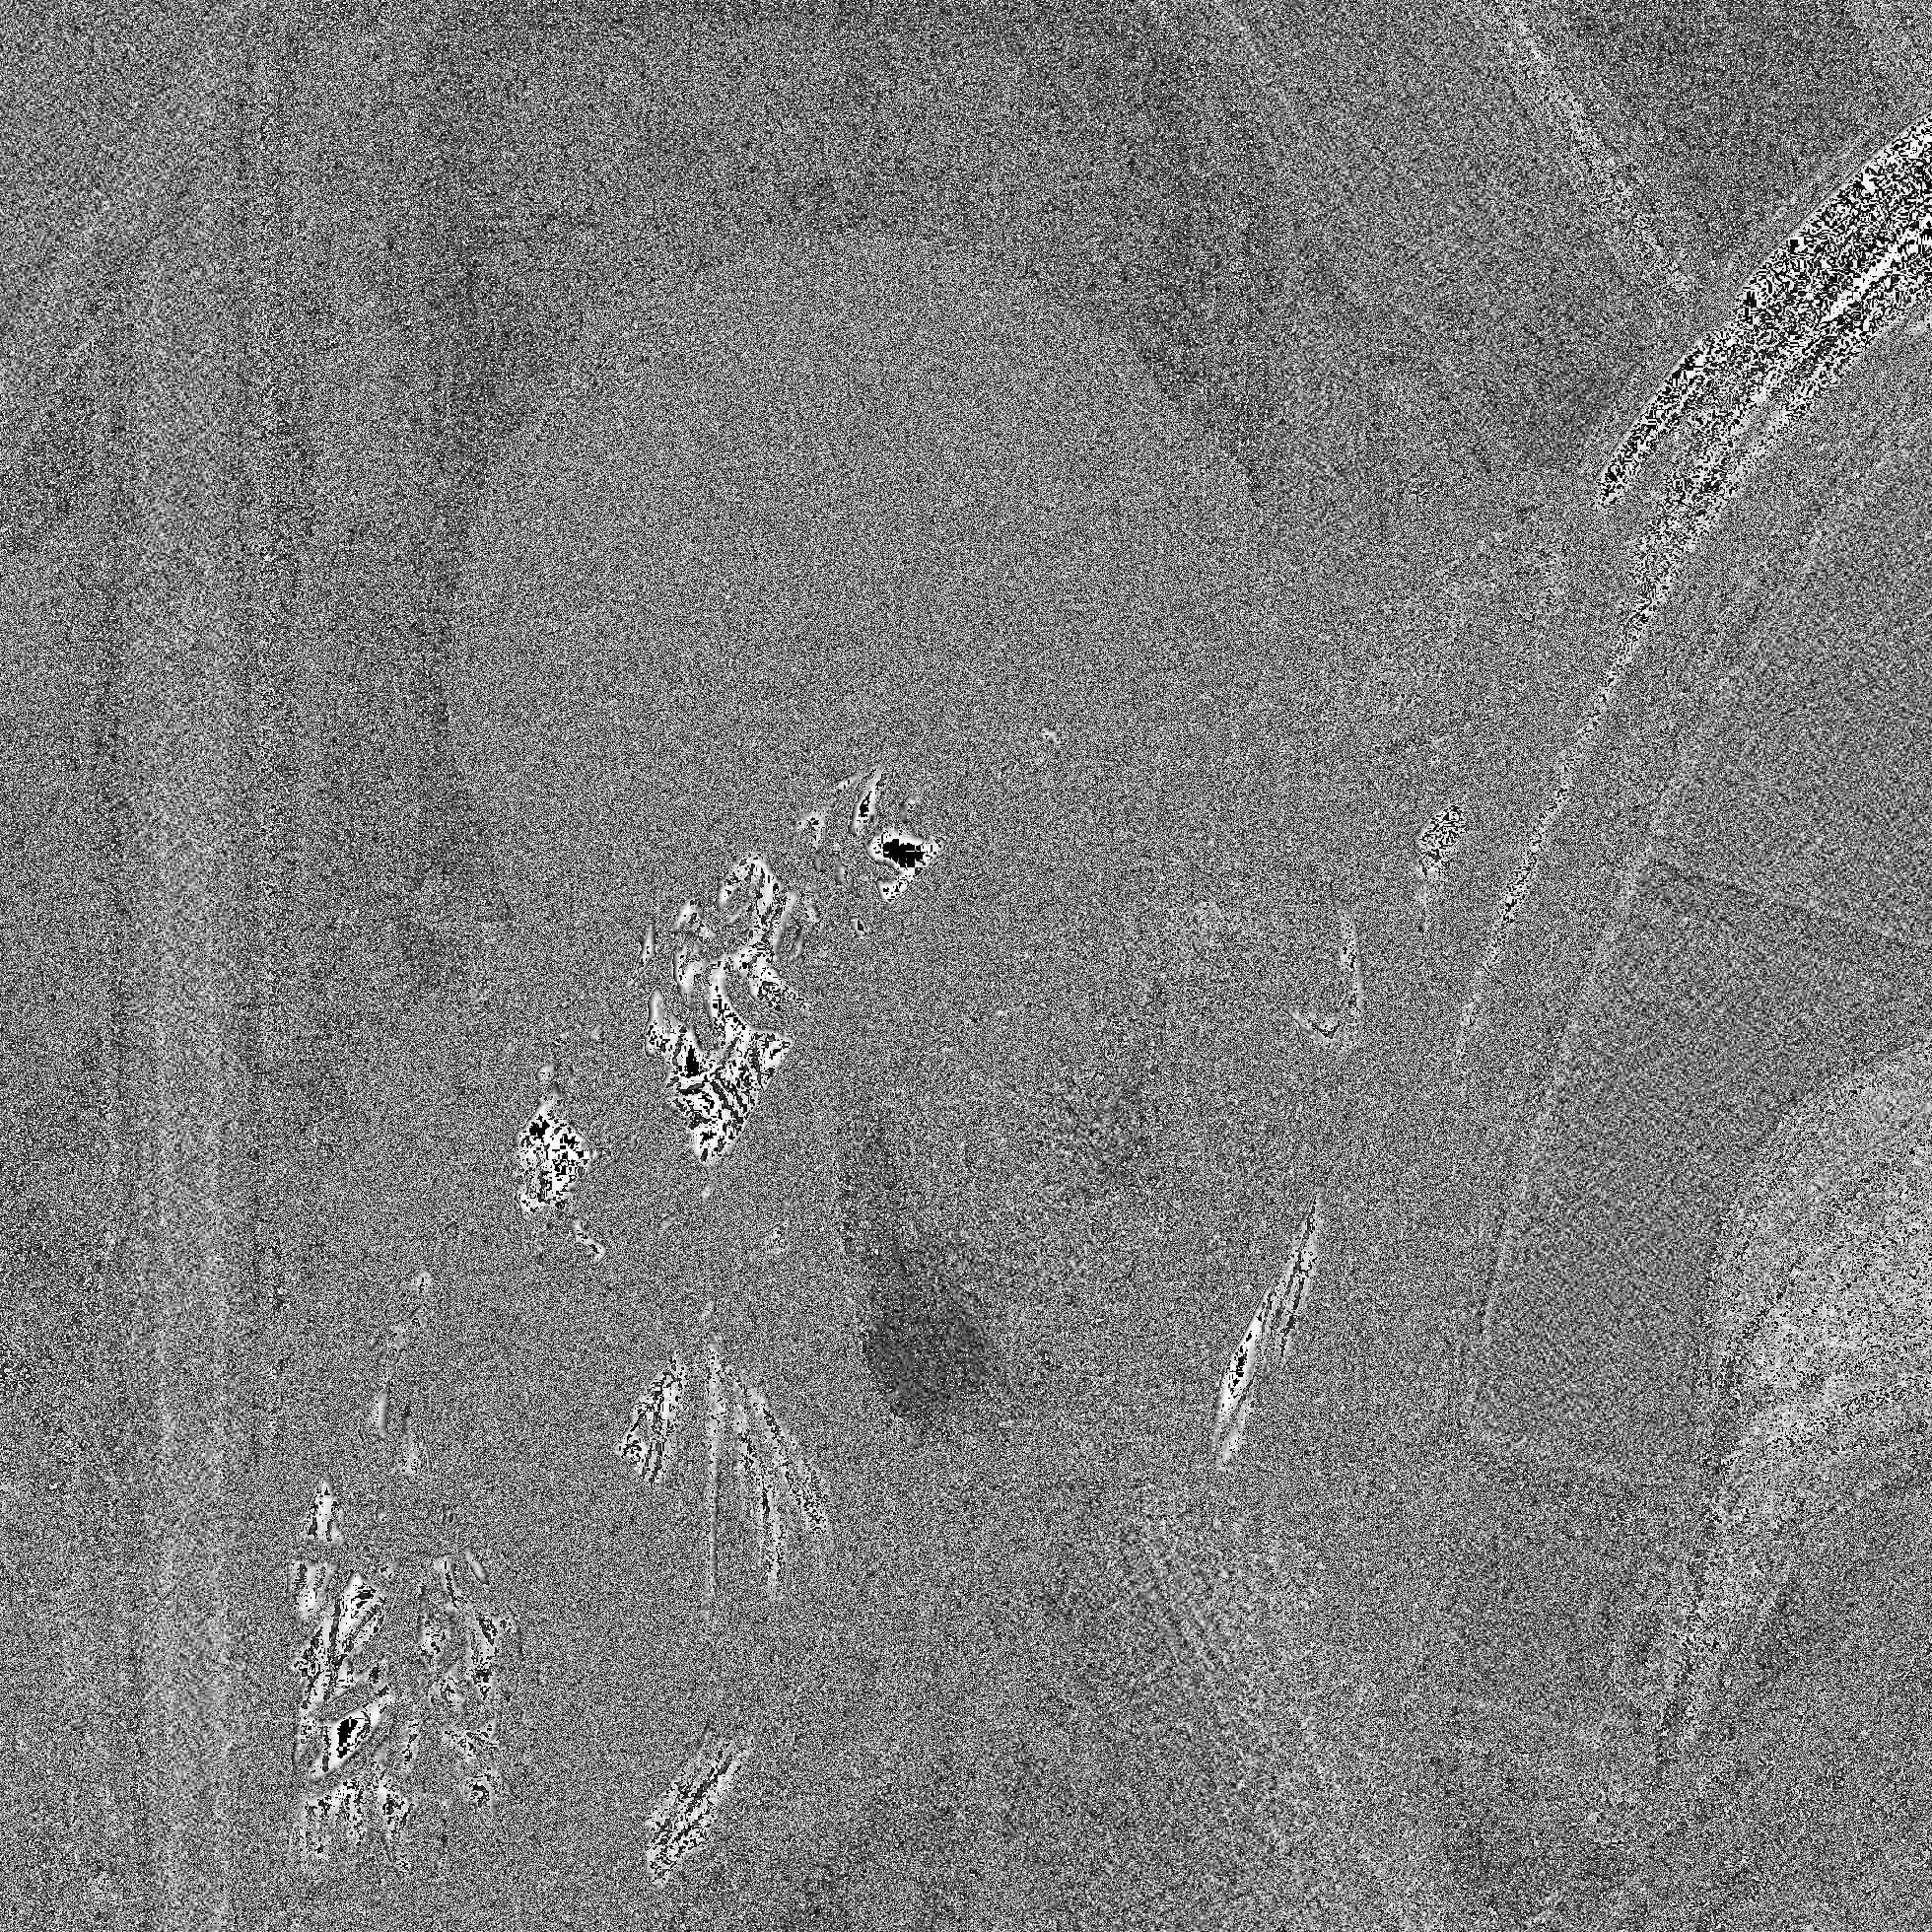
\includegraphics[width=7cm]{resources/modified/lena/lena_sharpen_21x21.jpg}
\end{center}

\pagebreak
\paragraph{\indent W przeciwieństwie do filtrów uśredniających, filtry wyostrzające nie zmieniają tak mocno skutków działania w zależności od stosunku szerokości do wysokości. Poniżej przykłady na prostszym obrazie :}

\begin{center}
\text{wyniki działania filtrów 40x1 oraz 1x40:}\\
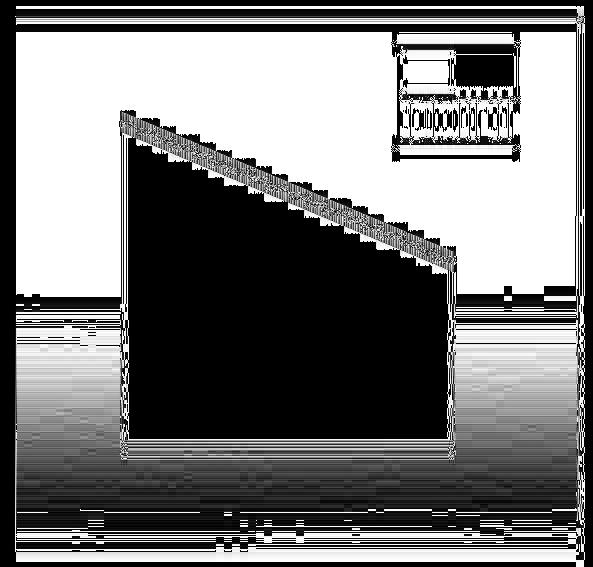
\includegraphics[width=7cm]{resources/modified/sample/sample_sharpen_21x3.jpg}
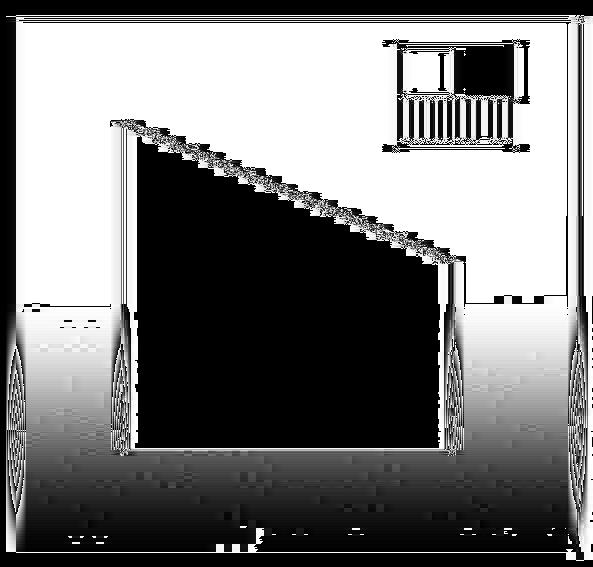
\includegraphics[width=7cm]{resources/modified/sample/sample_sharpen_3x21.jpg}
\\
\text{wyniki działania filtrów 40x5 oraz 5x40:}\\
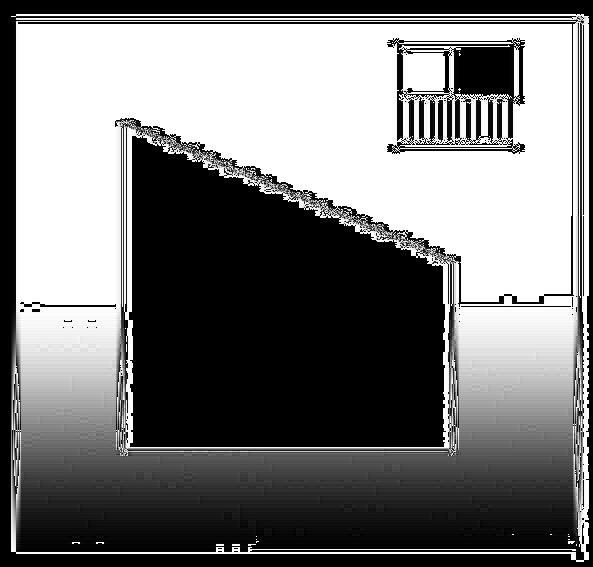
\includegraphics[width=7cm]{resources/modified/sample/sample_sharpen_5x11.jpg}
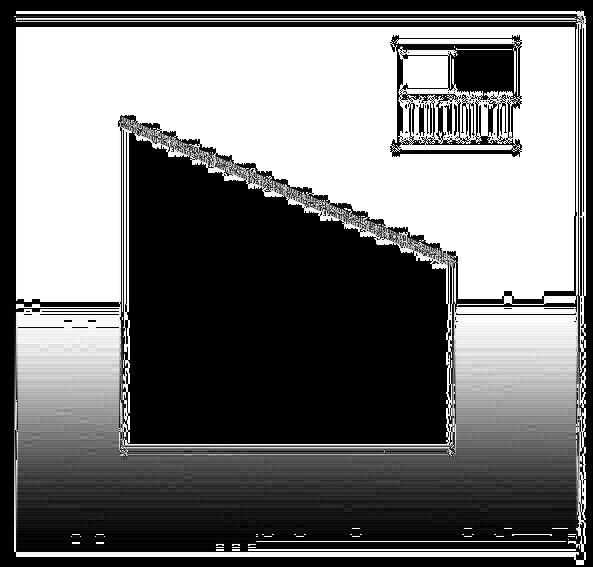
\includegraphics[width=7cm]{resources/modified/sample/sample_sharpen_11x5.jpg}
\end{center}

%%%%%%%%%%%%%%%%%%%%%%%%%%%%%%%%%%%%%%%%%%%%%%%%%%%%%%%%%%%%%%%%%%%%%%%%%%%%%%%%%%%%%%%%%%%%%%%%%%%%%%%%%%%%%%%%%%%%%%%%%%%
\pagebreak
\section{Pozostałe filtry}

\begin{center}
\text{wyniki działania filtrów typu "emboss":}\\
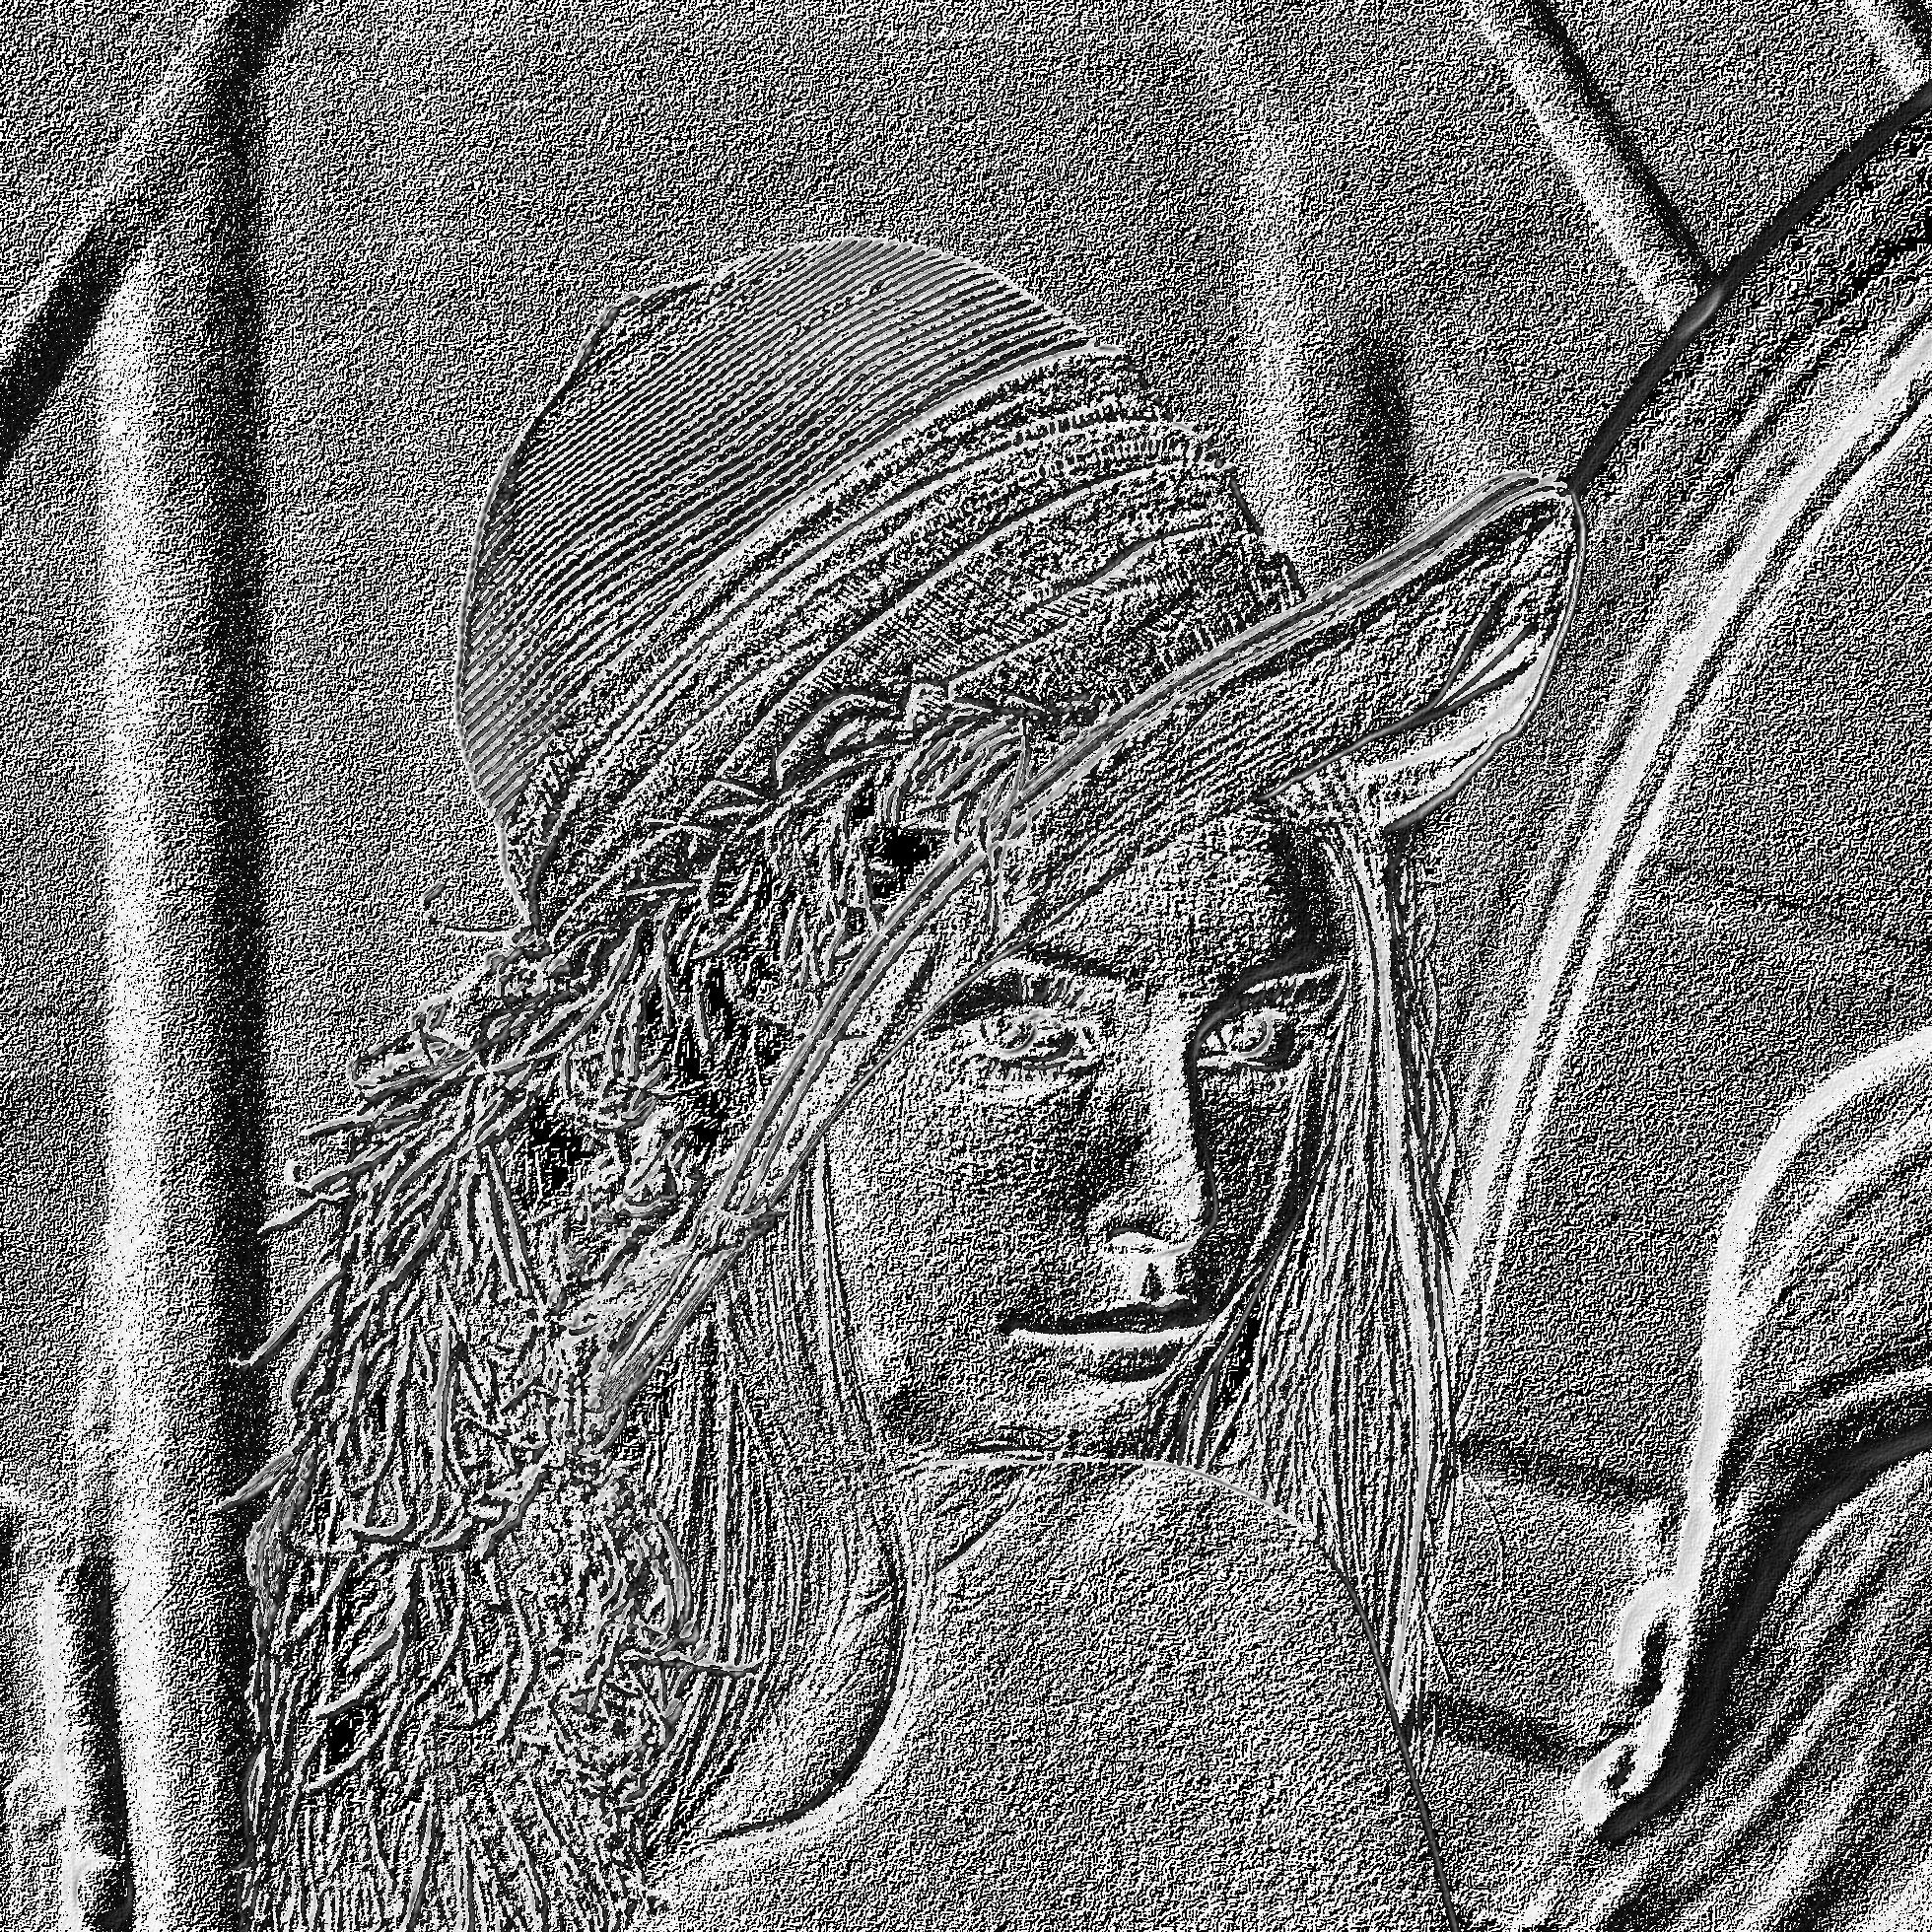
\includegraphics[width=7cm]{resources/modified/lena/lena_emboss_1.jpg}
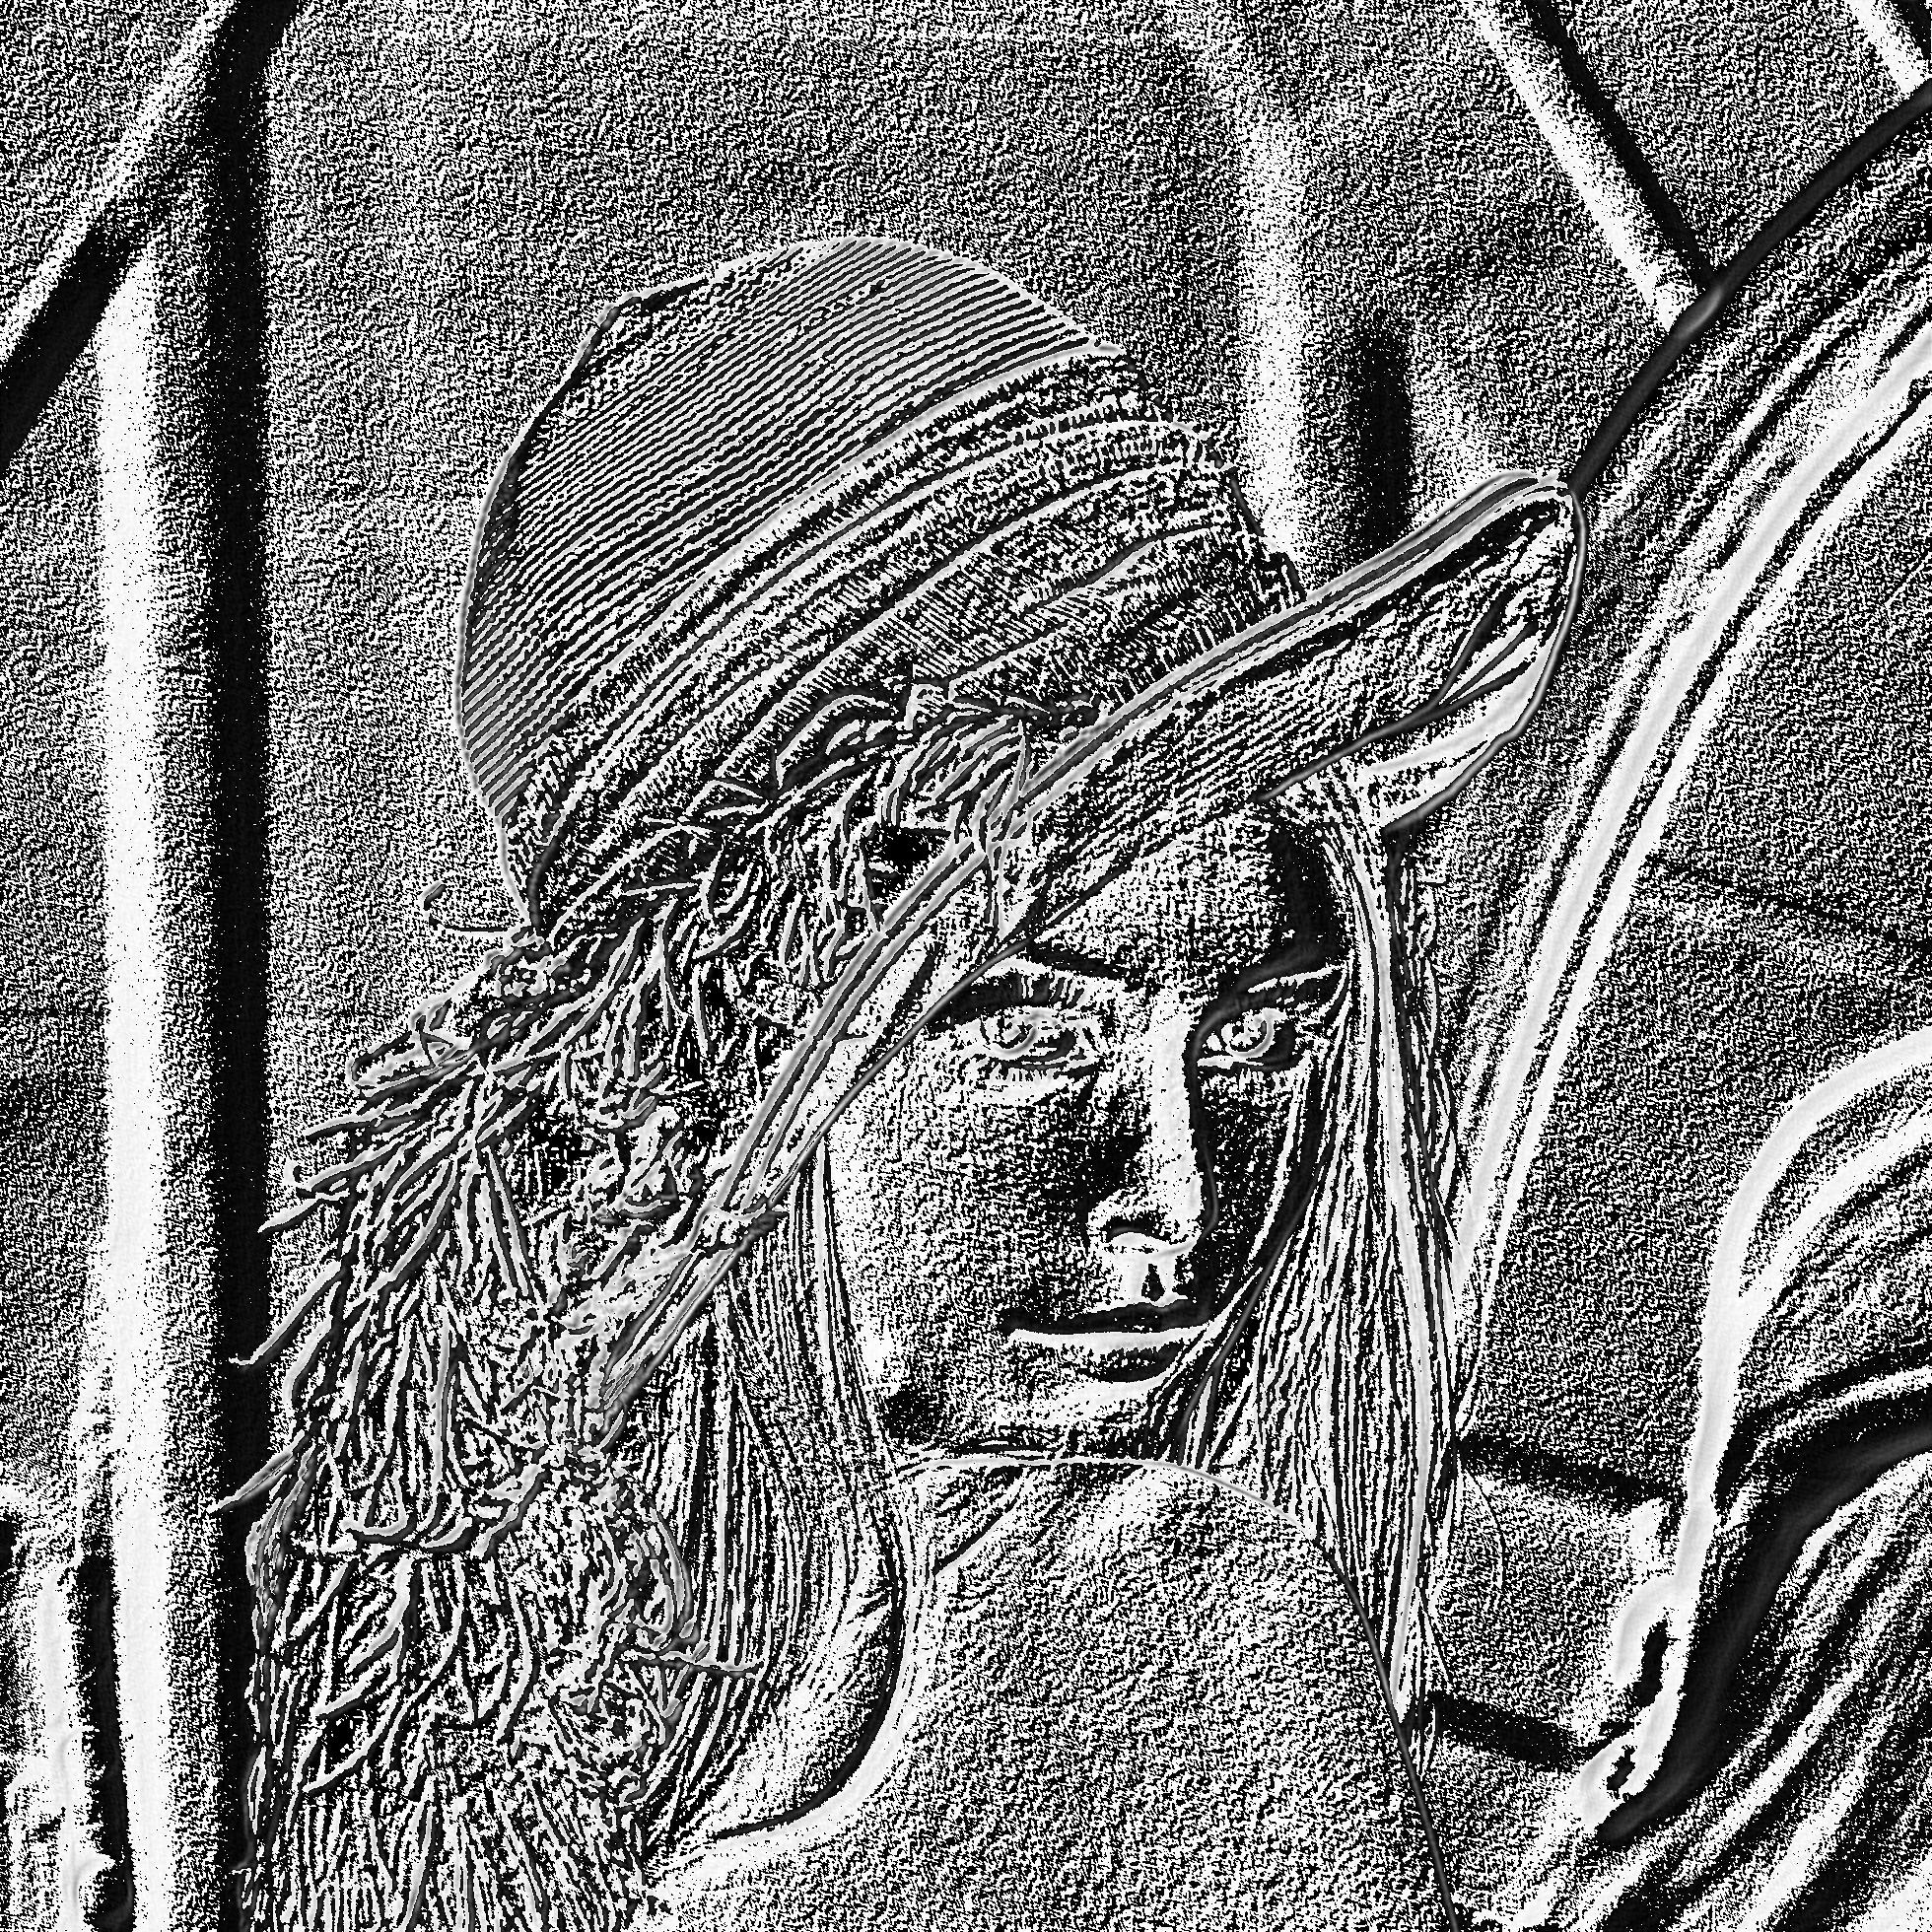
\includegraphics[width=7cm]{resources/modified/lena/lena_emboss_2.jpg}
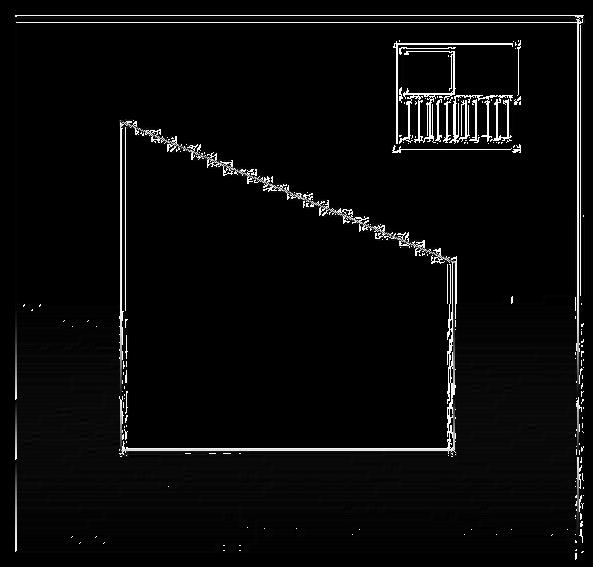
\includegraphics[width=7cm]{resources/modified/sample/sample_emboss_1.jpg}
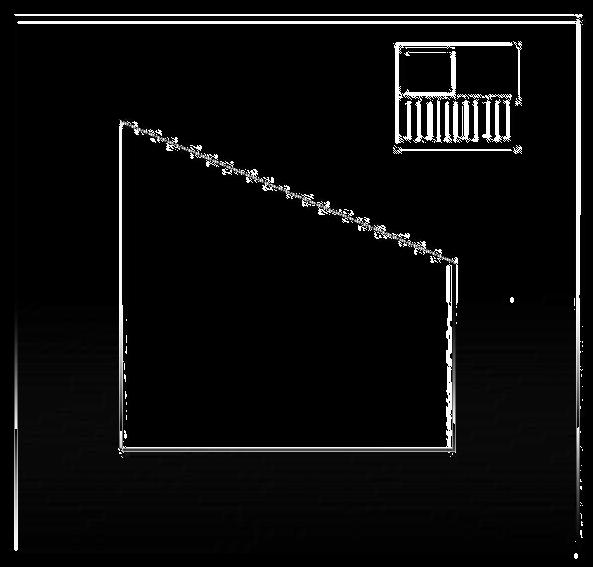
\includegraphics[width=7cm]{resources/modified/sample/sample_emboss_2.jpg}\\
\pagebreak
\text{wyniki działania filtrów typu "ridge detection":}\\
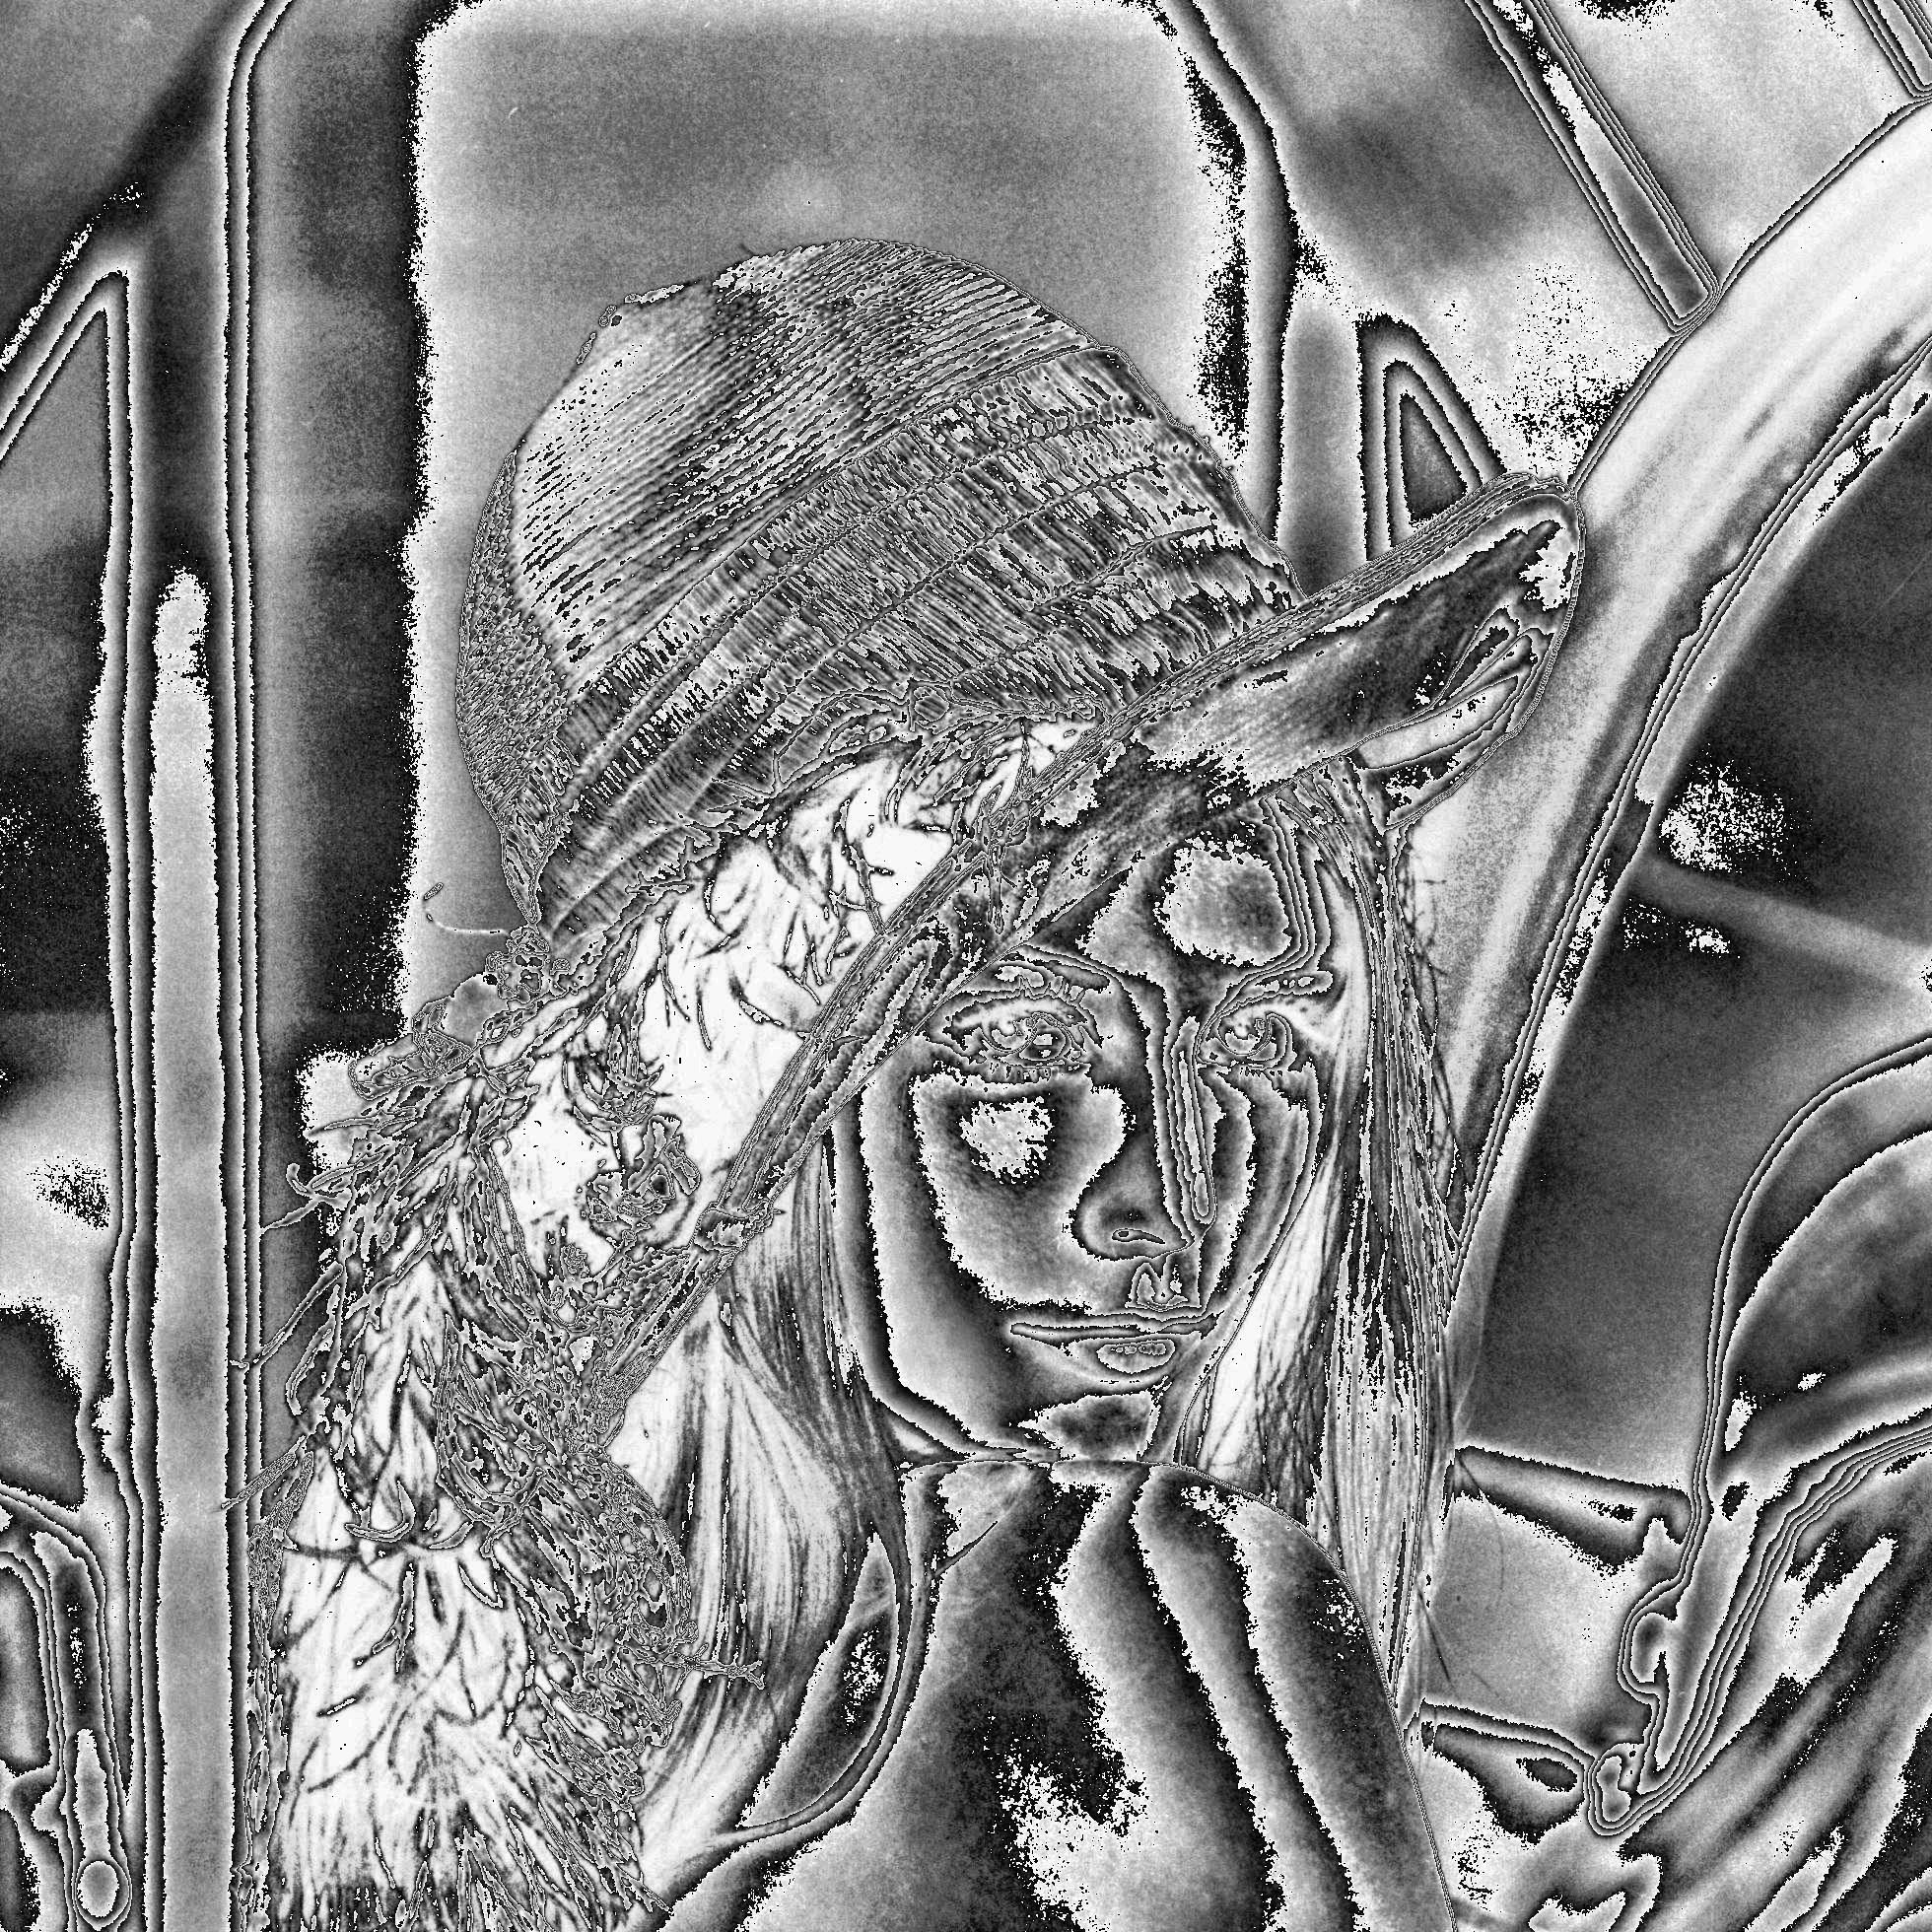
\includegraphics[width=7cm]{resources/modified/lena/lena_ridge_detection_1.jpg}
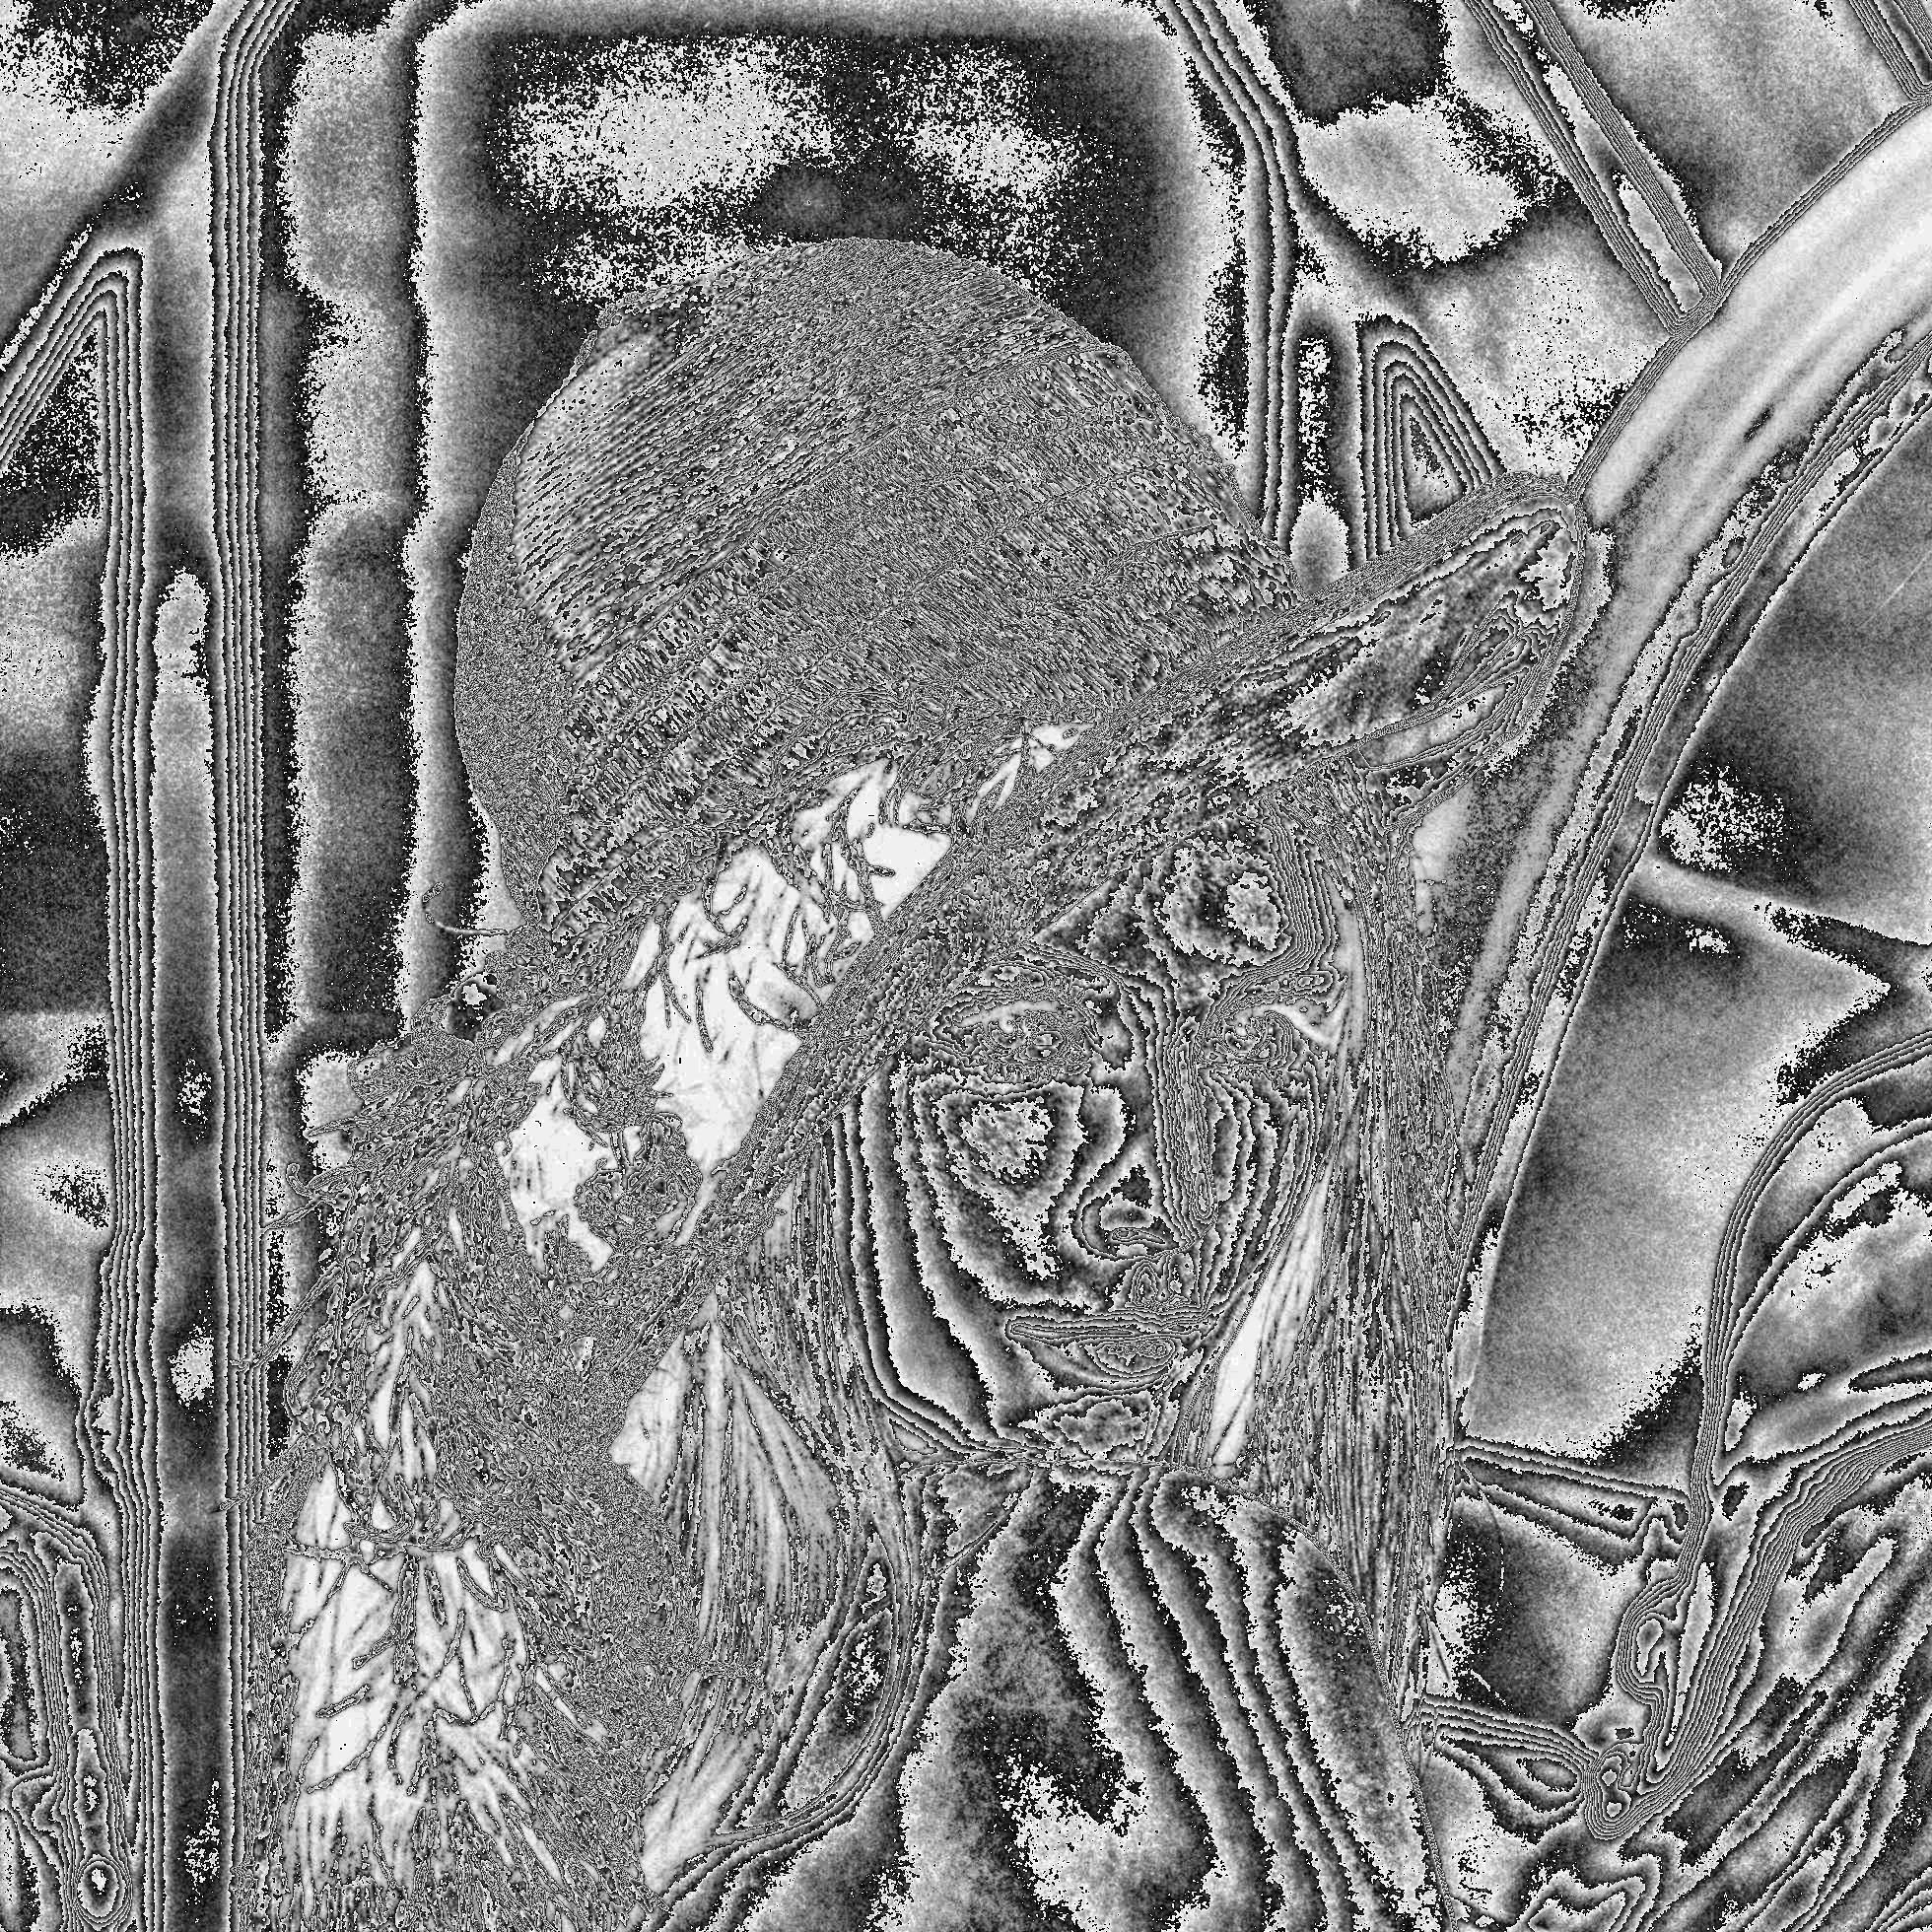
\includegraphics[width=7cm]{resources/modified/lena/lena_ridge_detection_2.jpg}
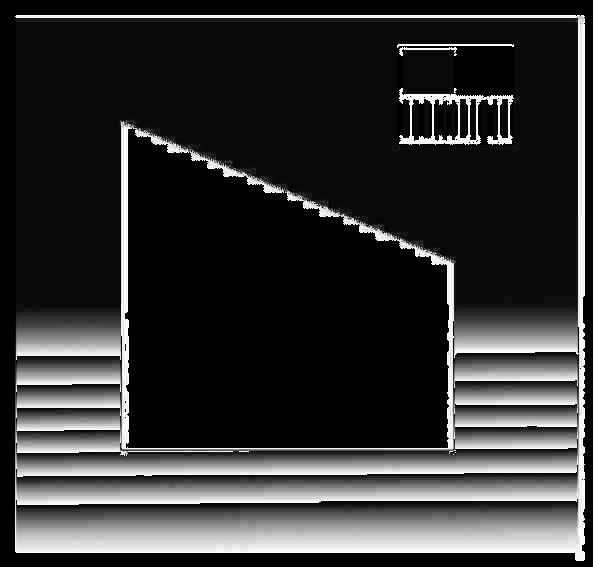
\includegraphics[width=7cm]{resources/modified/sample/sample_ridge_detection_1.jpg}
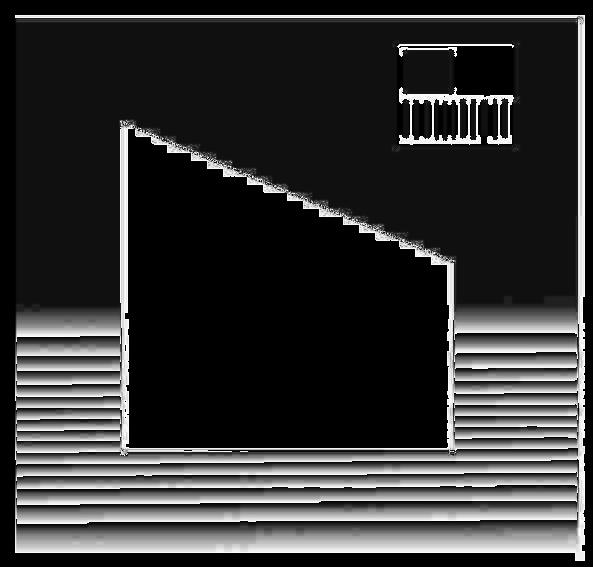
\includegraphics[width=7cm]{resources/modified/sample/sample_ridge_detection_2.jpg}
\end{center}

%%%%%%%%%%%%%%%%%%%%%%%%%%%%%%%%%%%%%%%%%%%%%%%%%%%%%%%%%%%%%%%%%%%%%%%%%%%%%%%%%%%%%%%%%%%%%%%%%%%%%%%%%%%%%%%%%%%%
%%%%%%%%%%%%%%%%%%%%%%%%%%%%%%%%%%%%%%%%%%%%%%%%%%%%%%%%%%%%%%%%%%%%%%%%%%%%%%%%%%%%%%%%%%%%%%%%%%%%%%%%%%%%%%%%%%%%
\chapter{Wnioski}

\paragraph{\indent Wykorzystując odpowiednie filtry należy pamiętać o tym jak zależą jego efekty w stosunku do jego wielkości. Filtr wykorzystany nieoptymalnie może dać odwrotne efekty od oczekiwanych. W celu lepszego poznania charakterystyki filtru można wykonać kilka testów na rożnych obrazach w różnych wariacjach filtru.}


%%%%%%%%%%%%%%%%%%%%%%%%%%%%%%%%%%%%%%%%%%%%%%%%%%%%%%%%%%%%%%%%%%%%%%%%%%%%%%%%%%%%%%%%%%%%%%%%%%%%%%%%%%%%%%%%%%%%%%%%%%%
\chapter{Dodatkowe}
\paragraph{Do wykonania zamieszczonych obrazów wykorzystałem napisane przeze mnie skrypty w Pythonie i Matlabie. Wszystkie skrypty oraz dodatkowe przefiltrowane obrazy są zamieszczone w \href{https://github.com/FilipM13/CPS}{moim repozytorium na githubie}.}

\end{document}